% !TeX spellcheck = en_US
% !TeX encoding = UTF-8

% COMPILE WITH:
% `latexmk`
% You need lualatex and biber (in all TeXLive distributions)

\documentclass[
    numbers=noenddot,
    %listof=totoc,
    parskip=half-,
    fontsize=12pt,
    paper=a4,
    oneside,
    titlepage,
    bibliography=totoc,
    chapterprefix=false,
%    draft
]{scrbook}

% use lualatex or xelatex
%\usepackage{fontspec}
\usepackage{graphicx}
\usepackage[onehalfspacing]{setspace}

% better language support
%\usepackage{polyglossia}
%\setdefaultlanguage{english}
%\setotherlanguage{german}

\usepackage{tocbasic}
\usepackage{booktabs}
\usepackage{multicol}
\usepackage{multirow}

\usepackage[]{scrlayer-scrpage}

% better bibliography (biblatex style)
% use biber to compile
\usepackage[citestyle=alphabetic, bibstyle=alphabetic, sorting=nyt, backend=biber, language=english, backref=true, maxcitenames=2]{biblatex}

% better quotes
% use \enquote{text}
\usepackage[autostyle,english=american,german=quotes]{csquotes}
\addbibresource{bibliography.bib}

% appendix
\usepackage[titletoc]{appendix}

% where to put all images and figures
\graphicspath{{images/}}

% YOUR PACKAGES
\usepackage{placeins}
\usepackage[utf8]{inputenc}
\usepackage{tabularx}
\usepackage{fancyvrb}
\usepackage{listings}
\usepackage{adjustbox}
\usepackage[table,xcdraw]{xcolor}
\usepackage{lipsum}
\usepackage{minted}
\usepackage{pdfpages}
\usepackage[acronym]{glossaries}
\usepackage[automake]{glossaries-extra}
\makeglossaries
\newglossaryentry{latex}
{
    name=latex,
    description={Is a markup language specially suited 
    for scientific documents}
}

\newglossaryentry{maths}
{
    name=mathematics,
    description={Mathematics is what mathematicians do}
}


\newacronym{dfg}{DFG}{Deutsche Forschungsgemeinschaft - A funding organization that supports academic research and scientific collaboration in Germany}
\newacronym{pdf}{PDF}{Portable Document Format - A file format that is used to present and exchange documents in a manner independent of software, hardware, and operating systems}
\newacronym{png}{PNG}{Portable Network Graphics - A file format that is used for storing raster graphics (bitmap images) with lossless compression}
\newacronym{jpg}{JPEG/JPG}{Joint Photographic Experts Group - the name of the organization that developed the JPEG image compression standard. JPEG files are a file format for storing and transmitting digital images}
\newacronym{api}{API}{Application Programming Interface - A set of rules and protocols that enables different software applications to communicate with each other by providing a standardized interface}
\newacronym{ui}{UI}{User Interface - All visual and interactive elements of a software application that an user interacts with}
\newacronym{ocr}{OCR}{Optical Character Recognition - An OCR system converts printed or handwritten text into machine-encoded text}
 


% Title
\title{Metadata Extraction in Scientific Publications}

% Author
\author{Bastian Birkeneder}

% Date
\date{\today}

% CHOOSE ACCORDINGLY
%\newcommand{\thesisType}{Bachelorarbeit}
\newcommand{\thesisType}{Masterarbeit}

\makeatletter
\let\thetitle\@title
\let\theauthor\@author
\let\thedate\@date
\makeatother

\pagestyle{scrheadings}

\begin{document}

%%%%%%%%%%%%%%%%%%%%%%%%%%%%%%%%%%%%%%%%%%%%%%%%%%%%%%%%%%%%%%%%%%%%%%%%%%%%%%%%%%%%%%%%%
\frontmatter
% CHOOSE ACCORDINGLY
%% !TeX spellcheck = en_US
% !TeX encoding = UTF-8
\begin{titlepage}
    \centering
    \begin{onehalfspace}
    
        	
\includegraphics[width=7cm]{uni-logo.png}\\
        	\vspace{1.0cm}
        	\large {\bfseries Lehrstuhl für Data Science \\

        	\vspace{2.5cm}

            \begin{doublespace}
            	{\textsf{\Huge{\thetitle}}}
            \end{doublespace}

        	\vspace{2cm}

            \Large{Bachelorarbeit von}\\

        	\vspace{1cm}

        	{\bfseries \large{\theauthor}}

        	\vfill

        	{\large
        		\begin{tabular}[l]{cc}
        			\textsc{Prüfer}\\
        			Prof.~Dr.~Michael Granitzer
        		\end{tabular}
        	}

        	\vspace{1.5cm}

        	\parbox{\linewidth}{\hrule\strut}

            \vfill

	    {\thedate}
    	
    \end{onehalfspace}
\end{titlepage}

% !TeX spellcheck = en_US
% !TeX encoding = UTF-8
\begin{titlepage}
    \centering
    \begin{onehalfspace}
    	
        	
\includegraphics[width=7cm]{uni-logo.png}\\
        	\vspace{1.0cm}
        	\large {\bfseries Lehrstuhl f\"ur Data Science }\\

        	\vspace{2.5cm}

            \begin{doublespace}
            	{\textsf{\Huge{\thetitle}}}
            \end{doublespace}

        	\vspace{2cm}

            \Large{Masterarbeit von}\\

        	\vspace{1cm}

        	{\bfseries \large{\theauthor}}

        	\vfill

        	{\large
        		\begin{tabular}[l]{cc}
        			\textsc{1.~Pr\"ufer} & \textsc{2.~Pr\"ufer} \\
        			Prof.~Dr.~Michael Granitzer& Prof.~Dr.~Harald Kosch
        		\end{tabular}
        	}

        	\vspace{1.5cm}

        	\parbox{\linewidth}{\hrule\strut}

            \vfill

	    \thedate
    \end{onehalfspace}
\end{titlepage}


%\setcounter{tocdepth}{3}
\tableofcontents
\newpage

% -- ABSTRACT
% !TeX spellcheck = en_US
% !TeX encoding = UTF-8
\chapter*{Abstract}
Metadata, or data about data, refers to information that provides structured context and details about other data. In the context of scientific publications, metadata can facilitate the discovery process of those publications and help researchers in exploring the enormous landscape of scientific literature.\\
In this thesis, we delve into the exploration of techniques for the extraction and parsing of essential metadata, such as article authors and references, from scientific publications. We propose our novel and effective approach to extract metadata both from the article itself and from the references within the publication.\\
Our tool, BiBEx, is designed to accurately extract metadata from both historical and contemporary scholarly literature, encompassing texts in both English and German. To accomplish this, we curated two distinct datasets: one dedicated to document segmentation and the other focused on reference segmentation and parsing.\\
Our results demonstrate that BiBEx achieves comparable or slightly improved performance when compared to commonly used tools for metadata extraction in scientific literature.
\newpage

% -- Acknowledgements (optional)
% !TeX spellcheck = en_US
% !TeX encoding = UTF-8
\chapter*{Acknowledgments}
I would like to express my sincere gratitude to all those who have contributed to the completion of this thesis. This work would not have been possible without the support, guidance, and encouragement of numerous individuals and organizations.\\
First and foremost, I would like to extend my heartfelt appreciation to my late employer, Prof. Dr. Malte Steinbrink. The passing of Malte Steinbrink has left an irreplaceable void in our academic community and at the Chair of Human Geography. I am forever grateful for his unwavering support, patience, mentorship, and profound expertise.\\
I am grateful to my advisor, Dr. Philipp Mayr-Schlegel, for his valuable guidance, feedback, and scholarly expertise throughout the thesis process.\\
I am indebted to my colleagues and fellow researchers, whose support and collaboration have been invaluable throughout this journey. I want to thank all members of the Chair of Human Geography, who generously contributed their time and expertise in the annotation process.\\
Although the completion of this thesis is accompanied by a sense of sadness, as we remember the profound loss of Malte Steinbrink, I am grateful for the time we shared together. His dedication and passion for our research project have left a lasting impact on this work, and I would like to honor his memory in this endeavor.
\newpage

% -- List of figures
\thispagestyle{empty}
\cleardoublepage
\listoffigures
\newpage

% -- List of tables
\thispagestyle{empty}
\cleardoublepage
\listoftables
\newpage

%%%%%%%%%%%%%%%%%%%%%%%%%%%%%%%%%%%%%%%%%%%%%%%%%%%%%%%%%%%%%%%%%%%%%%%%%%%%%%%%%%%%%%%%%
\mainmatter

% -- Chapters
% following IMRaD structure
% adjust for your liking
\chapter{Introduction}\label{chap:introduction}
In this thesis, we propose a methodology of cascading sequence labeling models to extract metadata from scientific publications. The following chapter offers a compact introduction to the problem domain (Section \ref{sec:problem_domain}), provides a short overview over the GEOcite project (Section~\ref{sec:geocite}), presents the problems encountered in the GEOcite metadata extraction process and questions we are trying to answer (Section~\ref{sec:research_questions}), and provides an outline for the rest of this thesis (Section~\ref{sec:structure}). 

\section{Metadata in Scientific Publications}\label{sec:problem_domain}
Metadata, or literally \enquote{data about data}, as a concept, has existed since ancient times and in our increasingly digital world, we continue to interact with metadata more frequently than ever before.\\
Historically, the primary focus of library metadata has been to enable access to analog collections. As such, library metadata encompasses indexes, abstracts, and bibliographic records that adhere to cataloging standards such as the Anglo-American Cataloguing Rules (AACR) and the Machine-Readable Cataloging (MARC) format.\\
Online databases, such as bibliographic utilities, online public access catalogs (OPACs), and for-profit databases like Scopus, made the results accessible to a wide range of users~\cite{schmidt1997libraries}.\\
Constant technological advancements in automated data processing, like metadata mining and web crawling, as well as a increasing number of elaborate standards and concepts like the Resource Description Framework (RDF) and the Semantic Web, suggest the automation of metadata procession is expected to increase further~\cite{gill2008introduction}.
\newpage

An ever-growing amount of academic publications and journals per year~\cite{fire2019over} can impede effective data discovery for researchers. Metadata of scholarly work, consisting of information about the title, authors, abstracts, research topics, and keywords, plays a vital role in indexing for search engines like Scopus or Google Scholar~\cite{ahmar2018lecturers}. This facilitates the effective exploration and discovery of scientific publications, enabling scientists to locate and access relevant work within their fields of interest. By leveraging comprehensive metadata, researchers can navigate the vast landscape of scholarly literature with greater efficiency and precision by filtering unrelated information in their search queries.\\
Furthermore, Metadata can help with long term tracking and preservation of scholarly work. While storing and conserving whole publications is only possible with specific open licenses, metadata of those aforementioned articles generally do not fall under copyright protection~\cite{cox2017metadata}. This allows the creations of large digital archives to permanently store data for tracking, preservation, and an open or commercial exchange, independent of the copyright holder.\\
Metadata also helps with tracking of citations in scientific work by establishing links between citing and cited publications, creating graph-like networks. Online databases like Crossref~\cite{bartell_crossref_nodate} and DataCite~\cite{noauthor_datacite_nodate} enable citation linking independent of an article's publisher. Author-level metrics like the h-index~\cite{hirsch2005index} quantify the impact of a researcher's work and provide a theoretical evaluation of his/her academic career.\\
In the context of this thesis, we are foremost interested in two categories of metadata in scientific publications
\begin{itemize}
    \item metadata about the publication itself. Information, which can by itself or combined identify a document, for example, authors, title, abstract, or the date. Since it resides often in the header section of an essay, we will simply refer to it as \enquote{header metadata}.
    \item metadata about the cited scholarly work within a publication. Using the same aforementioned principle, we will refer to it as \enquote{reference metadata}.
\end{itemize}
Naturally, the question arises of how we can actually gather this data automatically, given an arbitrary scholarly article.
An intuitive first approach could resolve around unique identifiers of a documents. Persistent identifier, such as the Digital Object Identifier (DOI), International Standard Serial/Book Number (ISSN/ISBN), or the Publisher Item Identifier (PII) can be extracted from a document using simple regular expressions.
\newpage

The regular expression
\begin{Verbatim}[fontsize=\small]
/^10.\d{4,9}/[-._;()/:A-Z0-9]+$/i
\end{Verbatim}
matches 99.3\% of all of Crossref's DOIs~\cite{Gilmartin_2015}. The resulting identifier can then be used to query metadata about the publication directly from the Crossref or DataCite API.\\
This trivial approach falls short in reality, as we can not always reliably extract an unique identifier. The DOI standard, for example, was established in the year 2000. A theoretical algorithm utilizing DOIs for metadata queries would not be able to gather data about a publication written before the year 2000.\\
Furthermore, we might extract multiple identifiers, since DOIs can also be attributed to referenced literature.

\section{GEOcite}\label{sec:geocite}
To fully understand the underlying problem, we want to briefly introduce the GEOcite project, which essentially deals with the question of how we can automatically extract metadata from a large corpus of scholarly work. We further want to show shortcomings of this approach and illustrate, how recent advancements in Machine Learning (ML) might help to bridge this gap.

\subsection*{The GEOcite Project}
GEOcite is a research project funded by the German Research Council (DFG), which aims to make an empirical contribution to the scientific discussion about the practice of interdisciplinary work using the example of geography by means of network-analytical and bibliometric analysis \cite{geocite}.\\
It is designed as the direct continuation of the DFG project \enquote{Die Säulen der Einheit und die Brücken im Fach}\cite{geocite_dfg}, which aims to identify and analyze the interdisciplinary structures within the German-speaking scientific community in the field of Geography. While the previous research work was limited on presently existing structures, the focus of the current phase lies on the temporal evolution of this research network.\\
To investigate these relations within the Geography research community, the GEOcite project intends to analyze the citation behaviour of all German-speaking post-war professors in the DACH region since 1949. Resulting insights may contribute towards exploration of the genesis of various subdisciplines within the field of Geography, or examine the temporal shifting role of female researchers in this specific academic circle.
Subsequently, the resulting, graph-like citation networks can be evaluated using network analytical methods \cite{aufenvenne2014saulen}.\\
As a first step to create a citation network, a comprehensive database of all Geography professors from Germany, Austria, and Switzerland, which were active between 1949 and the present day was created \cite{geoprof}. Within the context of this thesis, members of this collated group of professors are also referred as actors.\\
In the following sections, we will briefly describe the fundamental architecture of GEOcite and current data transformation processes as well as drawbacks and possible improvements, suggested in this thesis.

\begin{figure}
	\centering
	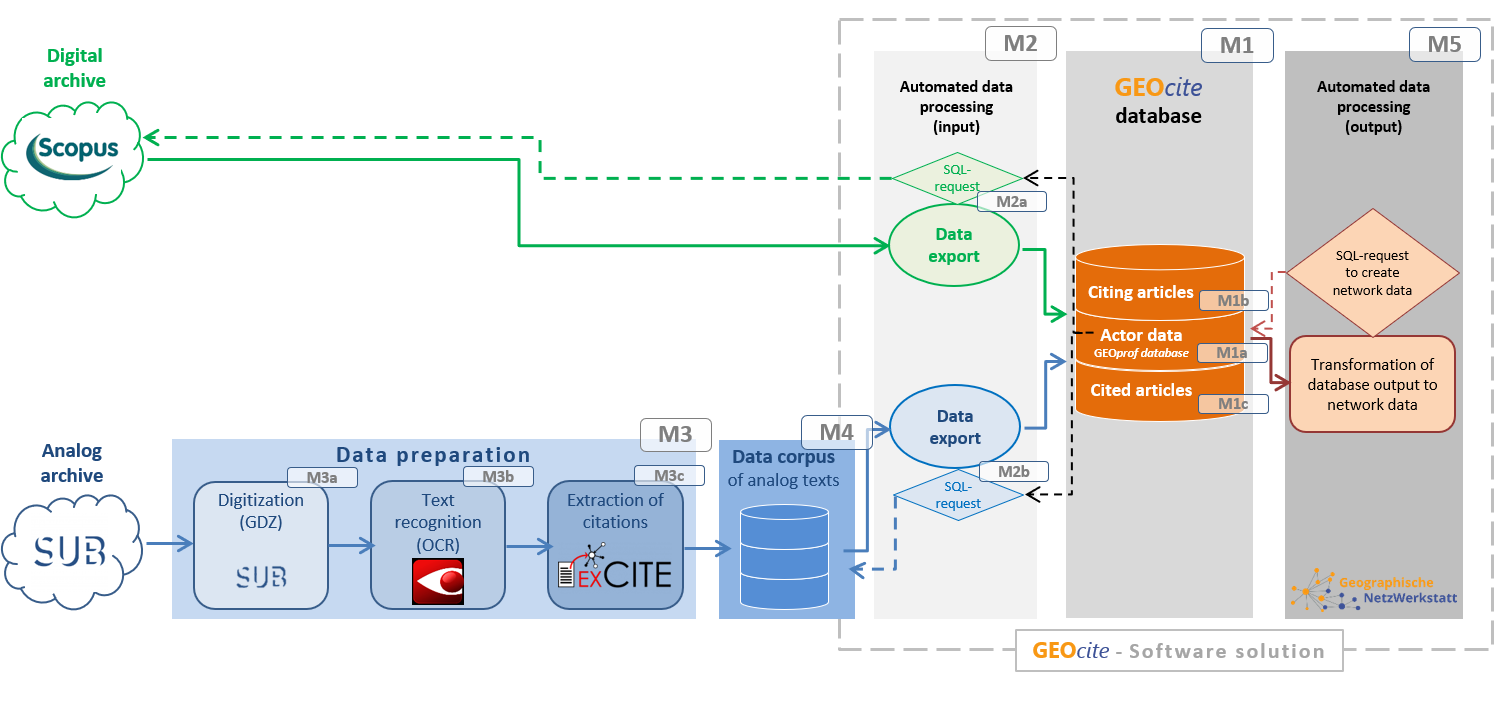
\includegraphics[width=1.0\linewidth]{images/geocite_dataflow_eng.png}
	\caption{The conceptional workflow of GEOcite.}
	\label{fig:geociteConcept}
\end{figure}

\subsection{Literature Sources}
The relevant literature is extracted from two distinguished data sources: from the citation database Scopus, in context of GEOcite referred as \enquote{digital archive}, as well as from a collection of analog scans of various journals, also referred as \enquote{analog archive}.\\
While Scopus is mainly used to gather metadata from recent publications of relevant actors and already provides parseable citation data via an API, the analog literature collection contains mostly articles from earlier years and requires several data processing steps to extract relevant information. Our analog corpus consists of 20,190 documents, predominately (85\%) in German. A large minority (14\%) consists of publications written in English. The remaining documents (1\%) are mainly of French and Spanish origin. In the scope of this thesis, we are primarily interested in the extraction process of citation data from the analog archive.

\subsubsection{Data Processing of Analog Data}
After the identification of relevant journals, articles are scanned and undergo several automatic pre-processing steps like conversion to grey scale images, skew correction, and noise removal. An OCR software is then applied to the processed scans, which are subsequently converted to PDF files with the corresponding text layer.\\
In the next processing step useful metadata about the article itself is extracted, for example author names, article title, journal, DOI, and date, which is needed to match an author of an article with an identified actor.\\
To extract this necessary header information about an scientific essay, the open-source software GROBID \cite{lopez2009grobid} is used. While it also possible to extract citation data with GROBID, GEOcite utilizes the EXCITE toolchain for this step~\cite{excite_toolchain}, specifically the EXParser component. Both EXParser and GROBID use a cascading composition of Machine Learning (ML) models to extract citation data. EXParser, however is specifically trained on German scholarly literature and is therefore more suited to our analog corpus. We will take a more detailed look on EXParser and GROBID in Chapter~\ref{chap:related}.

\section{Research Questions}\label{sec:research_questions}
The employment of two complementary tools to extract relevant information may cause friction under certain circumstances. Changes in IT infrastructure or updates can cause unforeseen compatibility issues. Modifications of existing processing routines can generate overhead work and prolong maintenance work. An unified tool, capable obtaining both header information, as well as citation data is therefore preferable.\\
Of all documents in our corpus, which are written in English, 91\% were published after the year 2000. This suggests that the trend to publish increasingly scholarly literature in English \cite{di2017publish} can also be observed in our corpus. GEOcite is designed as continuous project, with an ever expanding online and analog literature collection. Since EXParser is trained on scientific essays written mostly in German, we expect a declining performance on newly published literature, simultaneously historical documents become more accessible. To allow a future-proof data mining process, we require a ML model capable of extracting metadata from publications written either in German or English.\\
The processing pipeline of GEOcite involves the crucial step of transforming analog text into digital representations. To achieve this, OCR is employed to convert the physical documents into a machine-readable format. However, it is important to acknowledge that the OCR process is not infallible and can introduce errors or inaccuracies. Therefore, the aim is to construct a robust system that can effectively handle these imperfections.\\
Both GROBID and EXParser utilize Conditional Random Fields (CRF) as backbone for their information retrieval process, relying on textual and layout features. Visual information has proven to be valuable and effective when extracting data from visual-rich documents~\cite{cui2021document}. Continuous advances in Deep Learning, especially in the fields of Computer Vision, Natural Language Processing (NLP) and DocumentAI, suggest that these technologies can be used to improve the results of our extraction process.\\
We want to address these issues in this thesis, and want to offer a unified and robust solution for the metadata extraction process, utilizing state-of-the-art ML technologies and capable of working on multilingual literature. To explicitly summarize the aforementioned ideas, we want to answer the questions, if we can
\begin{itemize}
    \item simplify the structure of the extraction process and condense the functionally in one tool?
    \item employ a mostly language independent extraction process by utilizing multilingual ML models?
    \item create a robust system, that is able to handle impurities in our data?
    \item improve our overall extraction process by utilizing state-of-the-art ML technologies and techniques?
    \item include visual information to improve the results of our extraction process?
\end{itemize}

\section{Structure of the Thesis}\label{sec:structure}
In Chapter~\ref{chap:background}, we provide the background material for this thesis. Chapter~\ref{chap:related}, contains related approaches, available software solutions, and datasets related to our problem domain. Chapter~\ref{chap:methods} explains the methods, we used to answer our research questions. We provide a conceptual framework, explain our approach, and describe our data collection as well as the models employed. In Chapter~\ref{chap:bibex} we present our application, BiBEx, we developed to address the problems encountered in the GEOcite metadata extraction approach. The results of our overall system evaluation as well as the component evaluation of our system are presented in Chapter~\ref{chap:results}. We discuss our results and the limitations of our work in Chapter~\ref{chap:discussion} and conclude our thesis in Chapter~\ref{chap:conclusion} and highlighting potential future work.

\chapter{Background}\label{chap:background}
In solving sequence-to-sequence problems, such as machine translation (MT), where a ML algorithm translates speech or text to different languages, Recurrent Neural Networks (RNN) have been widely utilized in an encoder-decoder architecture, surpassing many other ML algorithms in performance~\cite{cho2014properties}. The encoder network takes the input data and generates a compact vector representation, which is then used as input for the decoder network. The decoder network unrolls over time to generate the output sequence based on the input and its internal state.\\
However, RNN face challenges with long sequences due to the vanishing gradient problem, which results in the model losing meaningful information about token at the start of a sequence~\cite{hochreiter1998vanishing}. To address this issue, improvements in architecture have been introduced, such as Long Short-Term Memory (LSTM)~\cite{hochreiter1997long} and Gated Recurrent Unit (GRU)~\cite{cho2014learning} models, which aim to preserve information from the entire sequence.\par
In recent years, the Transformer architecture, introduced by Vaswani et al.~\cite{vaswani2017attention}, has gained prominence. Similar to the RNN encoder-decoder architecture, it consists of an encoding and decoding component. The encoding component is a stack of encoder layers, and the decoding component is also a stack of decoder layers, both equal in number.\\
Each layer in the Transformer architecture consists of two sub-layers: a self-attention layer and a feed-forward neural network. The key difference between RNN and the Transformer lies in the self-attention sub-layer. This unique component enables the Transformer to consider all hidden states from the encoder sequence when making predictions. In the RNN encoder-decoder architecture the decoder is presented only with the final output of the encoder layer. The attention based architecture, on the other hand, allows a model to attend every hidden state from each encoder node at every time step, which allows Transformer models to effectively handle long sequences.\par
\textit{BERT} (\textbf{B}idirectional \textbf{E}ncoder \textbf{R}epresentations from \textbf{T}ransformers), introduced by Devlin et al.~\cite{devlin2019bert}, is a language model designed to learn general language representations. At its core, it is a multi-layer bidirectional Transformer encoder stack that is pre-trained on a large corpus.\\
BERT uses WordPiece embeddings~\cite{wu2016google} with a vocabulary size of 30,000 tokens. Unknown words not represented in the vocabulary are embedded as a special unknown token ($[UNK]$). The first token in each input sequence is denoted as a special classification token ($[CLS]$). Sentence pairs are processed as one input sequence separated by a special character ($[SEP]$), and a learned embedding is assigned to each token to represent the sentence it belongs to.\\
The final input embedding consists of the summarized token embeddings, segment embeddings, and position embeddings of each token in the sequence. The authors present two architecture configurations that differ in the number of Transformer blocks, hidden size, and number of self-attention heads.
For the pre-training phase, they propose two unsupervised objectives:\\
The first is Masked Language Modeling (MLM), where a portion of the token in the input sequence are masked and replaced with a special mask token ($[MASK]$). During the pre-training the model predicts the masked token to learn a deep bidirectional representation. To avoid a mismatch between the training and fine-tuning process, token chosen to be masked are only masked 80\% of the time. In 10\% of the time, token are replaced by a random token and in the remaining 10\%, token are left as they are.\\
The second is Next Sentence Prediction (NSP), which allows the model to learn sentence relationships. Two sentences, A and B, are chosen from the training corpus and the model has to predict if sentence B follows sentence A. In 50\% of theses cases, sentence B succeeds sentence A. In the remaining cases sentence B is chosen randomly from the corpus.\\
The self-attention mechanism allows fine-tuning BERT for various different NLP tasks, which resulted in many broken records for language-based tasks~\cite{sun2019fine,nogueira2019passage,zampieri2019semeval}.\par
Liu et al. introduced \textit{RoBERTa} (\textbf{R}obustly \textbf{o}ptimized \textbf{BERT} \textbf{a}pproach)~\cite{liu2019roberta}, which presents an optimized version of BERT with a series of improvements. Instead of using fixed masking patterns for sequences, they propose dynamic masking, where the masking pattern is generated each time a sequence is fed to the model. They also remove the Next Sentence Prediction (NSP) objective and utilize full sentences sampled contiguously from one or more documents. In addition, they employ larger mini-batches to improve optimization speed and end-task performance. Lastly, RoBERTa utilizes a larger vocabulary with Byte-Pair Encoding (BPE)~\cite{sennrich2016neural}, which is a hybrid approach combining character- and word-level representations of token. This embedding relies on subword token, gathered through statistical analysis of the training corpus.\par
Conneau et al. introduced \textit{XLM} (Cross-Lingual \textbf{L}anguage \textbf{M}odel)~\cite{conneau2019cross} with the goal of extending the pre-training approach to multiple languages to enable cross-lingual understanding (XLU). They adopted the BPE algorithm to generate a shared vocabulary of subwords for all languages. For pre-training XLM, they employed several objectives.\\
One of them is Causal Language Modeling (CLM), where the objective is to predict the next word given the previous words in a monolingual sentence.\\
They also utilized the MLM objective on monolingual input sentences, similar to BERT, where random tokens are masked for the model to predict. Instead of using sentence pairs as in BERT, they used text snippets with a random number of sentences. Additionally, the authors used weights to balance the disproportional frequencies of tokens.\\
The Translation Language Modeling (TLM) objective is a supervised task where parallel sentences in different languages are masked. The model must predict the masked token by attending to the surrounding words in the same language or in the translation sentence.\\
Similar to BERT, the input embedding for XLM includes token embeddings, position embeddings, and language embeddings.\\
At the time of its introduction, XLM outperformed several state-of-the-art models in machine translation benchmarks.\par
\textit{XLM-RoBERTa} (XLM-R) is a Transformer-based multilingual masked language model introduced by Conneau et al.~\cite{conneau2019unsupervised}, which draws inspiration from the XLM approach. The authors formulate the \enquote{curse of multilinguality}, which refers to a tradeoff point where including more languages can improve cross-lingual performance for low-resource languages. However, beyond that threshold, the overall performance on both monolingual and cross-lingual benchmarks starts to worsen.\\
XLM-R utilizes a Transformer encoder model, trained solely with the MLM objective, similar to the XLM approach. For tokenization, they use subwords, but instead of BPE, they employ SentencePiece~\cite{kudo2018sentencepiece} with a unigram language model~\cite{kudo2018subword} and a large vocabulary of 250k subwords. The authors also remove the language embeddings from the input embeddings, which were introduced in XLM, to facilitate improved code-switching.\\
XLM-R is trained on 100 languages using a large CommonCrawl Corpus with a size of 2.5 TB. The authors provide two model configurations to enable comparisons with BERT. In their evaluation, they compare their results against XLM and mBERT, a BERT Transformer pre-trained on a multilingual corpus. XLM-RoBERTa achieves state-of-the-art performance on multiple cross-lingual tasks, including cross-lingual classification, sequence labeling, and question answering.\par
\textit{LayoutLM}, proposed by Xu et al.~\cite{xu2020layoutlm}, is a novel Transformer model designed to incorporate text, layout, and visual information from documents. The authors aim to leverage two additional features alongside the input text: Document Layout Information, which captures the relative position of each token in the document, and Visual Information, which captures essential features in Visual Rich Documents (VRD).\\
To integrate both features, the authors introduce two modifications to the BERT architecture: a 2-D position embedding and an image embedding.\\
The 2-D position embedding encodes the relative position of a token as a bounding box $(x_0, y_0, x_1, y_1)$, where $(x_0, y_0)$ is the location of the upper left corner, and $(x_1, y_1)$ represents the position of the lower right corner. Each coordinate dimension shares the same embedding table, resulting in four position embedding layers, each corresponding to one coordinate in the bounding box.\\
For the image embedding, the document images are divided into pieces based on the bounding boxes of each token. Image region features are then generated using a Faster R-CNN model~\cite{girshick2015fast} for these image parts. Additionally, a Region of Interest (ROI) feature map of the entire scanned document is generated using Faster R-CNN, specifically for the $[CLS]$ token. The image embedding layer, composed of the ROI feature map and region features, is added following the Transformer block and after the pre-training of the model.\\
In the pre-training phase, the authors introduce two learning objectives:\\
One is the Masked Visual-Language Model (MVLM) task, where input tokens are randomly masked while retaining their position embeddings. The model must predict the masked token based on its textual and visual context.\\
The second is the Multi-label Document Classification (MDC) task, where the model predicts one or more classes to which a document belongs.\\
The model is pre-trained using the IIT-CDIP Test Collection~\cite{lewis2006building} and achieved state-of-the-art results in various benchmarks related to document understanding.\newpage
\textit{LayoutLMv2}, a refined version of the LayoutLM architecture presented by Xu et al.~\cite{xu2020layoutlmv2}, introduces significant improvements by incorporating visual information during pre-training, a feature that its predecessor lacked. The authors propose several modifications for the embedding layers.\\
The Text Embedding layer follows the BERT approach, incorporating token, position, and segment embeddings using WordPiece for tokenization.\\
The Visual Embedding layer utilizes feature maps from the visual encoder, a ResNeXt-FPN model~\cite{xie2017aggregated}, enabling weight updates during backpropagation. These feature maps are average-pooled and flattened, resulting in a sequence of visual embeddings. A linear projection layer reduces the dimensionality of the visual embeddings to match that of the text embeddings. Additionally, the reduced visual embeddings are complemented with a  1-D position embedding and a separate segment embedding ($[C]$).\\
The Layout Embedding layer concatenates six bounding box features ($x_0, y_0,\allowbreak x_1, y_1,\allowbreak width, height$) to generate a token-level 2-D positional embedding. Additionally, an empty 2-D position token ($box_{PAD} = (0,0,0,0,0,0)$) is added for all special token ($[CLS]$, $[SEP]$, and $[PAD]$).\\
The final inputs for the Transformer block consists of the Visual/Text Token Embedding layer, 2-D Position Embedding layer, 1-D Position Embedding layer, and Segment Embedding layer.\\
To allow the model to learn relationships between input token and their relative position embeddings, the authors introduce a spatial-aware self-attention mechanism.\\
As pre-training objectives, they propose the MVLM, as introduced in LayoutLM, to predict randomly masked text token, while keeping layout information unchanged. Furthermore, image regions corresponding to the masked token are also masked, to prevent visual clue leakage.\\
Additionally, they propose the Text-Image Alignment (TIA) task, where token lines are arbitrary selected and the corresponding image regions are covered on the document. For each text token the model has to predict, if the token is covered or not.\\
In the last objective, Text-Image Matching (TIM), the model has to predict, if an image and text originate from the same document page.\\
The authors also employ two transformer configurations, comparable to BERT, and pre-train the model on the IIT-CDIP Test Collection, as utilized in LayoutLM.\\ LayoutLMv2 outperforms LayoutLM by a large margin in several downstream document understanding tasks.\newpage
\textit{LayoutXLM}, introduced by Xu et al.~\cite{xu2021layoutxlm}, utilizes the same architecture as LayoutLMv2 for multilingual document understanding. To account for different languages, the authors propose a slightly altered pre-training objective.\\
They propose the Multilingual Masked Visual-Language Modeling objective (MMVLM), where the task is the same as in the MVLM objective, to predict the masked text token based on its text and layout context, but obtain character-level instead of word-level bounding boxes, to prevent a language specific bias. The text is tokenized using SentencePiece with a unigram language model. The final bounding box of each token is calculated by merging its resulting character bounding boxes.
The TIA and TIM objectives are analogous to the LayoutLMv2 pre-training.\\
The pre-training corpus consists of 30 million scanned and digital-born documents in 53 languages.\\
The LayoutXLM model outperformed the state-of-the-art models for multilingual document understanding in several benchmarks.

\chapter{Related Work}\label{chap:related}
In this chapter, we explore existing literature, research, and data collected prior to our work that serve as basis for this thesis. By reviewing the related work we aim to develop an understanding of the current state of research and want to position our work within the broader context of metadata extraction in scholarly literature.\\
More precisely, we review academic literature related to the topic of metadata extraction in scholarly work.\\
Our exploration also encompasses an examination of existing software solutions, related to our problem. We analyze the methodologies employed by these software applications, studying their approaches, techniques, and involved data.\\
Furthermore, we examine relevant datasets, which are connected to this issue and can be utilized as basis for our own model development.\\
To provide a concise overview, we categorize the related work into four categories: literature, literature accompanied by available code, software applications, and datasets.

\section{Literature}
Metadata extraction from scientific publications is a widely recognized research challenge that has garnered considerable attention over the years. Numerous approaches have been proposed to address this problem, encompassing techniques such as regular expressions, template matching, knowledge bases, and supervised ML.\\
While the majority of approaches adopt supervised ML to extract metadata from references and document header, some researchers have proposed alternative methods to retrieve this data~\cite{tkaczyk2018machine}.\par
Gupta et al.~\cite{gupta2009new}, for example, adopt a sequential methodology in their approach. Initially, they classify paragraphs by utilizing a probabilistic model that incorporates both statistic-based and lexical-based features. Subsequently, for the extraction of reference strings, they employ a template matching technique combined with regular expressions to identify and extract relevant entities. In cases where this matching fails, a knowledge-based approach is employed to search for publications. Finally, a further rule-based approach is implemented to extract entities, completing the sequential process outlined by the authors.\par
Cortez et al.~\cite{cortez2009flexible} introduce FLUX-CiM, a novel method for extracting various components from reference strings, including author names, article titles, venues, and page numbers. Their approach utilizes a knowledge base automatically constructed from existing metadata records in a specific field (e.g., computer science, health sciences, social sciences) which are commonly accessible through public data repositories or the web. They report precision and recall levels exceeding 94\% across all entities.\par
For supervised ML the most common method to extract metadata from reference strings utilizes CRF, including Zhang et al.~\cite{zhang2011parsing}, who extract the content of a reference string using a CRF model. They collect in the domain of medicine from the PubMed Central archive, which offers machine-readable XML files with structured metadata. They report a F1-score of 97,95\% on their dataset.\par
Matsuoka et al.~\cite{matsuoka2016examination}, also utilizes a CRF model to extract metadata from reference strings. They examine, which features are best suited for their task at hand and conclude that lexical features showed the most promising results.\par
The Deep Learning approach, suggested by Rizvi et al.~\cite{rizvi2020hybrid} used their handcrafted dataset to fine-tune a Mask R-CNN model for reference extraction. Their approach, called DeepBiRD, draws inspiration from human visual perception and utilizes layout characteristics to identify and distinguish individual references within a scientific publication. They report an AP50 of 98.56\% on the newly created dataset.\par
Voskuil et al.~\cite{voskuil2021improving} investigate metadata extraction from references in patents. They examine the performance of various fine-tuned BERT models on their dataset and compare it with a CRF model and Flair~\cite{akbik2019flair}. They note that the BERT models outperforms both reference models with a reported precision of 97\%.

\section{Literature with Code}\label{sec:literature_code}
\textit{EXParser}~\cite{excite_methods} is part of the EXCITE toolchain~\cite{excite_toolchain}, an application stack designed to extract and segment reference strings from scientific literature.\\
\textit{EXParser} is used in this process to extract and segment reference strings from scientific literature. The authors propose a sequential approach, employing two different models and different tasks. A Random Forests~\cite{breiman2001random} model is utilized to classify each line of a document.\\
The classification scheme employed by the researchers involves the differentiation of instances into four distinct class labels: None, representing instances that do not pertain to a reference line; first line of a reference, denoting the initial line of a reference entry; intermediate line, signifying lines within the reference entry but not the first or last line; and last reference line, indicating the final line of a reference entry.\\
Reference strings are then created from classified lines and passed forward to a CRF model, segmenting each reference into components like author, title, year, etc. The authors note that the result of the CRF segmentation model is highly dependent on the quality of the output produced by the extraction model.\\
A wide range of features is utilized by both models, consisting of format-based, lexical, semantic, and shape-based features.\\
As next step they estimate the completeness of a reference by calculating the probability density function over a set of segmented reference strings. During model inference, a filtering process to smooth the output of the line classification process is additionally applied.\\
The approach presented by the authors assumes that references are always separated from each other by line breaks. It is, however worth noting that our corpus contains various short articles, where references are not always divided by line breaks, challenging this assumption.\\
In these cases, the segmentation model can produce faulty and unusable output, if for example the author of a new reference is located on the last line of a previous reference.\\
Another concern of the line classification model might be, that no information about previous or subsequent lines is provided as feature in the training process.\par
\textit{GROBID} (\textbf{G}ene\textbf{R}ation \textbf{O}f \textbf{BI}bliographic \textbf{D}ata)~\cite{GROBID_pref} is a software tool to extract and parse technical and scientific documents from PDF files in machine-readable XML/TEI files.\\
The author utilizes a cascading structure of sequence labeling models to extract metadata like header information, bibliographic references, and structural information documents. This modular approach has the advantage, that training data, features, and even whole models can be replaced or adapted.\\
Since all models are trained with their corresponding parts of the dataset, each particular model can be trained on only a few class labels. Due to the modular cascading approach, the combined number of leaf labels amounts to 55 individual labels after the input is processed.\\
An user can freely swap between various models, but the authors suggest to use the CRF or BiLSTM-CRF model~\cite{chen2017improving}.\\
The segmentation model relies mostly on layout features and utilizes line classification to segment the document in labels like title, header, body, and bibliography. It can be considered as root model, since it processes the raw and its output is distributed to corresponding models downstream, namely the header, reference-segmenter, and fulltext model.\\
In contrast to the root model, the header model utilizes token-level classification and extracts, as its name suggests, header metadata like title, author, affiliation, and abstract.\\
The reference-segmenter model slices blocks of reference lines in individual references, which are consequently fed into the reference model, enabling the extraction of vital metadata such as authorship, title, and publication year. Year labels from the header model and reference model are further processed to extract an ISO-format for the date.\\
Labels identified as author by the header and reference model are parsed separately by the name-header and name-citation model, respectively.\\
While the authors state, they induce noise in the training data of each model to account for errors in upstream models, they acknowledge that these inaccuracies can propagate through various layers. To extract the author name from a reference, for example, the data has to pass through four different models, where each layer subsequently increases the risk of a miss-classification.\\
An outline of the structure of all cascading models of GROBID can be seen in Figure~\ref{fig:grobid}.\par

\begin{figure}[!th]
	\centering
	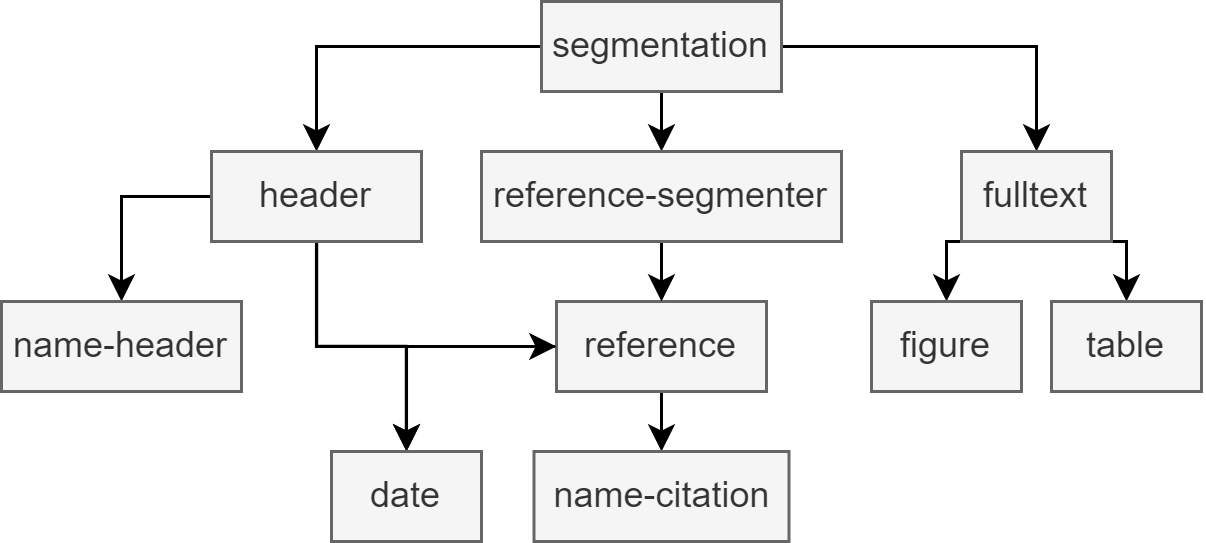
\includegraphics[width=0.7\linewidth]{images/grobid.png}
	\caption{The cascading structure of all GROBID models.}
	\label{fig:grobid}
\end{figure}

\textit{CERMINE} is an extraction system, capable of retrieving header metadata as well as reference metadata from PDF files. Similar to \textit{EXCITE} and \textit{GROBID}, the authors suggest a cascading approach using a series of different supervised and unsupervised models to enhance the performance and robustness of the overall system, allowing for more comprehensive and reliable results.\\
The extraction process starts with a layout analysis to create a hierarchical representation of a document, preserving its text content and layout features. 
Once individual characters have been retrieved, they are combined into cohesive words, followed by the assembly of lines, and ultimately integrated into zones.\\
To classify each zone accurately, a Support Vector Machine (SVM)~\cite{hearst1998support} model is employed, distinguishing between four distinct categories: metadata, body, reference, and other. 
Following the initial zone classification, a subsequent SVM model is employed to further categorize the identified zones, labeled as metadata, into distinct classes such as author zones, title zones, abstract zones, and other relevant labels.\\
Both classifiers use a wide range of geometric-based, lexical-based, sequential-based, and heuristics-based set of features. After the feature selection, the number of features is reduced to 53 and 51 features for the SVM models.\\
For the bibliography extraction, the authors employ an unsupervised approach, by clustering lines, contained in zones, into two categories, first line of a zone and other. This enables the creation of reference strings by utilizing k-means clustering~\cite{hartigan1979algorithm}. Lastly, a CRF model with additional features is used to extract all word-level zones.\\
To extract atomic metadata resulted from the header extraction as well as the bibliographic extraction, the authors propose a set of simple heuristics, which might in some cases lead to faulty label assignments. For example, first name and last name of authors are joined in an alternating order. If a reference contains multiple authors and a miss-classification occurs on the first author, the subsequent authors will be joined incorrectly, potentially rendering the complete reference unusable.\par
\textit{ParsCit}~\cite{councill2008parscit} is an open-source implementation, capable of extracting reference metadata from PDF files. In the pre-processing phase, the authors suggest heuristics to find the start and end of a reference block. The start of a block is determined, by searching for keywords, such as \enquote{References}, \enquote{Bibliography}, and \enquote{Notes} as well as lexical variations. An end of a block is determined in a similar fashion by searching for keywords signaling the end of a reference section or the end of a document.\\
To extract single reference strings, they resort to rule-based methods, employing a wide range of regular expressions. These regular expressions resolve around characteristics of different citation styles.\\
After the isolation of reference strings, a CRF model is used to classify reference token into 13 categories, such as author, date, title. Lexical-based, style-based, and heuristic-based features are used to train the CRF model.\\
The post-processing phase utilizes further heuristics to group several labels, such as names or pages, and normalize specific labels, for example, to retrieve a numeric value from the notion \enquote{vol. 5}.\\
One has to notice, that the suggested pre-processing heuristics to identify reference blocks fail, if the presented documents is written in any language other than English. The authors' further assumption that the input text is well-formed overlooks practical considerations that arise when dealing with real-world scenarios, such as the conversion of analog text into a digital format using OCR systems. In such cases, imperfections, errors, and inconsistencies can be introduced during the OCR process, making the assumption of well-formed input text unrealistic.\par
\textit{Neural ParsCit}~\cite{prasad2018neural} is an improved version of the original \textit{ParsCit} system. The authors show that the use of a BiLSTM-CRF model instead of the original CRF model can further improve the results of the extraction process.\\
Since the authors interchanged only the component responsible for reference string classification, the main concerns regarding the pre-processing phase still apply.
\newpage

\section{Software Applications}
There are several open-source tools available for reference parsing, which can be divided into two groups: standalone reference parsers, which are capable to extract metadata from blocks of references or reference strings, and tools with extended functionality, such as header metadata extraction.\\
Standalone reference parsers focus solely on parsing and extracting information from bibliographic references. These tools are specifically designed to extract metadata such as authors, titles, publication years, and journal names from reference strings:

\begin{itemize}
    \item Neural ParsCit\footnote{https://github.com/opensourceware/Neural-ParsCit}
    \item EXParser\footnote{https://github.com/exciteproject/Exparser}
    \item AnyStyle\footnote{https://github.com/inukshuk/anystyle}, based on a CRF model
    \item Reference Tagger\footnote{https://github.com/rmcgibbo/reftagger}, utilizing a CRF model
\end{itemize}

On the other hand, there are tools with wider functionality that incorporate reference parsing. These applications may offer additional features such as structure analysis or header extraction. While reference parsing is one of their functionalities, they provide a more comprehensive suite of tools for various document-related tasks. They include:

\begin{itemize}
    \item GROBID\footnote{https://github.com/kermitt2/grobid}
    \item CERMINE\footnote{https://github.com/CeON/CERMINE}
    \item ParsCit\footnote{https://github.com/knmnyn/ParsCit}
    \item PDFSSA4MET\footnote{https://github.com/eliask/pdfssa4met}, utilizes a rule-based approach
    \item Science Parse\footnote{https://github.com/allenai/science-parse}, uses a CRF model
\end{itemize}

\section{Datasets}
The dataset used to train the \textit{EXCITE} toolchain models, is a collection of various assembled smaller datasets as well as data annotated by the authors~\cite{excite_methods}.\\
It consists of self-labeled reference data from 125 annotated essays written in German and 100 articles written in English. The extracted references of English documents are, however composed of various languages. Both, English and German documents were collected from the Social Science Open Access Repository (SSOAR)~\cite{noauthor_ssoar_nodate}.\\
The authors note, that a small portion of these documents consists of grey literature, which can result in impurities in some reference strings, e.g. references without authors for organisational reports or datasets.\\
Furthermore, they integrated all reference strings from the Cermine dataset~\cite{tkaczyk2015cermine}, which is a subset of the GROTOAP2 dataset~\cite{tkaczyk2014grotoap2}.\\
Lastly, reference strings from another 100 articles, in mixed German and English language, were added from the Grobid dataset~\cite{GROBID_pref}. Their final annotated dataset contains 12,248 reference strings.\\
The Excite dataset builds the foundation of our training data for the proposed Reference Segmentation model.\par
PubMed Central (PMC) is a full-text internet archive for scientifc literature, with focus on biomedical and life sciences publications. As of 2017, PMC contained over 4 Million articles~\cite{gamble2017pubmed}.\\
The \textit{PMC Open Access Subset (PMC OAS)}~\cite{pmcoas}, a subset of articles from the PMC archive, contains over two million articles. Data included in the subset consists of the complete text of articles as well as metadata associated with each article.\\
This metadata can include information such as authors, affiliation of authors, title, publication date, and even segmented references.\\
As as subset of PMC, all articles are likewise from the domain of Bio medicine and are almost exclusively written in English.\par
The \textit{PubLayNet} dataset~\cite{zhong2019publaynet} is a large collection of document images with corresponding annotations about the layout structure of an image.\\
The dataset was automatically created and annotated utilizing the PMC OAS dataset and thus, contains mostly documents written in English.\\
Layout information consists of bounding boxes and segmented polygons. The authors distinguish between five different layout categories: text, title, list, table, and figure.\par
\textit{DocBank} is a large-scale dataset of extracted pages from articles written mostly in English, encompassing textual and layout information~\cite{li2020docbank}.\\
The dataset consists of 500,000 document pages, whereas 400,000 pages are reserved for training and 50,000 are intended for validation and testing, respectively.\\
Used data is created by employing methods based on weak supervision using the preprint Server arXiv.\\
The authors utilize the semantic structure information of the \LaTeX source code of an article to extract text, layout information, and corresponding labels.\\
For each document page exist two different files, an image file of the document and a Comma-separated values (CSV) file containing the text token and information about its bounding box, text color, font, and its assigned label. A concise overview is given in Table~\ref{tab:docbank_data}.\\
The DocBank dataset is used as a foundation for our Document Segmentation model, since its class labels contain all relevant information to extract document header metadata as well as reference metadata.\par
The \textit{balanced Wikipedia-based Annotation for Named Entity Recognition (WikiANN)} dataset is a multilingual dataset for Named Entity Recognition (NER) tasks~\cite{rahimi2019massively}.\\
It consists of short token sequences extracted from Wikipedia, as well as corresponding label for each token. The balanced WikiANN is a subset of the original WikiANN~\cite{pan-etal-2017-cross}.\\
The authors reduced the number of languages from 282 to 41 languages, utilized IOB2-tags for class labels, and balanced the distribution of class labels. NER IOB2-tags are composed of location, organisation, and person.\\
The Author Extraction model relies on the data provided by the balanced WikiANN dataset as its foundational basis.\par
The \textit{CoNLL-2003} dataset~\cite{conll2003} originates from the 2003 shared task of the Conference on Computational Language Learning. It contains data from two different corpora, an English and German collection of short sentences gathered different news sources.\\
The English corpus was created from news stories published by the international news agency Reuters. To establish the German corpus, the Frankfurter Allgemeine Rundschau was used.\\
Overall, the dataset consists of over 600,000 annotated token, evenly distributed between German and English annotated sentences. The labeled data contains part-of-speech (POS) tags, chunk tags, and NER tags for every token.\\
In comparison with the WikiANN, the NER tags are extended by on label (MISC) and it uses simple IOB-tags. Despite these small differences, both CoNLL-2003 and WikiANN are fully compatible.\\
Numerous scientific articles reference the CoNLL-2003 dataset and utilize it as benchmark dataset for NER and NER-related tasks~\cite{ner_survey}.\par
Cioffi et al.~\cite{cioffi2022structured} present a small dataset of manually annotated scientific publications. The dataset contains 56 articles from 27 different subject areas, such as computer science, physics, psychology, medicine, and social sciences. It consists of 2,538 bibliographic references from nearly 1,000 distinct journals.

\chapter{Methods}\label{chap:methods}
In this chapter, we discuss the methodology employed to develop a robust system that unifies the extraction of metadata from both article headers and references, regardless of the language in which they are written, English or German. We present our conceptual framework (Section~\ref{sec:conceptual_framework}), where we discuss our ideas and strategies aimed at addressing the research problems and how we want to solve them.\\
The chapter includes a detailed explanation of the datasets we annotated (Section~\ref{sec:methods_datasets}) and the thought process behind their creation. We discuss our intentions and considerations that guided us in assembling datasets that represent the problem domain and enable the training and evaluation of our models.\\
Furthermore, we provide insights into the models (Section~\ref{sec:methods_models}) we employed to accomplish our task of extracting metadata from scholarly literature.

\section{Conceptual Framework}\label{sec:conceptual_framework}
Upon conducting an extensive examination of available literature, software applications, and datasets related to our specific problems, we developed our conceptual framework. Our system's construction is predominantly inspired by well-regarded, peer-reviewed publications and established open-source software, namely EXParser, GROBID, CERMINE, and ParsCit. It is evident that each of these approaches employs a cascade of independently trained ML models or a combination of heuristics and ML techniques. The sequential nature of this approach introduces the risk of error propagation to downstream models and amplifies the presence of noisy or faulty input data with each passing layer.\\
However, in observing the benefits of a modular system, we found that it allows for greater flexibility in interchanging models and adapting training data as required. Consequently, we concluded that a modular system appears to be the most suitable choice. Nevertheless, we aimed to constrain the maximum depth of sequential models to minimize the propagation of uncertainty.\\
In Chapter~\ref{chap:background}, we investigated the current state-of-the-art models in the field of Natural Language Processing (NLP), with a focus on tasks related to multilingual document understanding, cross-lingual classification, and sequence labeling. Among the models we selected for utilization and testing are mBERT and XLM-RoBERTa, which are multilingual text-based models, capable of handling various languages and tasks. Additionally, we aim to incorporate LayoutXLM, a state-of-the-art multilingual model that not only considers text but also incorporates layout and visual information from documents, providing a comprehensive approach to document understanding. As a baseline comparison, we will include a CRF model, a widely used approach in related research as we discussed in Chapter~\ref{chap:related}.

\subsection{Document Segmentation Model}\label{sec:roadmap_docseg}
Our root model must possess the capability to identify relevant sections within a document, hence referred to as the Document Segmentation Model. As demonstrated by Rizvi et al.~\cite{rizvi2020hybrid}, visual information from scans can be effectively utilized for document segmentation. Therefore, we aimed to incorporate visual information into our model as well. Furthermore, our model must be able to handle both English and German corpora effectively. It should demonstrate robustness and accuracy in processing documents in both languages.\\
Considering the requirements for handling multimodal data and the utilization of visual information along with text in both English and German languages, we utilized LayoutXLM as our Document Segmentation Model for this processing step and formulated the following requirements for our Document Segmentation Dataset:
\begin{itemize}
    \item \textbf{Historical Literature:} The \textit{GEOcite} corpus consists of articles published over a period of 70 years. Ever changing citation styles, document layouts, and even vocabulary needs to be reflected in our data.
    \item \textbf{Data Representation:} As we want to employ a Multimodal Model, we need our data presented in various formats, encompassing textual content, corresponding layout information, and as digital images.
    \item \textbf{Robustness:} We want to employ a token-based sequence-to-sequence model instead of a line-based approach to account for possible errors of the OCR layout system. An example of this occurrence can be seen in Figure~\ref{fig:layout_error}.
    \item \textbf{Multilingual:} The data should consist of documents written in English and German.
    \item \textbf{Labels:} We need a minimum of two labels, one indicating header metadata and another for reference metadata. We prefer the labels to be as fine-grained as possible for an optimal extraction process.
\end{itemize}

\begin{figure}[!ht]
    \centering
    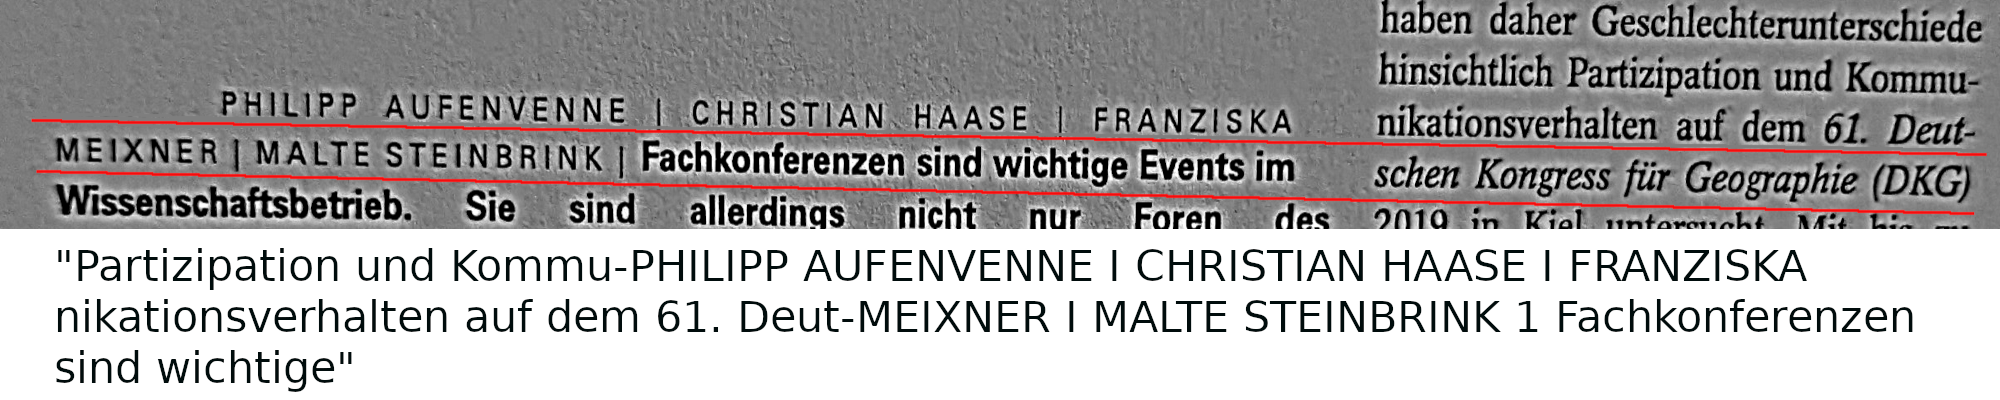
\includegraphics[width=1.0\linewidth]{images/layout_error.png}
    \caption{An example, where the layout detection of an OCR system fails. The upper part shows the detected layout, and the lower part shows the extracted text, complicating an extraction of article authors.}
    \label{fig:layout_error}
\end{figure}

We decided to utilize the DocBank dataset as the foundation for our Document Segmentation Dataset, fulfilling our requirements for robustness, data representation, and labels. To meet the historical literature and multilingual needs, we resolved to combine the DocBank dataset with an annotated dataset from the GEOcite analog corpus. Our annotated dataset was created with the intention of ensuring compatibility with the DocBank dataset in terms of output files (image, text, and layout information), format (e.g., normalized bounding boxes), and consistency of labeled data. This concatenation created a comprehensive dataset that aligns with all our requirements for fine-tuning the LayoutXLM model.

\subsection{Reference Parser Model}\label{sec:roadmap_reference_parser}
Our Document Segmentation Dataset is structured with references represented solely as word-level tokens, lacking any information about reference segments. Consequently, extracting metadata from references necessitates the use two separate models, one for reference segmentation and another for parsing the extracted reference strings.\\
To comply with our formulated robustness constraints and limit the depth of sequentially arranged models, we favored a unified approach, utilizing a single model capable in both reference segmentation and parsing. To achieve this, we fine-tuned an XML-RoBERTa model, augmented with a custom multi-output classification layer.\\
After thoroughly considering these aspects, we established the requisites for our Reference Parser Dataset:

\begin{itemize}
    \item \textbf{Domain:} The reference data in our dataset should be relevant to the domain of our corpus, particularly pertaining to the field of Geography. It should encompass specific aspects unique to the field, such as journal names and certain citation habits commonly found in Geography, such as references to local literature and newspapers.
    \item \textbf{Robustness:} Our reference strings should contain noise during training to enable the development of a robust system. By exposing the model to noisy reference data, it acquires the capacity to recover in case of errors induced from our upstream model. This deliberate inclusion of noise ensures that our parser model can withstand real-world challenges and inaccuracies, by enhancing its ability to handle variations and uncertainties in reference data.
    \item \textbf{Labels:} To support our multi-output model, we need two types of labels: a binary class to indicate whether a token marks the start of a new reference, and token-level labels for entities such as authors, titles, and journals. In addition, we need information about the start and end for each label, as they may span over multiple token.
\end{itemize}

We note, that the same requirements of \textbf{Multilingual} and \textbf{Historical Literature} as formulated in Section~\ref{sec:roadmap_docseg} also apply for this dataset. After analyzing our stated considerations, we decided to use the EXCite dataset as basis for our Reference Parser Dataset.\\
The suggested dataset utilizes a multilingual corpus and contains all the required labels. However, it does not fully meet our criteria as it includes modern Social Science articles from a broader domain, rather than from the domain of Geography itself. Furthermore, the GEOcite dataset does not encompass historical literature, which was formulated as another key requirement.\\
Given these considerations, we determined that the GEOcite dataset alone is not suitable as the basis for our Reference Parser Dataset and decided to address these limitations by annotating selected documents from our corpus and subsequently combining them with the GEOcite dataset. By doing so, we aimed to develop a comprehensive and domain-specific dataset that encompasses historical literature and fulfills all of our requirements for a sufficient Reference Parser Dataset.

\subsection{Author Parser Model}
The tokens labeled as authors from our Document Segmentation Model may also contain affiliations of the authors. Establishing citation networks relies heavily on accurately identifying the names of authors in scientific articles to link them with cited authors.\\
To accomplish this, we treat the task as a classical Named Entity Recognition (NER) problem, seeking to locate all persons mentioned in a block of text. We want to test the capabilities of mBERT, XLM-RoBERTa, and a CRF model on this task. As a result, we have formulated the following requirements for our dataset:

\begin{itemize}
    \item \textbf{Multilingual:} We want to account for language specific names and potential linguistic characteristics such as the French circumflex
    \item \textbf{Robustness:} The context in which we want to identify entities within our text block is highly constrained. To accommodate this limitation, our model should be trained on text snippets with restricted context, specifically avoiding long texts.
    \item \textbf{Labels:} We at least require a label to identify a person. However, we welcome additional labels such as organization or location, as they could potentially provide valuable information to further narrow down the author of an article.
\end{itemize}

The decision to use the WikiANN dataset as our Author Parser Dataset was driven by its unique advantages, which align well with our goals. The dataset offers a multilingual corpus, encompassing text snippets from various languages, making it suitable for evaluating the performance of our Author Parser Model on different language contexts.

\section{Datasets}\label{sec:methods_datasets}
In this section, we provide a detailed account of the methods we employed to create the datasets essential for training our models. We explore the technical aspects of the data generation process, illustrating the techniques utilized to ensure the datasets' quality and relevance. Furthermore, we address the challenges encountered during the dataset creation, discussing how we tackled various issues to achieve a comprehensive and robust training foundation for our models.

\subsection{Document Segmentation Dataset}\label{sec:document_segmentation_dataset}
Here, we present the creation process of our Document Segmentation Dataset, which serves as the foundation for training and testing our Document Segmentation Model. We outline the steps taken to obtain the data from two key sources: the GEOcite corpus and the DocBank corpus.

\subsubsection{GEOcite Corpus}
Due to the non-uniform distribution of articles across publication years in our corpus, we decided to employ a stratified sampling approach to gather the required documents. To achieve this, we divided the publication years into bins, each spanning 5 years, starting from the year 1949 until the present year. Subsequently, we sampled approximately 400 articles, ensuring an equal representation from each bin. By employing this stratified sampling method, we aim to create a dataset that is representative of the entire time span covered by our research while maintaining a balanced distribution of articles across different publication years.\\
It is our assumption that pages, with little or no information relevant to our research, would be over-represented in our dataset, since relevant metadata is expected to reside at the beginning and end of an article. With the median number of pages per article amounting to 8 pages, we expect that a considerable portion of content within each article may not directly contribute to our research objectives.\\
To address this issue, we classified the pages of an article into three distinct categories: a header page, identified by the presence of an author and title; a reference page, denoted by the presence of a reference; and a content page, recognized by the absence of author, title, and reference.\\
Next, we proceeded with the selection process, focusing on the first page of each document to extract its header page. For the identification of reference pages, we conducted a manual examination, marking all pages containing references. To ensure a balanced dataset, we sampled an equal number of pages from the reference pages, mirroring the number of header pages.\\
We further sampled an equivalent number of content pages from those that were neither designated as header nor reference pages. This comprehensive approach yielded a total of 1,365 pages, collectively forming our dataset, representative equally of the header, reference, and content pages.\\
Finally, we extracted words and bounding boxes from each page and used them to create digital images representing each page within our sample. To enhance the robustness of our overall system, we made the deliberate choice to retain irregularities and errors introduced by the OCR process. By preserving these imperfections, our system can adapt and handle real-world scenarios where OCR inaccuracies are common.\\

The annotation process for the sample was conducted using the annotation tool DataTurks~\cite{dataturks}. To ensure accuracy and consistency of our labeled data, we prepared an extensive annotation guide, documented in Appendix~\ref{chap:appendix_annotation}. This guide serves as a comprehensive reference for annotators, detailing the principles, rules, and criteria we established to achieve a well-structured and cleanly labeled dataset.\\
To streamline the annotation process for annotators, we have implemented measures for more accessibility and convenience. In addition to offering the textual representation of our sample, we provide access to PDFs and images of pages via a web server. This enables annotators to easily navigate and comprehend the context of the data they are annotating.\\

After the annotation process, we match the token labels with the corresponding token and bounding boxes. To ensure consistency with the DocBank dataset, we normalized the bounding boxes by following their proposed format, which closely resembles the format used in the MS COCO dataset~\cite{lin2014microsoft}. Here we denote coordinates of the rectangle using a tuple $(x_0, y_0, x_1, y_1)$, where $(x_0, y_0)$ corresponds to the location of the upper left corner in the bounding box, and $(x_1, y_1)$ represents the position of the lower right corner. To account for variations in resolution across transmitted images or PDFs, we employ min-max normalization to rescale the pixel values of the bounding boxes.
\begin{equation}
    x' = a + \frac{(x - \min{x})(b - a)}{\max{x} - \min{x}}
\end{equation}
This process ensures that the coordinates of the bounding boxes are adjusted to fall within a specified range of values, denoted as $[a, b]$, where $a = 0$, $b = 1000$.

\begin{table}[!ht]
	\centering
	\begin{tabular}{l|l|l|l|l|l|l|l|l|l|l}
        \textbf{Index} & \textbf{0} & \textbf{1} & \textbf{2} & \textbf{3} & \textbf{4} & \textbf{5} & \textbf{6} & \textbf{7} & \textbf{8} & \textbf{9} \\ \hline
        Content & token & $x_0$ & $y_0$ & $x_1$ & $y_1$ & R & G & B & font name & label
    \end{tabular}
	\caption{An overview about the data structure and contained layout information of the DocBank CSV file. $x_0$, $y_0$, $x_1$, and $y_1$ span the bounding box, R, G, and B yield the font color of a token.}
	\label{tab:docbank_data}
\end{table}

We saved our transformed sample as CSV files, following the same structure as the DocBank dataset, with the exception of the omitted features font and text color. Additionally, each CSV file is accompanied by a resized image with a resolution of 244 x 244 pixels. For reference, Table~\ref{tab:docbank_data} provides an overview of the data structure used in the DocBank dataset, aiding in understanding the organization and content of our dataset.\\
For testing the performance of our Document Segmentation Model, we set aside 10\% of our sampled data to create a separate test set. A comprehensive breakdown of the composition of the resulting GEOcite portion of our dataset can be examined in Table~\ref{tab:dataset_docseg_geocite}. It provides detailed insights into the distribution of different labels across the training and test set of our dataset.

\begin{table}[!ht]
\centering
\begin{tabular}{l|llllll|}
\cline{2-7}
\multicolumn{1}{c|}{}                & \multicolumn{6}{c|}{Document Segmentation Dataset - GEOcite Corpus}                                                                                                                                                                                                                                                                                                                 \\ \hline
\multicolumn{1}{|l|}{\textbf{label}} & \multicolumn{1}{l|}{\cellcolor[HTML]{DAE8FC}\textbf{train}} & \multicolumn{1}{l|}{\cellcolor[HTML]{EFEFEF}\textbf{}} & \multicolumn{1}{l|}{\cellcolor[HTML]{DAE8FC}\textbf{test}} & \multicolumn{1}{l|}{\cellcolor[HTML]{EFEFEF}\textbf{}} & \multicolumn{1}{l|}{\cellcolor[HTML]{DAE8FC}\textbf{total}} & \cellcolor[HTML]{EFEFEF}\textbf{} \\ \hline
\multicolumn{1}{|l|}{abstract}       & \multicolumn{1}{l|}{\cellcolor[HTML]{DAE8FC}35,070}         & \multicolumn{1}{l|}{\cellcolor[HTML]{EFEFEF}5.32\%}    & \multicolumn{1}{l|}{\cellcolor[HTML]{DAE8FC}5,473}         & \multicolumn{1}{l|}{\cellcolor[HTML]{EFEFEF}8.21\%}    & \multicolumn{1}{l|}{\cellcolor[HTML]{DAE8FC}40,543}         & \cellcolor[HTML]{EFEFEF}5.58\%    \\ \hline
\multicolumn{1}{|l|}{author}         & \multicolumn{1}{l|}{\cellcolor[HTML]{DAE8FC}2,347}          & \multicolumn{1}{l|}{\cellcolor[HTML]{EFEFEF}0.36\%}    & \multicolumn{1}{l|}{\cellcolor[HTML]{DAE8FC}256}           & \multicolumn{1}{l|}{\cellcolor[HTML]{EFEFEF}0.38\%}    & \multicolumn{1}{l|}{\cellcolor[HTML]{DAE8FC}2,603}          & \cellcolor[HTML]{EFEFEF}0.36\%    \\ \hline
\multicolumn{1}{|l|}{caption}        & \multicolumn{1}{l|}{\cellcolor[HTML]{DAE8FC}6,901}          & \multicolumn{1}{l|}{\cellcolor[HTML]{EFEFEF}1.05\%}    & \multicolumn{1}{l|}{\cellcolor[HTML]{DAE8FC}706}           & \multicolumn{1}{l|}{\cellcolor[HTML]{EFEFEF}1.06\%}    & \multicolumn{1}{l|}{\cellcolor[HTML]{DAE8FC}7,607}          & \cellcolor[HTML]{EFEFEF}1.05\%    \\ \hline
\multicolumn{1}{|l|}{equation}       & \multicolumn{1}{l|}{\cellcolor[HTML]{DAE8FC}31}             & \multicolumn{1}{l|}{\cellcolor[HTML]{EFEFEF}0.01\%}    & \multicolumn{1}{l|}{\cellcolor[HTML]{DAE8FC}0}             & \multicolumn{1}{l|}{\cellcolor[HTML]{EFEFEF}0\%}       & \multicolumn{1}{l|}{\cellcolor[HTML]{DAE8FC}31}             & \cellcolor[HTML]{EFEFEF}0.01\%    \\ \hline
\multicolumn{1}{|l|}{figure}         & \multicolumn{1}{l|}{\cellcolor[HTML]{DAE8FC}5,587}          & \multicolumn{1}{l|}{\cellcolor[HTML]{EFEFEF}0.85\%}    & \multicolumn{1}{l|}{\cellcolor[HTML]{DAE8FC}629}           & \multicolumn{1}{l|}{\cellcolor[HTML]{EFEFEF}0.94\%}    & \multicolumn{1}{l|}{\cellcolor[HTML]{DAE8FC}6,216}          & \cellcolor[HTML]{EFEFEF}0.86\%    \\ \hline
\multicolumn{1}{|l|}{footer}         & \multicolumn{1}{l|}{\cellcolor[HTML]{DAE8FC}36,008}         & \multicolumn{1}{l|}{\cellcolor[HTML]{EFEFEF}5.47\%}    & \multicolumn{1}{l|}{\cellcolor[HTML]{DAE8FC}4,270}         & \multicolumn{1}{l|}{\cellcolor[HTML]{EFEFEF}6.4\%}     & \multicolumn{1}{l|}{\cellcolor[HTML]{DAE8FC}40,278}         & \cellcolor[HTML]{EFEFEF}5.55\%    \\ \hline
\multicolumn{1}{|l|}{paragraph}      & \multicolumn{1}{l|}{\cellcolor[HTML]{DAE8FC}410,715}        & \multicolumn{1}{l|}{\cellcolor[HTML]{EFEFEF}62.36\%}   & \multicolumn{1}{l|}{\cellcolor[HTML]{DAE8FC}40,314}        & \multicolumn{1}{l|}{\cellcolor[HTML]{EFEFEF}60.45\%}   & \multicolumn{1}{l|}{\cellcolor[HTML]{DAE8FC}451,029}        & \cellcolor[HTML]{EFEFEF}62.18\%   \\ \hline
\multicolumn{1}{|l|}{reference}      & \multicolumn{1}{l|}{\cellcolor[HTML]{DAE8FC}142,033}        & \multicolumn{1}{l|}{\cellcolor[HTML]{EFEFEF}21.56\%}   & \multicolumn{1}{l|}{\cellcolor[HTML]{DAE8FC}13,334}        & \multicolumn{1}{l|}{\cellcolor[HTML]{EFEFEF}20\%}      & \multicolumn{1}{l|}{\cellcolor[HTML]{DAE8FC}155,367}        & \cellcolor[HTML]{EFEFEF}21.42\%   \\ \hline
\multicolumn{1}{|l|}{section}        & \multicolumn{1}{l|}{\cellcolor[HTML]{DAE8FC}4,427}          & \multicolumn{1}{l|}{\cellcolor[HTML]{EFEFEF}0.67\%}    & \multicolumn{1}{l|}{\cellcolor[HTML]{DAE8FC}380}           & \multicolumn{1}{l|}{\cellcolor[HTML]{EFEFEF}0.57\%}    & \multicolumn{1}{l|}{\cellcolor[HTML]{DAE8FC}4,807}          & \cellcolor[HTML]{EFEFEF}0.66\%    \\ \hline
\multicolumn{1}{|l|}{table}          & \multicolumn{1}{l|}{\cellcolor[HTML]{DAE8FC}10,123}         & \multicolumn{1}{l|}{\cellcolor[HTML]{EFEFEF}1.54\%}    & \multicolumn{1}{l|}{\cellcolor[HTML]{DAE8FC}692}           & \multicolumn{1}{l|}{\cellcolor[HTML]{EFEFEF}1.04\%}    & \multicolumn{1}{l|}{\cellcolor[HTML]{DAE8FC}10,815}         & \cellcolor[HTML]{EFEFEF}1.49\%    \\ \hline
\multicolumn{1}{|l|}{title}          & \multicolumn{1}{l|}{\cellcolor[HTML]{DAE8FC}5,387}          & \multicolumn{1}{l|}{\cellcolor[HTML]{EFEFEF}0.82\%}    & \multicolumn{1}{l|}{\cellcolor[HTML]{DAE8FC}638}           & \multicolumn{1}{l|}{\cellcolor[HTML]{EFEFEF}0.96\%}    & \multicolumn{1}{l|}{\cellcolor[HTML]{DAE8FC}6,025}          & \cellcolor[HTML]{EFEFEF}0.83\%    \\ \hline
\end{tabular}
\caption{The composition and amount of word-level token of the GEOcite portion of the Document Segmentation Dataset.}
\label{tab:dataset_docseg_geocite}
\end{table}

\subsubsection{DocBank Corpus}

Due to the limited size of our self-annotated data in comparison to the extensive DocBank dataset, we exercised caution in utilizing only a small portion of pages from the latter to avoid significant oversampling. To further ensure a representative sample, we adopted a stratified sampling approach, similar to that employed in the creation of the GEOcite portion of our dataset.\\
In this sampling process, we again focused on three distinct categories: header pages, reference pages, and content pages. By analyzing the token labels, we determined that a header page must contain at least one author and title label, a reference page must contain at least one reference label, and a content page must have neither an author, title, nor reference label. Overall, we sampled 500 pages from within each category.\\
We further noticed, that the DocBank dataset, being automatically generated, contains a limited number of irregularities. Some examples include malformed images of articles, article pages with only a few tokens, and faulty text encoding for word tokens. Given the constrained size of our constructed dataset, we aimed to ensure the utmost quality of our data.\\
To achieve this, we conducted a thorough search of all sampled pages and identified those with irregularities. Subsequently, we removed the pages with such anomalies and replaced them with new instances from within their respective categories.\\
Similarly to the approach used for the GEOcite corpus, we allocated 10\% of our data as a dedicated test set for evaluation purposes. Table~\ref{tab:dataset_docseg_docbank} provides a detailed visualization of the distribution of word-level tokens and labels within our dataset.

\begin{table}[!ht]
\centering
\begin{tabular}{l|llllll|}
\cline{2-7}
\multicolumn{1}{c|}{}                & \multicolumn{6}{c|}{Document Segmentation Dataset - DocBank Corpus}                                                                                                                                                                                                                                                                                                                 \\ \hline
\multicolumn{1}{|l|}{\textbf{label}} & \multicolumn{1}{l|}{\cellcolor[HTML]{DAE8FC}\textbf{train}} & \multicolumn{1}{l|}{\cellcolor[HTML]{EFEFEF}\textbf{}} & \multicolumn{1}{l|}{\cellcolor[HTML]{DAE8FC}\textbf{test}} & \multicolumn{1}{l|}{\cellcolor[HTML]{EFEFEF}\textbf{}} & \multicolumn{1}{l|}{\cellcolor[HTML]{DAE8FC}\textbf{total}} & \cellcolor[HTML]{EFEFEF}\textbf{} \\ \hline
\multicolumn{1}{|l|}{abstract}       & \multicolumn{1}{l|}{\cellcolor[HTML]{DAE8FC}56,912}         & \multicolumn{1}{l|}{\cellcolor[HTML]{EFEFEF}7.55\%}    & \multicolumn{1}{l|}{\cellcolor[HTML]{DAE8FC}6,430}         & \multicolumn{1}{l|}{\cellcolor[HTML]{EFEFEF}7.42\%}    & \multicolumn{1}{l|}{\cellcolor[HTML]{DAE8FC}63,342}         & \cellcolor[HTML]{EFEFEF}7.53\%    \\ \hline
\multicolumn{1}{|l|}{author}         & \multicolumn{1}{l|}{\cellcolor[HTML]{DAE8FC}11,318}         & \multicolumn{1}{l|}{\cellcolor[HTML]{EFEFEF}1.5\%}     & \multicolumn{1}{l|}{\cellcolor[HTML]{DAE8FC}2,136}         & \multicolumn{1}{l|}{\cellcolor[HTML]{EFEFEF}2.46\%}    & \multicolumn{1}{l|}{\cellcolor[HTML]{DAE8FC}13,454}         & \cellcolor[HTML]{EFEFEF}1.6\%     \\ \hline
\multicolumn{1}{|l|}{caption}        & \multicolumn{1}{l|}{\cellcolor[HTML]{DAE8FC}13,414}         & \multicolumn{1}{l|}{\cellcolor[HTML]{EFEFEF}1.78\%}    & \multicolumn{1}{l|}{\cellcolor[HTML]{DAE8FC}1,661}         & \multicolumn{1}{l|}{\cellcolor[HTML]{EFEFEF}1.92\%}    & \multicolumn{1}{l|}{\cellcolor[HTML]{DAE8FC}15,075}         & \cellcolor[HTML]{EFEFEF}1.79\%    \\ \hline
\multicolumn{1}{|l|}{equation}       & \multicolumn{1}{l|}{\cellcolor[HTML]{DAE8FC}28,618}         & \multicolumn{1}{l|}{\cellcolor[HTML]{EFEFEF}3.79\%}    & \multicolumn{1}{l|}{\cellcolor[HTML]{DAE8FC}1,656}         & \multicolumn{1}{l|}{\cellcolor[HTML]{EFEFEF}1.91\%}    & \multicolumn{1}{l|}{\cellcolor[HTML]{DAE8FC}30,274}         & \cellcolor[HTML]{EFEFEF}3.6\%     \\ \hline
\multicolumn{1}{|l|}{figure}         & \multicolumn{1}{l|}{\cellcolor[HTML]{DAE8FC}15,311}         & \multicolumn{1}{l|}{\cellcolor[HTML]{EFEFEF}2.03\%}    & \multicolumn{1}{l|}{\cellcolor[HTML]{DAE8FC}67}            & \multicolumn{1}{l|}{\cellcolor[HTML]{EFEFEF}0.08\%}    & \multicolumn{1}{l|}{\cellcolor[HTML]{DAE8FC}15,378}         & \cellcolor[HTML]{EFEFEF}1.83\%    \\ \hline
\multicolumn{1}{|l|}{footer}         & \multicolumn{1}{l|}{\cellcolor[HTML]{DAE8FC}4,783}          & \multicolumn{1}{l|}{\cellcolor[HTML]{EFEFEF}0.63\%}    & \multicolumn{1}{l|}{\cellcolor[HTML]{DAE8FC}576}           & \multicolumn{1}{l|}{\cellcolor[HTML]{EFEFEF}0.66\%}    & \multicolumn{1}{l|}{\cellcolor[HTML]{DAE8FC}5,359}          & \cellcolor[HTML]{EFEFEF}0.64\%    \\ \hline
\multicolumn{1}{|l|}{paragraph}      & \multicolumn{1}{l|}{\cellcolor[HTML]{DAE8FC}465,221}        & \multicolumn{1}{l|}{\cellcolor[HTML]{EFEFEF}61.7\%}    & \multicolumn{1}{l|}{\cellcolor[HTML]{DAE8FC}55,610}        & \multicolumn{1}{l|}{\cellcolor[HTML]{EFEFEF}64.2\%}    & \multicolumn{1}{l|}{\cellcolor[HTML]{DAE8FC}520,831}        & \cellcolor[HTML]{EFEFEF}61.96\%   \\ \hline
\multicolumn{1}{|l|}{reference}      & \multicolumn{1}{l|}{\cellcolor[HTML]{DAE8FC}146,663}        & \multicolumn{1}{l|}{\cellcolor[HTML]{EFEFEF}19.45\%}   & \multicolumn{1}{l|}{\cellcolor[HTML]{DAE8FC}17,462}        & \multicolumn{1}{l|}{\cellcolor[HTML]{EFEFEF}20.16\%}   & \multicolumn{1}{l|}{\cellcolor[HTML]{DAE8FC}164,125}        & \cellcolor[HTML]{EFEFEF}19.53\%   \\ \hline
\multicolumn{1}{|l|}{section}        & \multicolumn{1}{l|}{\cellcolor[HTML]{DAE8FC}3,990}          & \multicolumn{1}{l|}{\cellcolor[HTML]{EFEFEF}0.53\%}    & \multicolumn{1}{l|}{\cellcolor[HTML]{DAE8FC}402}           & \multicolumn{1}{l|}{\cellcolor[HTML]{EFEFEF}0.46\%}    & \multicolumn{1}{l|}{\cellcolor[HTML]{DAE8FC}4,392}          & \cellcolor[HTML]{EFEFEF}0.52\%    \\ \hline
\multicolumn{1}{|l|}{table}          & \multicolumn{1}{l|}{\cellcolor[HTML]{DAE8FC}4,396}          & \multicolumn{1}{l|}{\cellcolor[HTML]{EFEFEF}0.58\%}    & \multicolumn{1}{l|}{\cellcolor[HTML]{DAE8FC}261}           & \multicolumn{1}{l|}{\cellcolor[HTML]{EFEFEF}0.3\%}     & \multicolumn{1}{l|}{\cellcolor[HTML]{DAE8FC}4,657}          & \cellcolor[HTML]{EFEFEF}0.55\%    \\ \hline
\multicolumn{1}{|l|}{title}          & \multicolumn{1}{l|}{\cellcolor[HTML]{DAE8FC}3,326}          & \multicolumn{1}{l|}{\cellcolor[HTML]{EFEFEF}0.44\%}    & \multicolumn{1}{l|}{\cellcolor[HTML]{DAE8FC}361}           & \multicolumn{1}{l|}{\cellcolor[HTML]{EFEFEF}0.42\%}    & \multicolumn{1}{l|}{\cellcolor[HTML]{DAE8FC}3,687}          & \cellcolor[HTML]{EFEFEF}0.43\%    \\ \hline
\end{tabular}
\caption{The composition and amount of word-level token of the DocBank portion of the Document Segmentation Dataset.}
\label{tab:dataset_docseg_docbank}
\end{table}

Finally, the two portions of the dataset, the DocBank corpus and the self-annotated data from the GEOcite corpus, are joined to create the Document Segmentation Dataset. This unified dataset comprises resized images, along with corresponding tokens and bounding boxes. In total, the dataset contains 2,579 instances for training and 286 instances for testing.

\subsection{Reference Parser Dataset}
The EXCite dataset, which we use as foundation of the Reference Parser Dataset, contains one XML file per document, where each line in this document resembles one reference string. The different entities are enclosed with XML tags, resembling their label. Figure~\ref{fig:reference_xml} illustrates the exact structure of the EXCite dataset.\\
The existing split of the training and test sets in the EXCite dataset is conducted at the document level rather than considering the overall number of reference strings. While this approach may lead to an unbalanced distribution of training and test instances due to potential sampling variations, we made the decision to follow the same document-level split for our labeled data. This choice ensures that the ratio of training and test documents aligns with that of the EXCite dataset, enabling us to maintain a coherent dataset.

\begin{figure}[!ht]
    \centering
    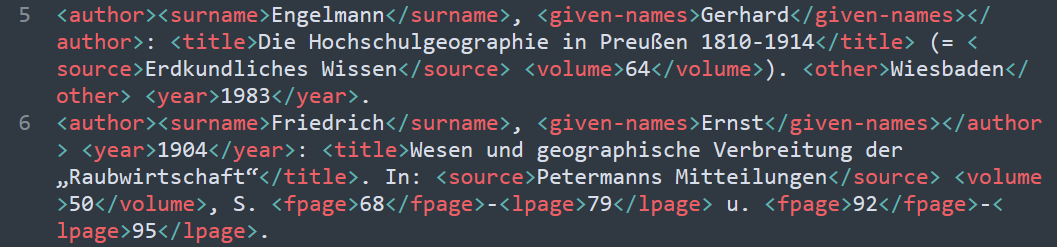
\includegraphics[width=0.95\linewidth]{images/example_reference_xml.png}
    \caption{The contents of an XML file from the GEOcite dataset.}
    \label{fig:reference_xml}
\end{figure}

As previously described in Section ~\ref{sec:document_segmentation_dataset}, we employed a stratified sampling approach based on the historic distribution of articles. This method yielded a collection of 188 documents.\\
Subsequently, we extracted the text layer from the obtained PDF files to prepare the data for annotation and decided, following our principle of robustness, to keep potential errors induced by the OCR process.\\

To accomplish the annotation process, we utilized the EXRef-Identifier, an annotation tool that is part of the EXannotator incorporated in the EXCITE toolchain, integrated in the EXCITE toolchain.\\
In the initial annotation step, we focused on extracting and segmenting references from our sample literature. The output files generated from this process were subsequently fed into a second annotation tool called EXRef-Segmentation. This second tool was utilized to identify and annotate specific entities within each reference string, including author names, titles, publication dates, and journal information.\\
This process resulted in 5,073 annotated reference strings from the GEOcite corpus, totaling the cumulative amount of reference strings to 17,569.\\

Next, we extracted token-strings and converted XML-tags of each entity to IOB2-tags. New lines indicate a new reference, which we use to label the first token-string of each line as beginning of a reference, all other token-strings are labeled as intermediate in this regard.\\
Note, that we do not yet use word-level token at this step, as the further tokenization process is dependent on the used tokenizer and employed model. In Table~\ref{tab:reference_segmented}, we present a comprehensive illustration of the resulting token-strings and their corresponding labels.\\
We will explain in detail, how we construct our atomic training and test instances, tokenization, and how this approach will aid in a robust training in Section~\ref{sec:component_ref_parser}.

\begin{table}[!ht]
    \centering
    \begin{tabular}{|l|l|l|l|}
        \hline
        \textbf{token-string} & \textbf{entity IOB} & \textbf{entity label} & \textbf{segment IOB} \\ \hline \hline
        Engelmann & B & author & B \\ \hline
        ,  & I & author & I \\ \hline
        Gerhard & I & author & I \\ \hline
        : & O & O & I \\ \hline
        Die Hochschulgeo(...) & B & title & I \\ \hline
        ( & O & O & I \\ \hline
        Erdkundliches Wissen & B & source & I \\ \hline
        , & O & O & I \\ \hline
        64 & B & volume & I \\ \hline
        ). & O & O & I \\ \hline
        Wiesbaden & B & other & I \\ \hline
        , & O & O & I \\ \hline
        1983 & B & year & I \\ \hline
        . & O & O & I \\ \hline
    \end{tabular}
    \label{tab:reference_segmented}
    \caption{An exemplary structure of the Reference Parser Dataset. The \textit{entity IOB} and \textit{entity label} together form IOB-labels, e.g. B-author or I-author. The \textit{segment IOB} label indicates the beginning of a new reference.}
\end{table}

After generating the CSV files containing the token-strings and labels, we proceed to split them into training and test sets, ensuring the same training and test split ratio as the GEOcite dataset. By maintaining this consistency, the concatenation of the GEOcite documents and our self-annotated documents results in a combined total of 373 training documents and 50 test documents, forming the Reference Parser Dataset.\\
An overview of all employed labels of our datasets can be seen in Table~\ref{tab:datasets_label}.

\begin{table}[!ht]
	\centering
	\begin{tabularx}{\textwidth}{l|l|X}
        \textbf{Dataset} & \textbf{Model} & \textbf{Labels}\\ \hline
        DocBank & Document Segmentation & \textit{abstract, author, caption, date, equation, figure, footer, list, paragraph, reference, section, table, title}\\\hline
        EXCITE & Reference Parser & \textit{publisher, first page, last page, title, url, author, author surname, author given-name, volume, source, editor, identifier, year, issue, other}\\\hline
        WikiANN & Author Parser & \textit{person, organisation, location}\\ \hline
    \end{tabularx}
	\caption{The utilized datasets as foundations for our models and their class labels.}
	\label{tab:datasets_label}
\end{table}

\section{Component Models}\label{sec:methods_models}
In this section, we provide a detailed exposition of the proposed modular component models, which build the foundation of our overall system. We address the intricate aspects of our methodology, covering explicit training sample generation, tokenization techniques, selection of hyperparameters, and the overall process of each of our component models' training.

\subsection{Document Segmentation Model}\label{sec:doc_model}
Many large transformer models are limited in their maximum number of input tokens, due to the use of their self-attention mechanism~\cite{vaswani2017attention} to capture long-term dependencies between all inputs of a sequence~\cite{devlin2019bert,liu2019roberta,sanh2019distilbert}. The quadratic complexity of Transformers with respect to its input sequence length, forces most model architectures to fix the length of their input sequence~\cite{wang2020linformer}.\\
While this limitation is acceptable for some applications, such as document classification or sentiment analysis, where a section of a text might suffice, sequence-to-sequence problems require the whole input length.\\
The LayoutXLM model is also constrained by these limitations, but our focus lies on classifying the entire set of tokens in a document. This emphasis results from the observation that reference sections can sometimes begin in the lower part of an article. As a result, we cannot rely solely on fixed-length single instances per page during our model fine-tuning, as they may lead to the exclusion of crucial information present in the lower sections.\\
To overcome this challenge, we decided to slice our dataset into snippets, each consisting of the maximum allowed model length of 512 tokens. In order to avoid worst-case scenarios, where a document with, for example, 513 tokens would be split into two parts of 512 token and 1 token respectively, we adopted the strategy of dividing the token per document into equal-length parts.\\

Our bounding boxes were already normalized during the dataset creation. The extracted images have the correct dimensions, but we converted them to BGR images in the preprocessing phase for our model fine-tuning, since the visual backbone expects this byte-order of color channels.\\
The tokenization was conducted utilizing a SentencePiece tokenizer~\cite{kudo2018sentencepiece} using the byte-pair-encoding subword algorithm~\cite{sennrich2016neural}. To comply with the maximum length by our model, we used padding for input token sequences. Sequences that are shorter than the maximum length, were filled in with a special $<pad>$ token. The start and end of a sequence are marked with the special token $<s>$ and $</s>$.\\
Since the position embedding layer for bounding boxes is concatenated with the text embedding layer, LayoutXLM utilizes a special empty position embedding $box_{PAD}$ aligning with all special token of the text embedding layer.\\
In our approach, subwords were not individually labeled, and we assigned them the value of -100. This value is utilized by PyTorch during the loss calculation. When computing the loss, PyTorch ignores the weights of subwords with this assigned value, effectively excluding them from contributing to the loss calculation.\\
As evident in Table~\ref{tab:dataset_docseg_geocite} and Table~\ref{tab:dataset_docseg_docbank}, we observed a highly imbalanced distribution of word-level tokens in our dataset. For instance, the majority class \textit{'paragraph'} accounts for approximately 62\% of all word-level tokens. To address potential bias towards highly frequent classes, we designed a weight vector with weights inversely proportional to their class frequencies. These weights are utilized during our model training to appropriately scale the loss function, ensuring a more balanced learning process and fair treatment of all classes.\\
Our hyperparameters, which we are trying to tune are the
\begin{itemize}
    \item learning rate: one of three values $[1e-5, 5e-5, 1e-4]$
    \item batch size: one of two values $[4, 8]$
    \item warm-up ratio: one of two values $[0, 0.1]$
\end{itemize}

Due to the split of pages into multiple samples, we ended up with multiple training instances representing the same page. To address the risk of overfitting, we limited the maximum number of training epochs to 2.\\
We conducted a 5-fold cross-validation on our training set to find our optimal model parameters. The best hyperparameters were used to fine-tune the LayoutXLM model on our whole training set and evaluated against our test set. Due to the aforementioned class imbalances we evaluate our model using the F1-score.

\subsection{Reference Parser Model}\label{sec:component_ref_parser}
As highlighted in Section~\ref{sec:roadmap_reference_parser}, one of our key objectives was to train the Reference Parser Model in a robust manner. The model receives its input tokens from the Document Segmentation Model upstream, which might contain noisy data due to the challenges of OCR and document segmentation.\\
Through our research, we have found that most existing tools and approaches use individual reference strings as input for their respective parser models to extract the required metadata. However, we opted for a slightly different approach, by feeding multiple reference strings into our model to extract atomic label from a broader context.\\
The core concept behind our proposed method is to train the model using fixed-size snippets of composite reference strings originating from the same document. These snippets can contain multiple reference strings and begin and end at random positions within a reference string.\\
Our goal is to provide diverse and contextually rich input to the model, enabling it to recover from faulty input more easily and learn within its given context. By exposing the model to varied snippets, it gains a better understanding of reference string structures and can make more accurate metadata extraction decisions, even in the presence of noisy data.\\
To accommodate the model's requirement to predict two outputs, the atomic label and the token indicating the start of a new reference, we implemented a custom classification layer and adapted the loss function to incorporate both predictions during model training. We add two linear layers connected to the last hidden layer resembling the output sequence.\\
The new loss function is the sum of the cross entropy between the entity targets (author, title, year, etc.)   and binary cross entropy is defined as
\begin{equation}
    \ell(x,y) = \ell_A(x_A,y_A) + \alpha \cdot \ell_B(x_B, y_B)
\end{equation}
with
\begin{equation}
    \ell_A(x_A,y_A) = \{l_{A_{1}},...,l_{A_{N}}\}^T, l_{A_{n}} = -w_{y_{A_{n}}} log\frac{\exp(x_{A_{n,y_{n}}})}{\sum_{c=1}^{C}\exp(x_{A_{n,c}})}
\end{equation}
\begin{equation}
    \ell_B(x_B,y_B) = \{l_{B_{1}},...,l_{B_{N}}\}^T, l_{B_{n}} = -w_{B_{n}} [y_{B_{n}} \cdot \log x_{B_{n}} + (1 - y_{B_{n}}) \cdot \log(1 - x_{B_{n}})] 
\end{equation}

where $x$ is the input, $y$ is the target, $C$ is the number of classes, and $N$ spans the minibatch dimension.\\
$\ell_A(x_A,y_A)$ is the cross entropy loss of our entity targets (author, title, year, etc.) with its input $x_A$, target $y_A$, and weight $w_A$. $\ell_B(x_B,y_B)$ is the binary cross entropy loss indicating a new reference with its corresponding input $x_B$, target $y_B$, and weight $w_B$. $\alpha$ is a parameter in the range $[0,1]$ to adjust, for emphasising one of the two outputs.\\
Given that our Reference Parser Dataset comprises token-strings instead of word-level tokens, we further preprocessed and pretokenized our data. This pretokenization involved splitting tokens based on white-spaces, digits, and specific punctuation marks such as ".", ":", ",", ";", "/", "-", "(", and ")".\\
To ensure comprehensive evaluation, we generated training and testing slices from the pretokenized data. This resulted in 2,047 training slices and 247 test slices.\\
Since the model we fine-tune, XLM-RoBERTa, also utilizes SentencePiece for tokenization, the further tokenization process is similar as described in Section~\ref{sec:doc_model}. An exemplary slice of the final dataset used for fine-tuning and testing of our model can be seen in Table~\ref{tab:ref_parser_sliced_output}.

\begin{table}[!ht]
    \centering
    \begin{tabular}{|l|l|l|}
    \hline
        \textbf{Token} & \textbf{IOB entity} & \textbf{IOB reference} \\ \hline
        \_Baden & B-other & I-ref \\ \hline
        \_- & I-other & I-ref \\ \hline
        \_Baden & I-other & I-ref \\ \hline
        \_: & O & I-ref \\ \hline
        \_No & B-publisher & I-ref \\ \hline
        mos & -100 & I-ref \\ \hline
        \_. & O & I-ref \\ \hline
        \_Drake & B-author & B-ref \\ \hline
        \_W & I-author & I-ref \\ \hline
        \_. & I-author & I-ref \\ \hline
        \_J & I-author & I-ref \\ \hline
        \_. & I-author & I-ref \\ \hline
        \_( & O & I-ref \\ \hline
        \_2005 & B-year & I-ref \\ \hline
    \end{tabular}
    \caption{An example of a reference string slice, used for fine-tuning our Reference Parser Model.}
    \label{tab:ref_parser_sliced_output}
\end{table}

The hyperparameters we are fine-tuning
\begin{itemize}
    \item learning rate:  $[1e-5, 5e-5, 1e-4]$
    \item batch size: $[4, 8, 16]$
    \item epochs: $[1-3]$
\end{itemize}
were evaluated on a 5-fold crossvalidation. Afterwards we trained our model with the best performing parameters on our whole training set. As evaluation metric we used the proposed method, focusing on text chunking, introduced on the CoNLL-2000 shared task~\cite{tjong-kim-sang-buchholz-2000-introduction}.

\subsection{Author Parser Model}
In our analysis, we observed that certain journals commonly print author names in uppercase letters only, as evident in Figure~\ref{fig:layout_error}. However, depending on the tokenization algorithm used, this practice can result in significantly different representations of an author's name. For instance, the name \enquote{Aufenvenne} could be split into 'AU', '\#\#F', '\#\#EN', '\#\#VE', '\#\#N', '\#\#NE' as uppercase and 'auf', '\#\#en', '\#\#ven', '\#\#ne' as lowercase. This discrepancy may lead to completely different word embeddings.\\
Due to potential character misclassifications of the OCR system, such as between uppercase and lowercase 'I' characters, we made a deliberate decision to use an uncased multilingual BERT model. Despite uppercase letters being a strong indicator for identifying person names, opting for an uncased model allows for a more consistent and robust extraction of author names across all journals in our corpus.\\

We combined the four parts of the wikiAnn dataset by interleaving them, resulting in a unified training and test set of text sequences in German, English, French, and Spanish. For each language, we obtained 20,000 training samples and 10,000 test samples.\\
To preprocess the dataset, we tokenized it using a word-piece tokenizer and padded the input token sequences. For sequences shorter than the maximum length supported by our chosen BERT model, we used a special $[PAD]$ token to fill in the remaining positions. To indicate the start and end of each sequence, we used the special tokens $[CLS]$ and $[SEP]$, respectively.\\
As in our previous component models, subwords were not labeled.\\
The hyperparameters we are fine-tuning are
\begin{itemize}
    \item learning rate:  $[1e-5, 5e-5, 1e-4]$
    \item batch size: $[8, 16]$
    \item epochs: $[1-3]$
\end{itemize}
As in the previous models, we conducted a 5-fold cross-validation on our training set to find our optimal model parameters.

\section{Used Software and Tools}
We used the Annotation tools DataTurks~\cite{dataturks} and EXannotator~\cite{excite_toolchain} to generate the labels for our datasets. We further used the base LayoutXML~\cite{hug_layoutxlm}, base XML-RoBERTa~\cite{hug_xlmr}, multilingual uncased~\cite{hug_uncased_bert} and cased BERT~\cite{hug_cased_bert} models from the data science platform Hugging Face~\cite{wolf2019huggingface}.
% !TeX spellcheck = en_US
% !TeX encoding = UTF-8
\chapter{BiBEx}\label{chap:bibex}

In this chapter, we present our unified system, BiBEx, which employs a cascade of ML models to extract both header and reference metadata from scientific publications. We will explain the design and architecture of our system (Section~\ref{sec:bibex_architecture}), providing insights into its underlying structure and functionality. Furthermore, we will introduce two user-friendly applications, BiBEx-UI and BiBEx-Model, that we developed to enable a efficient metadata extraction process.
Throughout this chapter, we will provide a comprehensive explanation of the workflow employed by BiBEx (Section~\ref{sec:bibex_workflow}). This will encompass the step-by-step process of how the system handles document segmentation, reference parsing, and author extraction.

% In this chapter we will introduce our unified system, BiBEx, comprising of a cascade of ML models to extract header and reference metadata. We will explain the design and architecture of our system (Section~\ref{sec:bibex_architecture}), and describe the two applications, we developed to enable a fast and user-friendly extraction process. We will also in detail explain the workflow of our system.

\section{BiBEx Architecture}\label{sec:bibex_architecture}
In order to maintain a clear separation between the User Interface and the business logic, we have developed two distinct applications. The first application, BiBEx-Model, is responsible for handling the computational logic, by processing and extracting relevant information from scientific articles utilizing our proposed ML models.\\
Meanwhile, the second application, BiBEx-UI, is designed to present visualizations of the extracted data to the user in a user-friendly manner.\\
While both solutions are designed as an ensemble of separated Web-Applications, BiBEx-Model can function as a standalone application. By utilizing its API, an user can time-efficiently query a large set of scientific literature for metadata extraction.\\
When combined, these two applications form our proposed unified Application: BiBEx.

\subsection{BiBEx-UI}\label{sec:bibex_ui}

BiBEx-UI is a user-friendly web application implemented using Vue.js~\cite{vuejs} and designed to simplify the extraction of metadata from articles for its users. It accepts input in various formats, including PDFs, scans, and raw reference text. The primary objective of BiBEx-UI is to enhance the user experience by offering an intuitive, simple, and easy-to-use interface.\\
The application further communicates with the BiBEx-Model REST API to process the input data and extract the relevant metadata. It handles all asynchronous data transfers and ensures smooth communication between the user interface and the model application.\\
In addition to its data processing capabilities, BiBEx-UI functions as visualization tool to present the results of the metadata extraction.
\newpage

\begin{figure}[!ht]
	\centering
	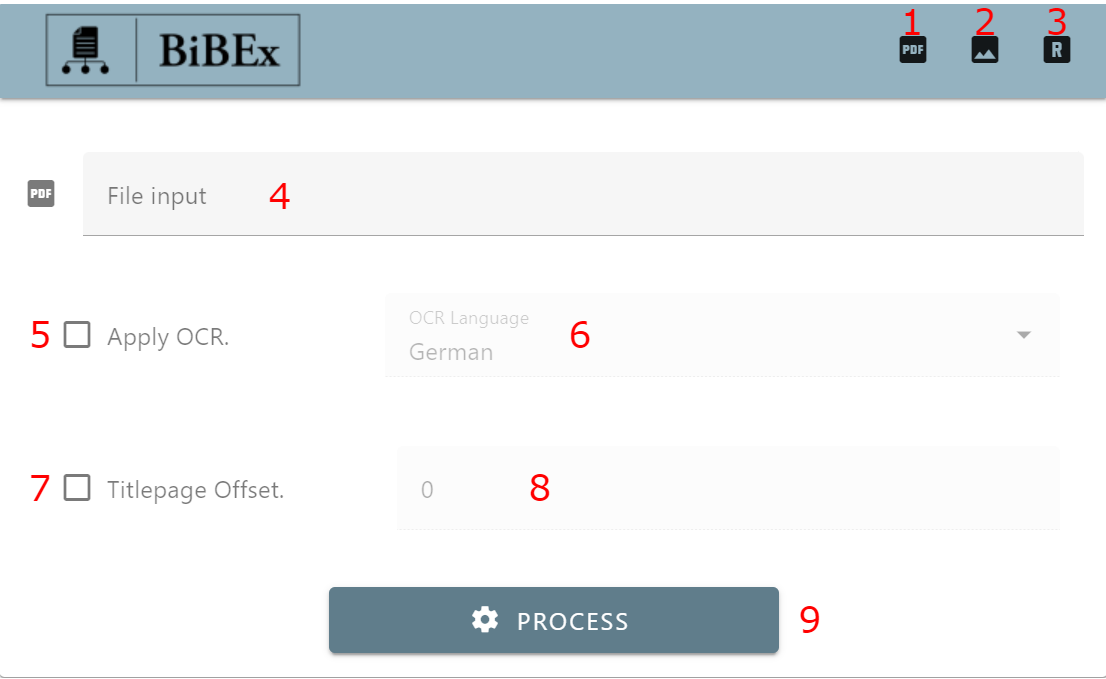
\includegraphics[width=1.0\linewidth]{images/bibex_ui.png}
	\caption{The BiBEx-UI Application provides users the capability to process their data in various forms.}
	\label{fig:bibex_ui}
\end{figure}

Figure~\ref{fig:bibex_ui} presents an exemplary overview of the User Interface for PDF data input. The UI consists of the following elements:
\begin{itemize}
    \item \textbf{[1-3]}: Mode Navigation, where an user can select between the preferred input methods as PDF \textbf{[1]}, image \textbf{[2]}, or raw reference text \textbf{[3]}.
    \item \textbf{[4]}: File Input, where the user can select a PDF file.
    \item \textbf{[5-6]}: OCR module, where the user can decide if OCR should be applied \textbf{[5]} to a PDF file and choose the language \textbf{[6]}.
    \item \textbf{[7-8]}: Titlepage offset, where an user can change the page, if desired \textbf{[7]}, which the BiBEx will use as header page \textbf{[8]}.
    \item \textbf{[9]}: Process button, where the user can start the metadata extraction process \textbf{[9]}.
\end{itemize}
\newpage

After the user clicks the \textit{Process} button, an asynchronous request is sent to the BiBEx-Model application. Subsequently, the user is redirected to a result page or, in case of unexpected behaviour, will get a dialog with an error message. The result page visualizes all relevant entities of the header extraction and the reference extraction. Moreover, users have the option to download the displayed data for their convenience. Figure~\ref{fig:bibex_output} shows a successful extraction response, visualized by the BiBEx-UI.

\begin{figure}[!ht]
	\centering
	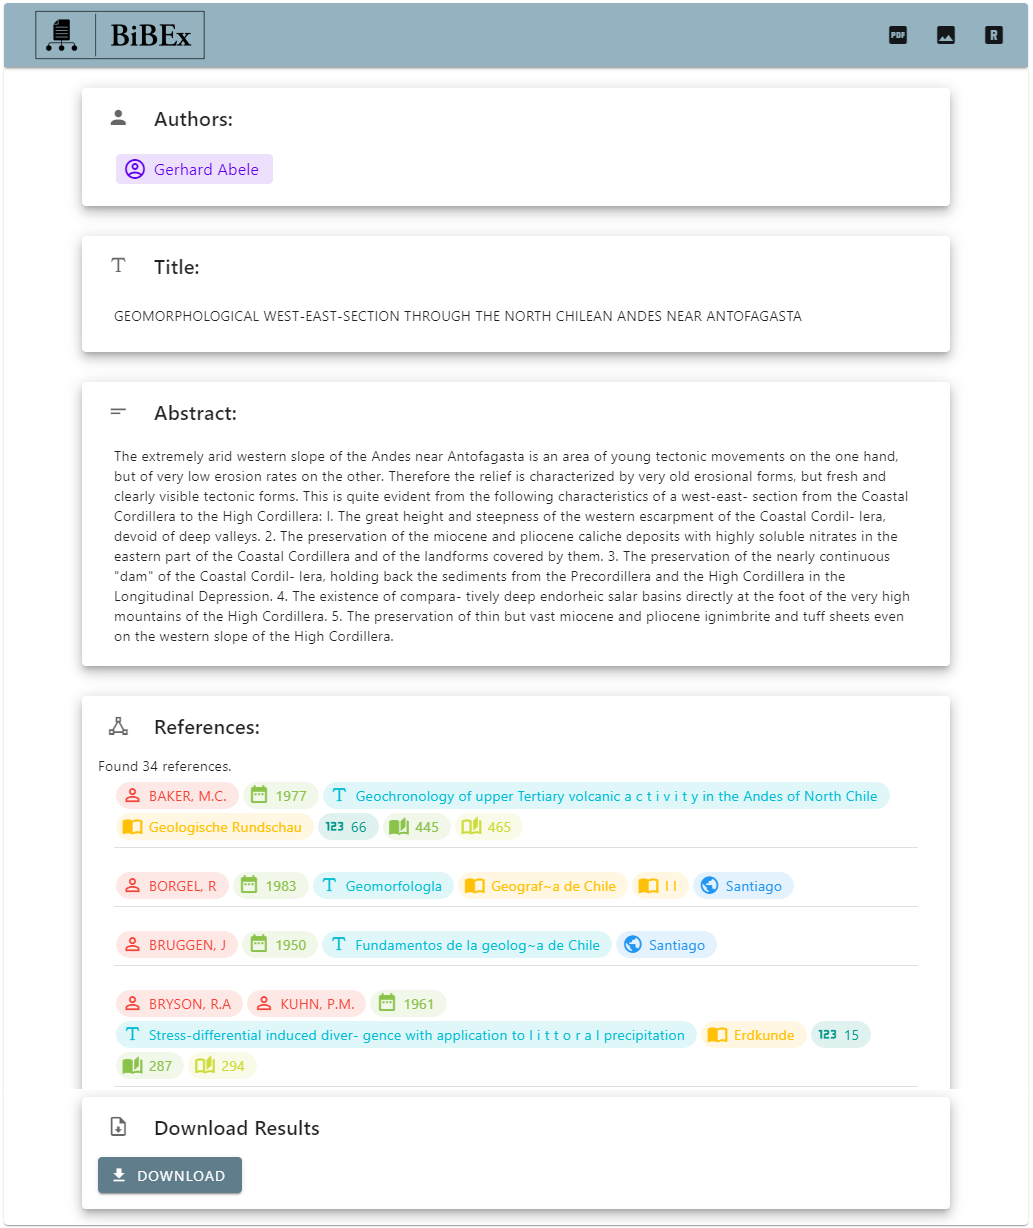
\includegraphics[width=0.7\linewidth]{images/bibex_output.png}
	\caption{The resulting output of a successful extraction process, showcased in the BiBEx-UI application.}
	\label{fig:bibex_output}
\end{figure}

\subsection{BiBEx-Model}

At its core, BiBEx-Model serves as a web application that manages the data and logic involved in the metadata extraction process. It can operate as a standalone application, allowing users to utilize its capabilities independently from BiBEx-UI, enabling swift processing of articles.\\
The application provides a REST API, developed using the FastAPI framework~\cite{fastapi}, offering three distinct endpoints resembling the different input methods.

\section{BiBEx Workflow}\label{sec:bibex_workflow}
In this section we will explain the detailed workflow of the BiBEx system, how our component models are utilized and differ during inference, and how we extract the desired metadata from publications. To offer a comprehensive understanding, we will explore all relevant system components showcased in Figure~\ref{fig:bibex_workflow}, highlighting their roles and interactions within the system.

\begin{figure}[!ht]
	\centering
	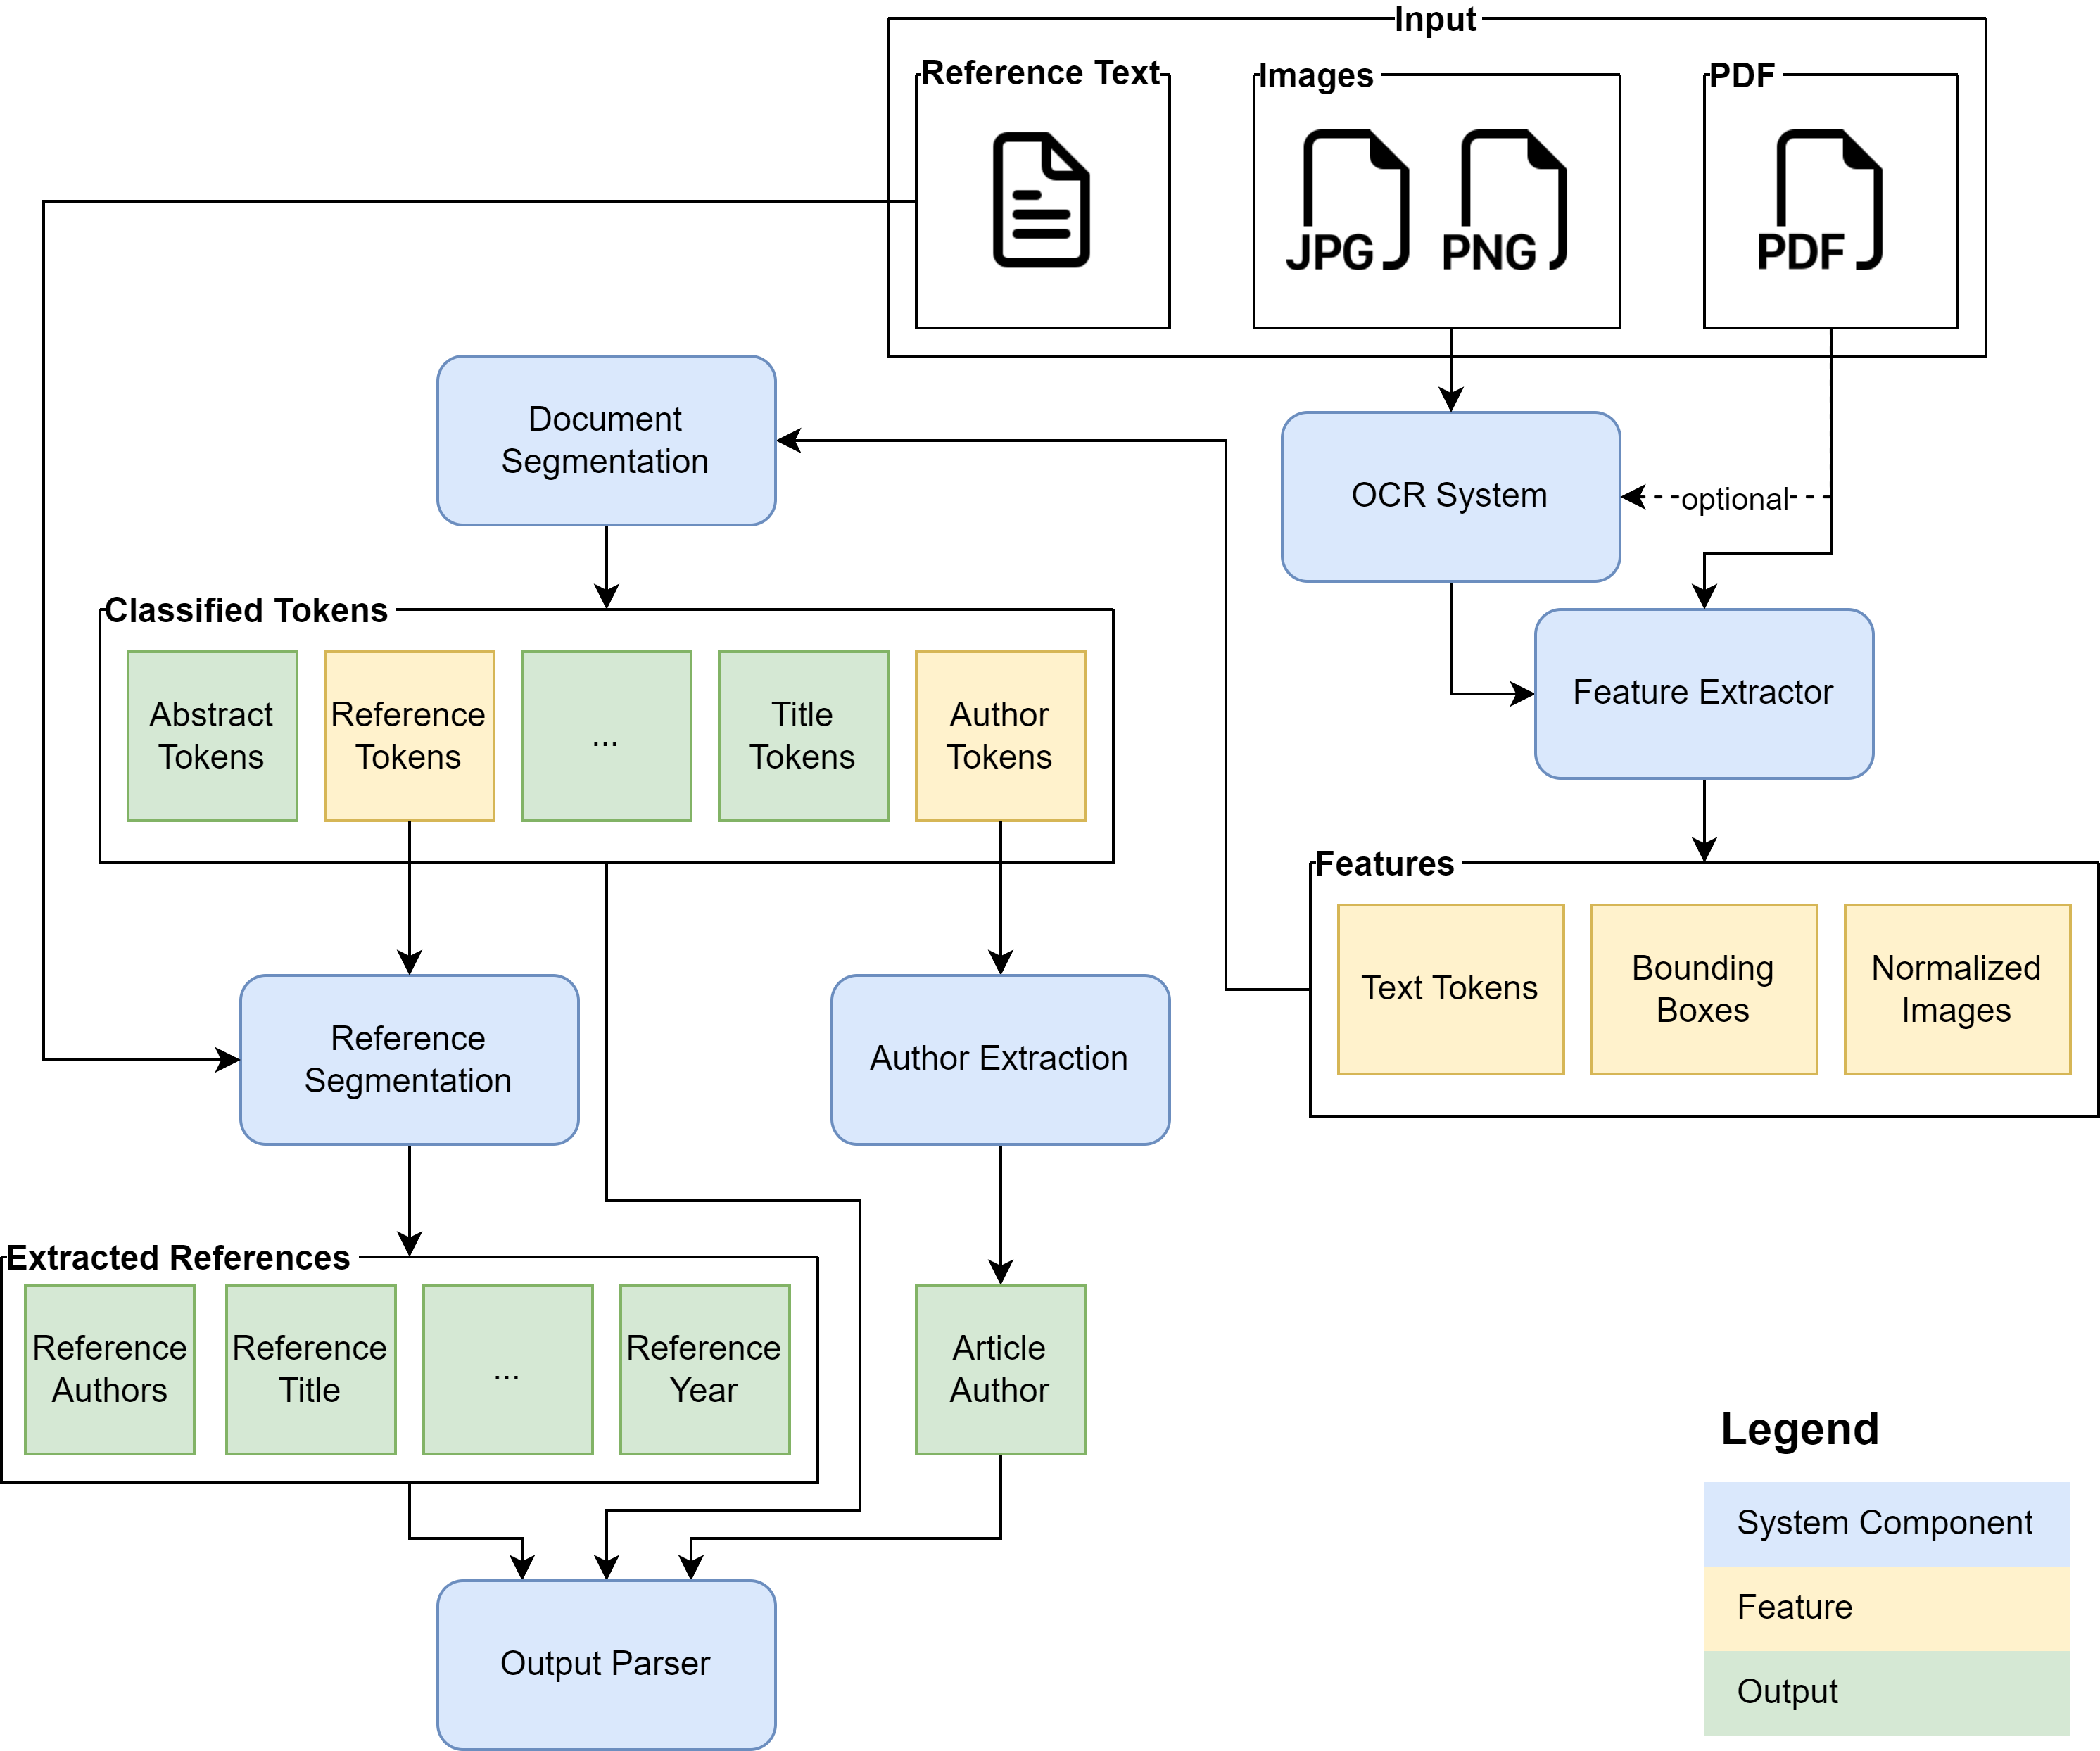
\includegraphics[width=0.7\linewidth]{images/bibex_architecture.png}
	\caption{An conceptual overview of the BiBEx workflow.}
	\label{fig:bibex_workflow}
\end{figure}

\subsection{Data Input}
As described in Section~\ref{sec:bibex_ui}, BiBEx accepts three different ways to input data as user, as PDF, PNG/JPEG images, and as plain text.

\subsection{OCR System}
We utilize the pytesseract~\cite{pytess} Python wrapper of the Tesseract Open Source OCR Engine~\cite{tesseract} to extract text from scanned images. For PDF files, this extraction step is optional, as long as the uploaded file contains a valid text layer. Furthermore, users have the flexibility to choose between English, German, French, and Spanish Tesseract language models, depending on the predominant language used in the scientific publication being processed.
\subsection{Feature Extractor}\label{sec:bibex_feature}
This System Component is responsible for further preprocessing the data and extracting features for the Document Segmentation model. As the first step, it generates normalized BGR images of all pages, ensuring consistent color representation and reducing variations across different documents. These images are resized to a standardized dimension of 224x224 pixels, resulting in a tensor shape of $(b,c,x,y)$, where $b$ denotes the batch size, $c$ the number of channels with $c=3$, $x$ the width, and $y$ the height of an image with $x=y=224$.\\
Next, we extract all word tokens and the corresponding bounding box of each token. We use the same pretrained SentencePiece tokenizer, as during our model training, which has a maximum sequence length of 512 token. In case the sequence length is below this maximum, we pad it to reach the maximum input length required by the model. Conversely, if the sequence length exceeds the tokenizer's maximum allowed length, we truncate the exceeding token.\\
Any overflowing token sequence is tokenized following the same process. The difference between the fine-tuning of our model and inference is, that we use a stride parameter of 32 token on the overflowing token to provide additional context from the previous sequence for subsequent token sequences.\\
The resulting feature set consists of tensors for input ids and attention mask, both with a dimension of $(p, b, s)$, denoting the number of pages in a transmitted article $p$, the batch size $b$, and the sequence length $s$. Additionally, bounding boxes are incorporated with a shape of $(p, b, s, 4)$, providing spatial information. Complementing these is the image tensor, which has a shape of $(p, b, c, x, y)$. Here, $p$ represents the number of pages, $b$ signifies the batch size, $c$ represents the number of image channels (set to 3), and $x$ and $y$ correspond to the width and height, respectively, of the image, both measuring 224 pixel.\\
For text layer extraction from PDFs we are using the Python package PyMuPDF~\cite{pymupdf}. For image extraction from PDF files and image conversions we utilize Pillow~\cite{clark2015pillow}.

\subsection{Document Segmentation}\label{sec:bibex_doc_seg}
The resulting batch encodings are then passed through our Document Segmentation Model, which is our fine-tuned LayoutXLM model.\\
To facilitate further processing, the model output is flattened, transforming the hierarchical representation into a sequential format. Subword token and corresponding inferred class-labels are transformed back to word-level token and labels, to pass relevant token forward to their next processing models.\\
Since we are only interested in the labels \textit{author}, \textit{reference}, and to a lesser degree \textit{title} and \textit{abstract}, we discard all other labels. Subsequent word-level token labeled as \textit{title} and \textit{abstract} are chunked together to build coherent text blocks.

\subsection{Reference Segmentation}
During this step, we focus on segmenting and parsing all tokens that have been labeled as \textit{reference} by our Document Segmentation Model. We process these tokens even if they do not form coherent text blocks, such as in cases with alternating labels or jumps between reference blocks. The idea is to extract the relevant metadata from the identified references, regardless of their arrangement.\\
The difference between fine-tuning and the production stage is, that we also use a stride parameter of 32 token as in Section~\ref{sec:bibex_feature}, taking previous context into consideration. We further utilize the whole length of our model of 512 token and do not limit our input sequence as in the training stage.\\
We utilize our Reference Parser Model with a custom pipeline, resulting in a list of grouped parsed references with the predicted entities, the textual representation, as well as start and end indices of these entities.

\subsection{Author Extraction}
In this stage, our focus lies on extracting the authors of a document. To achieve this, we treat the input again as a sequence of pretokenized token, regardless of their arrangement. We employ our Author Parser Model to extract all authors, without utilizing the stride parameter, as the number of tokens labeled as \textit{author} is unlikely to exceed our limit of 512 tokens.\\
To extract the first name and surname of document authors, as well as authors and editors from references, we employed heuristic techniques. More specifically, we devised a method that checks for specific observed author formats using regular expressions.\\
The first expression matches names with abbreviated given names at the beginning, often encountered in references, for example \textit{M. Mustermann}
\begin{Verbatim}[fontsize=\small]
    ^(?P<first>(?:[a-zA-Z]+[.][-\s]*)+)\s+(?P<last>[\w]{2,}[-'\w\s]*)+$
\end{Verbatim}
The second expression expects the surname followed by a coma and the first name, for example \textit{Mustermann, M.}
\begin{Verbatim}[fontsize=\small]
    ^(?P<last>(?:[a-zA-Z]+[-' ])*[a-zA-Z]+),\s+(?P<first>(?:[a-zA-Z][-.\s]*)+)$
\end{Verbatim}
The last expression matches the case if we have the surname followed by the first or first two uppercase letter of the first name. We encountered this case in one of the various journals in our GEOcite corpus. An example would be \textit{Mustermann MA}
\begin{Verbatim}[fontsize=\small]
    ^(?P<last>[a-zA-Z][a-zA-Z- ]+)\s(?P<first>[A-Z]{1,2})$
\end{Verbatim}
If we find no match on either of those three expressions we assume a sequence of [first name middle name surname].

\subsection{Output Parser}
% The output is provided as JSON file, which contains the desired metadata information about authors, references and to a lesser degree title and abstract. The extracted and parsed information about the document authors and references are added from their respective pipelines. The title and abstract are chunked and appended. Since abstracts and titles can potentially be found on other pages, in case of books, title as page header or simple misclassification, we also provide chunks from other pages then the header page. These are appended separately as fallback abstract and title.
% We further provide normalized layout information in form of bounding boxes for all our output segments, to enable the user to visualize the separate segments, e.g. as extra layer for an PDF.

The output of the BiBEx system is presented in a JSON file, which contains the extracted metadata information about authors, references, title and abstract. The information about document authors and references is integrated from their respective pipelines.\\
Additionally, the title and abstract are chunked and appended to the JSON file. To account for situations where abstracts and titles may be located on other pages (e.g., in the case of books, title as a page header, or simple misclassification), we also provide chunks from other pages as fallback abstract and title segments.\\
Moreover, the JSON file includes normalized layout information in the form of bounding boxes for all the output segments. This enables the user to visualize the separate segments, for example as an extra layer for a PDF document.

\chapter{Evaluation}\label{chap:results}
In this chapter, we will conduct a comprehensive evaluation of our proposed BiBEx system. Given that BiBEx is an ensemble of multiple machine learning models, processing steps, and pipelines, each performing their specific tasks, we decided to evaluate the entire system using both intrinsic and extrinsic approaches.\\
In the intrinsic evaluation (Section~\ref{sec:results_intrinsic}), we will assess the individual components within our system. This includes evaluating the performance of our Document Segmentation Model, Reference Parser Model, and Author Parser Model.\\
In the extrinsic evaluation (Section~\ref{sec:results_extrinsic}), we will assess how the overall BiBEx system functions as a unified entity. We will evaluate the system's capability to extract document authors and references.\\
By conducting both intrinsic and extrinsic evaluations, we aim to gain a comprehensive insight of the performance and capabilities of our proposed BiBEx system, demonstrating its effectiveness in extracting metadata from scholarly publications.

\section{Intrinsic Evaluation}\label{sec:results_intrinsic}
In this section, we explore the evaluation process of our system components, namely the Document Segmentation Model, Reference Parser Model, and Author Parser Model. To assess the performance of these models, we compared their outputs against reference models.\\
For each component model, we established one or multiple reference models that are well-established and widely accepted within the field. By comparing the outputs of our models with these reference models, we can quantify the performance of our system components.


\subsection{Document Segmentation Model}\label{sec:eval_docseg}
To optimize our Document Segmentation Model, we tuned our hyperparameters using a 5-fold cross-validation combined with grid search. The hyperparameters that yielded the best performance were determined as follows: learning rate = 1e-4, batch size = 4, and warm-up ratio = 0.1.\\
With the optimized hyperparameters, we trained the Document Segmentation Model on the entire training set. Subsequently, we compared the model's results against various reference models to evaluate its performance. Among these reference models were mBERT~\cite{hug_cased_bert} and XLM-Roberta~\cite{hug_xlmr}, which are well-established transformer models, utilized in various NLP tasks, as explored in Chapter~\ref{chap:background}. Additionally, we also tested a CRF model, which are employed in applications such as GROBID for document segmentation.\\
Table~\ref{tab:results_document_segment_compare} shows these results. Figures~\ref{fig:results_final_docseg_cls} and \ref{fig:results_final_docseg_conf} show the results and the confusion matrix of the final model utilized by BiBEx. Table~\ref{tab:results_docseg_lang} gives an overview of the model's performance on the DocBank and GEOcite portion of the test set.

\begin{table}[!ht]
\centering
\begin{tabular}{|l|
>{\columncolor[HTML]{DAE8FC}}l |
>{\columncolor[HTML]{EFEFEF}}l |
>{\columncolor[HTML]{DAE8FC}}l |
>{\columncolor[HTML]{EFEFEF}}l |}
\hline
\textbf{label}     & \textbf{LayoutXLM} & \textbf{mBERT} & \textbf{XLM-RoBERTa} & \textbf{CRF} \\ \hline\hline
abstract           & \textbf{0.932}     & 0.894          & 0.878                & 0.784        \\ \hline
author             & \textbf{0.922}     & 0.828          & 0.86                 & 0.768        \\ \hline
caption            & \textbf{0.92}      & 0.640          & 0.659                & 0.662        \\ \hline
equation           & \textbf{0.760}     & 0.607          & 0.702                & 0.623        \\ \hline
figure             & 0.746              & 0.725          & \textbf{0.762}       & 0.698        \\ \hline
footer             & \textbf{0.847}     & 0.804          & 0.783                & 0.733        \\ \hline
paragraph          & \textbf{0.973}     & 0.952          & 0.952                & 0.937        \\ \hline
reference          & \textbf{0.986}     & 0.96           & 0.98                 & 0.911        \\ \hline
section            & \textbf{0.888}     & 0.67           & 0.697                & 0.581        \\ \hline
table              & \textbf{0.854}     & 0.691          & 0.721                & 0.615        \\ \hline
title              & \textbf{0.929}     & 0.864          & 0.864                & 0.765        \\ \hline\hline
F1 macro           & \textbf{0.92}      & 0.814          & 0.805                & 0.734        \\ \hline
F1 micro           & \textbf{0.968}     & 0.936          & 0.936                & 0.864        \\ \hline
\end{tabular}
\caption{A comparison of our fine-tuned LayoutXLM model and various reference models. Depicted are F1-scores.}
\label{tab:results_document_segment_compare}
\end{table}

\begin{table}[!ht]
\centering
\begin{tabular}{|l|
>{\columncolor[HTML]{DAE8FC}}l |
>{\columncolor[HTML]{EFEFEF}}l |
>{\columncolor[HTML]{DAE8FC}}l |}
\hline
\textbf{label}              & \textbf{Total} & \textbf{DocBank} & \textbf{GEOcite} \\ \hline\hline
abstract                    & 0.932          & \textbf{0.985}   & 0.866            \\ \hline
author                      & 0.922          & \textbf{0.924}   & 0.902            \\ \hline
caption                     & 0.92           & \textbf{0.965}   & 0.797            \\ \hline
equation                    & 0.760          & \textbf{0.76}    & 0.0              \\ \hline
figure                      & 0.746          & \textbf{0.992}   & 0.717            \\ \hline
footer                      & 0.847          & 0.832            & \textbf{0.849}   \\ \hline
paragraph                   & 0.973          & \textbf{0.98}    & 0.964            \\ \hline
reference                   & 0.986          & 0.983            & \textbf{0.991}   \\ \hline
section                     & 0.888          & \textbf{0.904}   & 0.872            \\ \hline
table                       & 0.854          & \textbf{0.917}   & 0.834            \\ \hline
title                       & 0.929          & \textbf{0.984}   & 0.899            \\ \hline\hline
F1 macro                    & 0.92           & \textbf{0.93}    & 0.79             \\ \hline
F1 micro                    & 0.968          & \textbf{0.973}   & 0.95             \\ \hline
\end{tabular}
\caption{The resulting F1-scores of the fine-tuned LayoutXLM model reported on the DocBank and GEOcite portion of our test set.}
\label{tab:results_docseg_lang}
\end{table}

\begin{figure}[bp!]
    \centering
    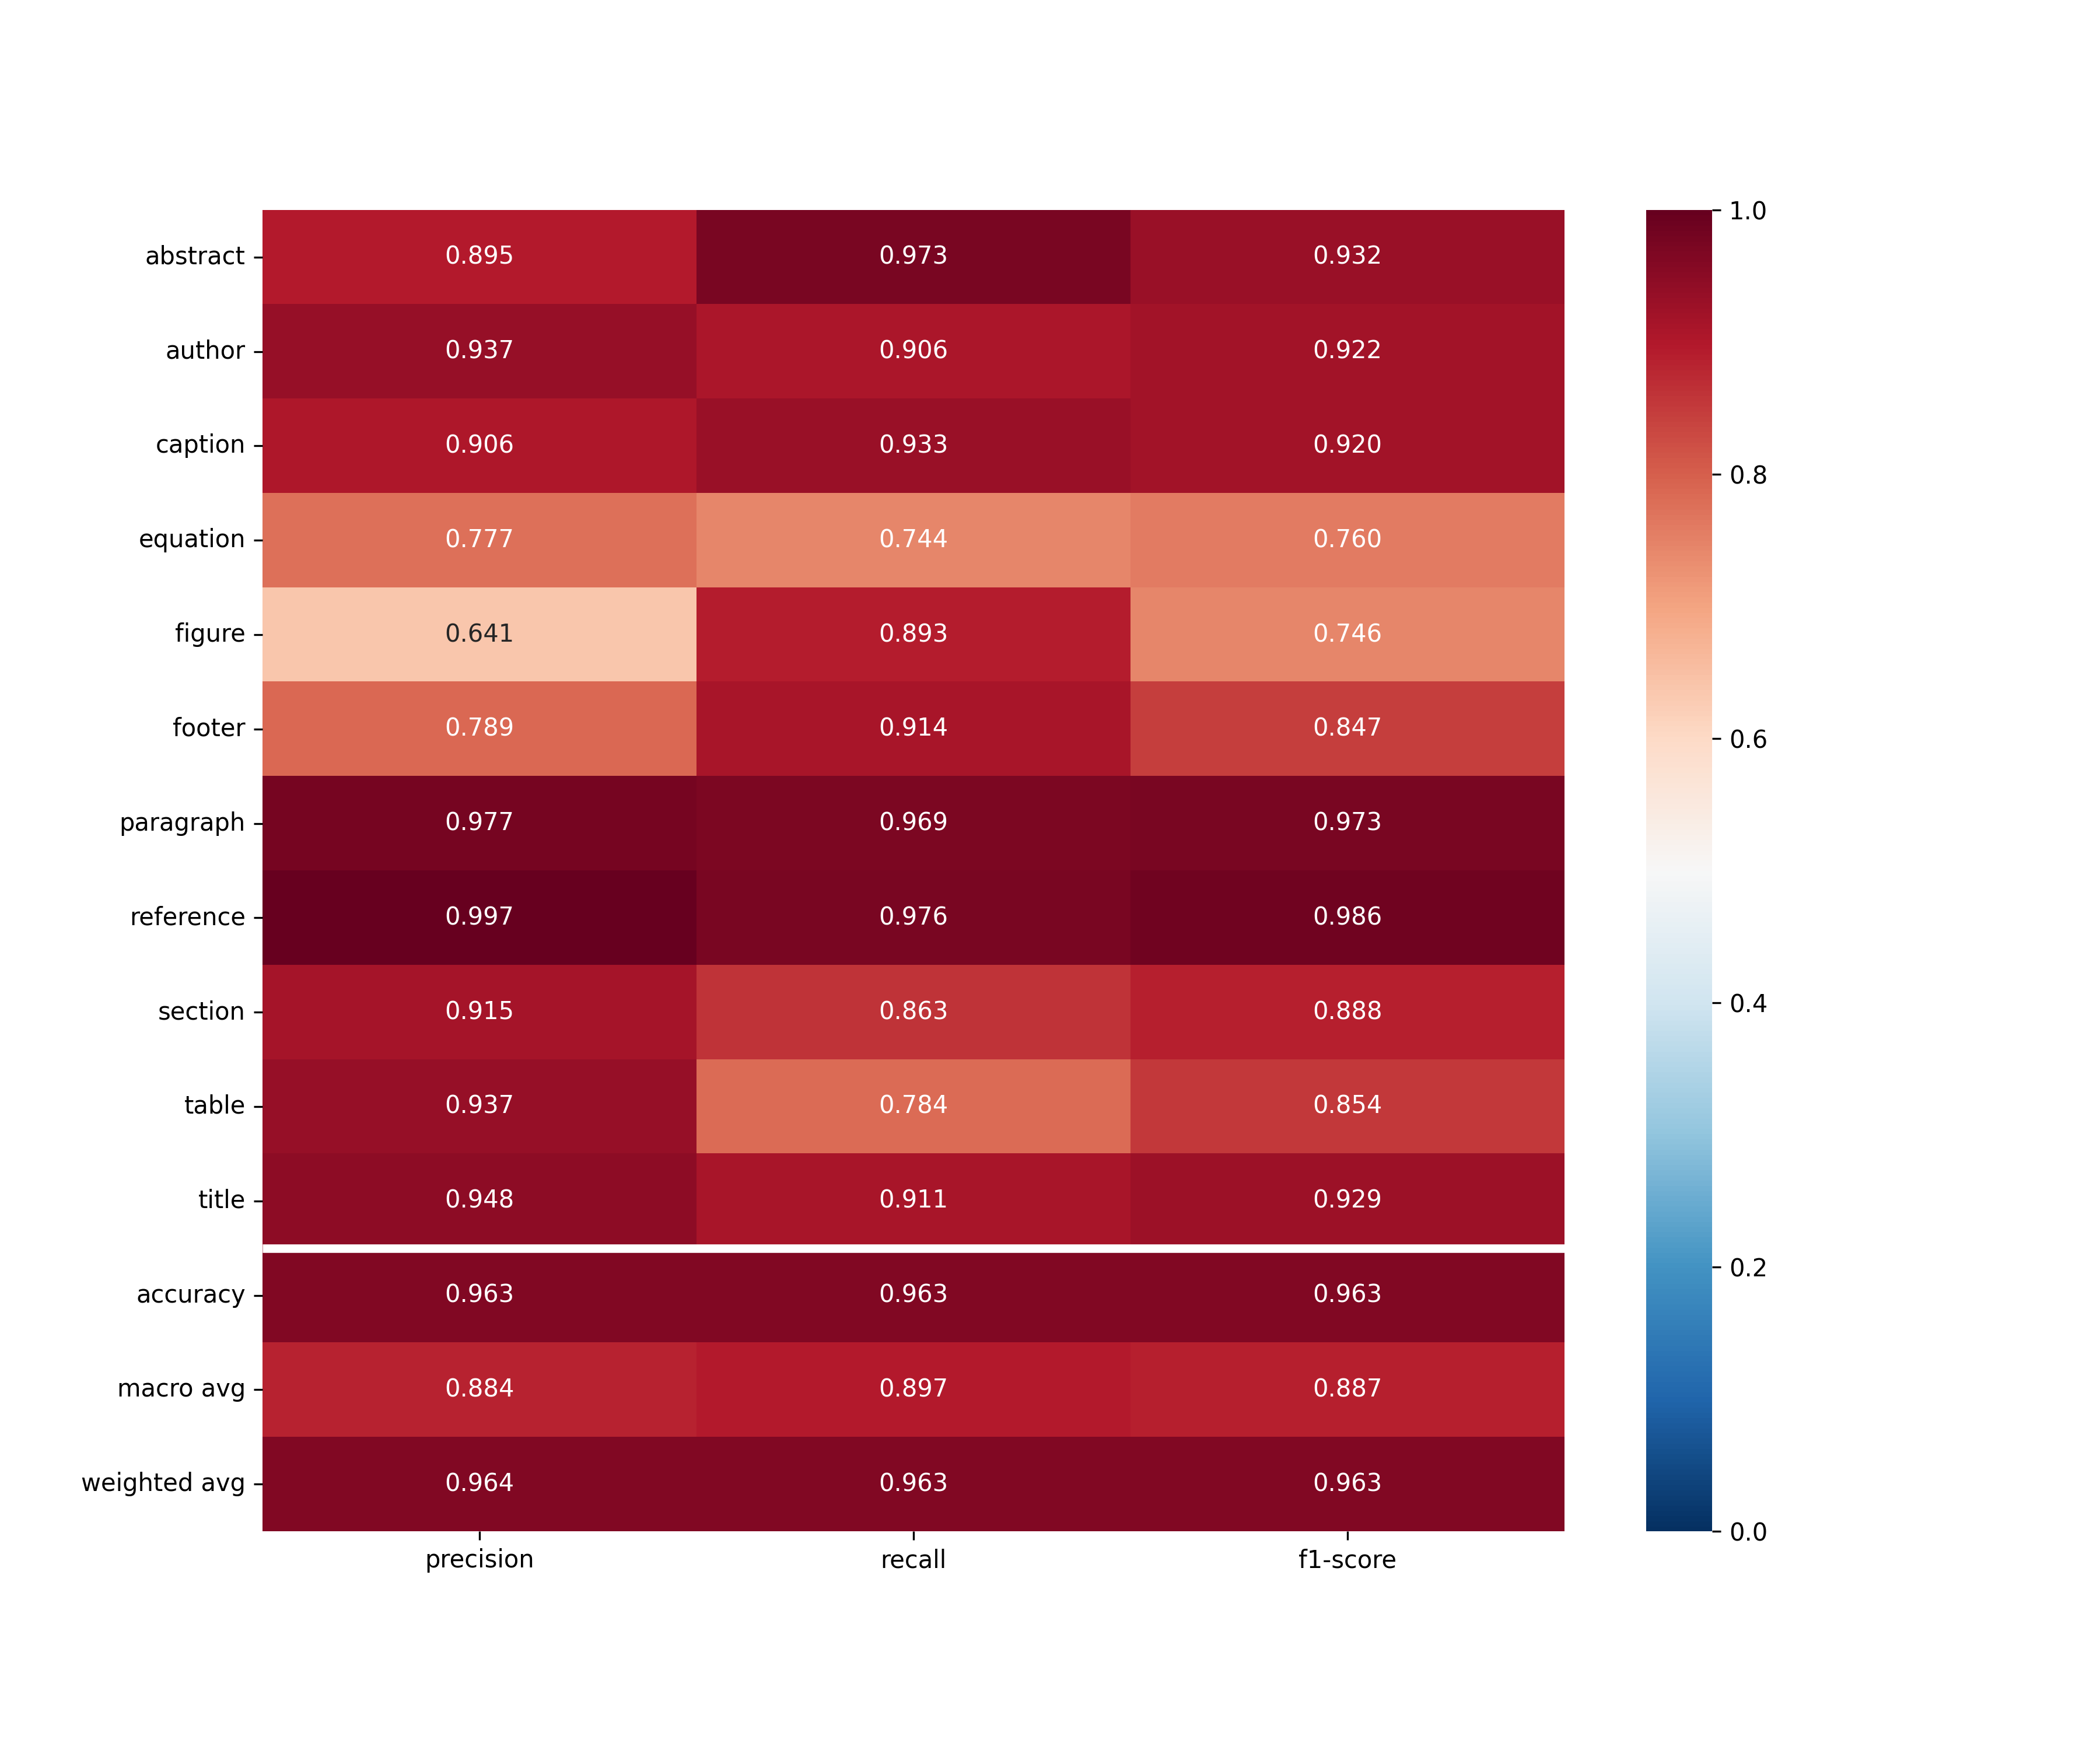
\includegraphics[trim=2cm 0 4cm 0, width=1.0\linewidth]{images/results/document_segmentation/docseg_cls_report_all.png}
    \caption{The resulting precision, recall, and F1-scores of our Document Segmentation Model utilized in BiBEx.}
    \label{fig:results_final_docseg_cls}
\end{figure}

\begin{figure}[bp!]
    \centering
    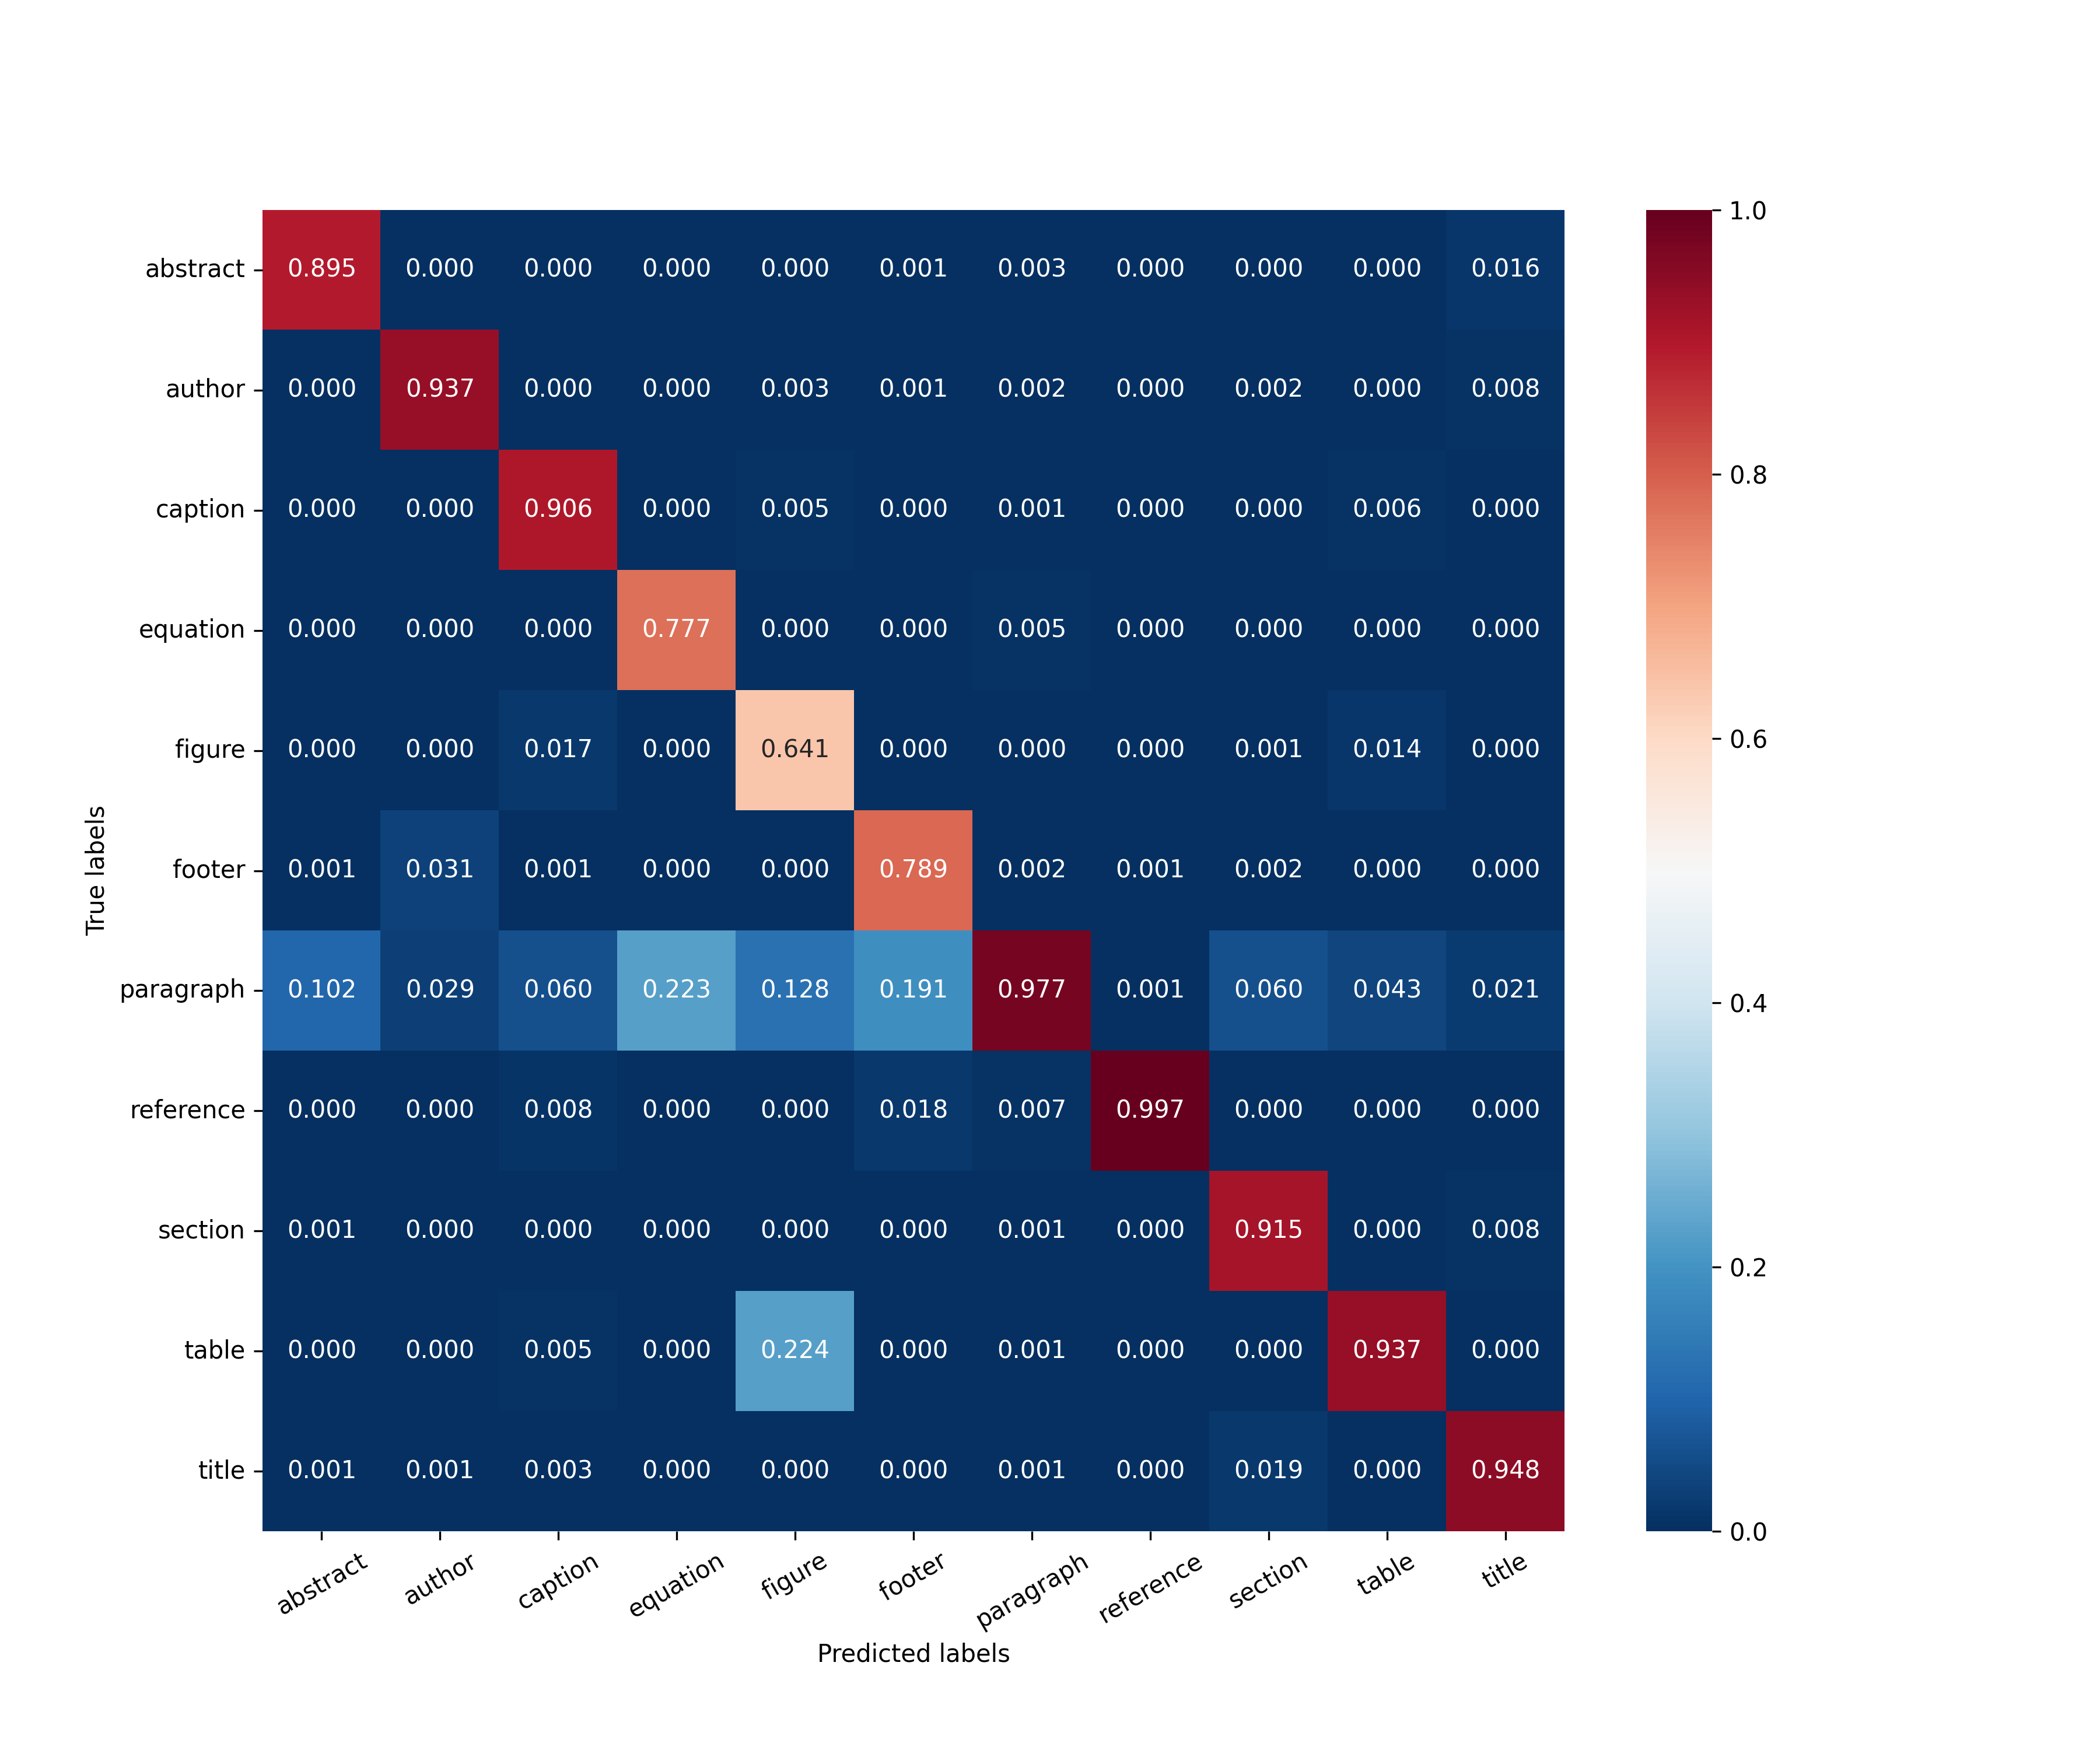
\includegraphics[trim=2cm 0 4cm 0, width=1.0\linewidth]{images/results/document_segmentation/docseg_conf_matrix_norm_pred_all.png}
    \caption{A confusion matrix, normalized over the predicted labels, of the Document Segmentation Model utilized in BiBEx.}
    \label{fig:results_final_docseg_conf}
\end{figure}
\FloatBarrier

\subsection{Reference Parser Model}\label{sec:eval_refseg}

Similar to our Document Segmentation Model in Section~\ref{sec:eval_docseg}, we optimized our hyperparameters using a grid search 5-fold crossvalidation. The hyperparameters that performed best were determined as follows: learning rate = 1e-5, batch size = 8, and epochs = 2. The $\alpha$ value to weight the loss function between the two outputs was set to $1.0$.\\
After optimizing the hyperparameters, we trained the Reference Parser Model using the entire training data and evaluated its performance by comparing its results against a mBERT~\cite{hug_cased_bert} and CRF model. The features utilized in the CRF model, were similar to those reported by Boukhers et al.~\cite{excite_methods} during the training of the EXparser system.\\
After analyzing the performance of our reference models, we implemented our custom classification head for the XLM-RoBERTa model. The results of both of the model's outputs, the label prediction and the new reference prediction, are depicted in Figures~\ref{fig:results_final_refseg_cls} and \ref{fig:results_final_refseg_ref}. A comparison of the entity prediction results of all models is visualized in Table~\ref{tab:results_refseg_compare}.

\begin{table}[!ht]
\centering
\begin{tabular}{l|
>{\columncolor[HTML]{DAE8FC}}l |
>{\columncolor[HTML]{EFEFEF}}l |
>{\columncolor[HTML]{DAE8FC}}l |}
\hline
\multicolumn{1}{|l|}{\textbf{label}}    & \textbf{CRF} & \textbf{mBERT} & \textbf{XLM-RoBERTa} \\ \hline\hline
\multicolumn{1}{|l|}{author}    & 0.743        & 0.877          & \textbf{0.891}       \\ \hline
\multicolumn{1}{|l|}{editor}    & 0.449        & 0.882          & \textbf{0.895}       \\ \hline
\multicolumn{1}{|l|}{fpage}     & 0.967        & 0.960          & \textbf{0.984}       \\ \hline
\multicolumn{1}{|l|}{issue}     & 0.706        & 0.715          & \textbf{0.847}       \\ \hline
\multicolumn{1}{|l|}{lpage}     & 0.980        & 0.974          & \textbf{0.983}       \\ \hline
\multicolumn{1}{|l|}{other}     & 0.695        & 0.758          & \textbf{0.795}       \\ \hline
\multicolumn{1}{|l|}{publisher} & 0.690        & 0.831          & \textbf{0.845}       \\ \hline
\multicolumn{1}{|l|}{source}    & 0.767        & 0.842          & \textbf{0.860}       \\ \hline
\multicolumn{1}{|l|}{title}     & 0.775        & \textbf{0.869} & 0.868                \\ \hline
\multicolumn{1}{|l|}{url}       & 0.753        & 0.500          & \textbf{0.907}       \\ \hline
\multicolumn{1}{|l|}{volume}    & 0.904        & 0.870          & \textbf{0.939}       \\ \hline
\multicolumn{1}{|l|}{year}      & 0.968        & 0.973          & \textbf{0.980}       \\ \hline\hline
\multicolumn{1}{|l|}{micro avg} & 0.816        & 0.876          & \textbf{0.907}       \\ \hline
\multicolumn{1}{|l|}{macro avg} & 0.783        & 0.838          & \textbf{0.899}       \\ \hline
\end{tabular}
\caption{A comparison of the entity prediction of our fine-tuned XLM-RoBERTa model and two reference models. Depicted are F1-scores.}
\label{tab:results_refseg_compare}
\end{table}

\begin{figure}[bp!]
    \centering
    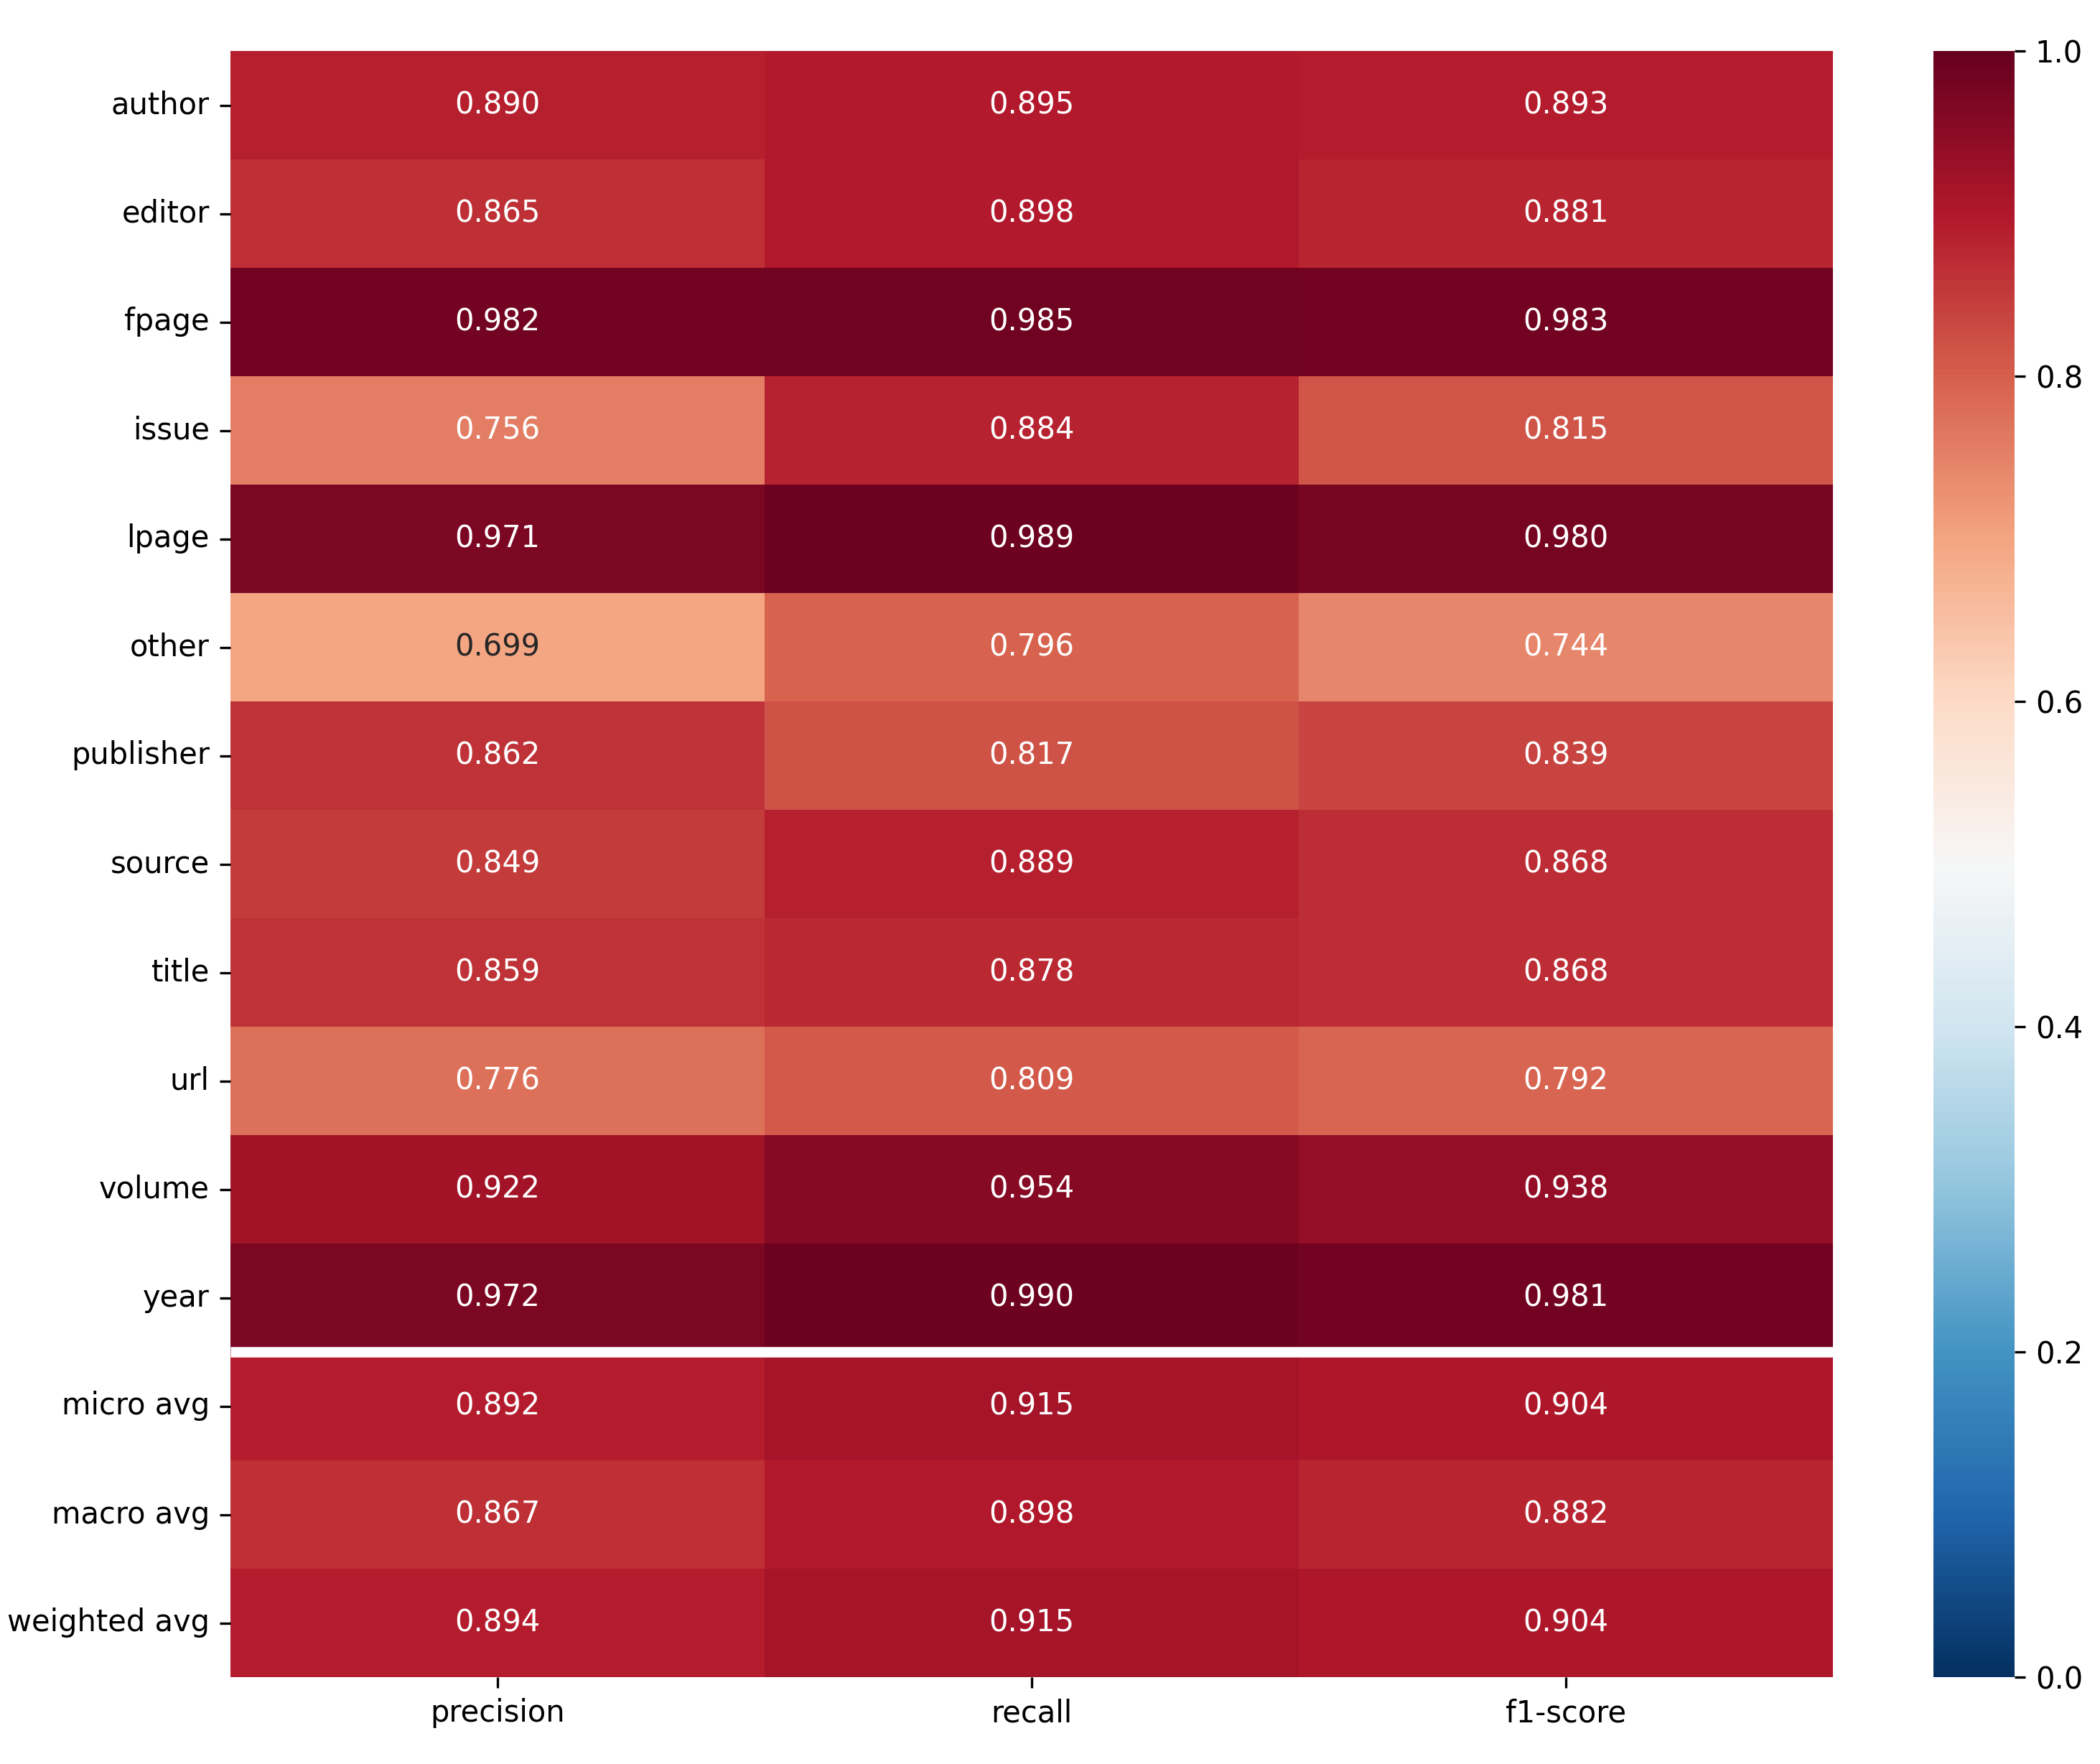
\includegraphics[width=1.0\linewidth]{images/results/reference_parser/ref_seg_cls_croped.png}
    \caption{The resulting precision, recall, and F1-scores of our Reference Parser Model utilized in BiBEx. Reported are the results of the entity prediction connected layer.}
    \label{fig:results_final_refseg_cls}
\end{figure}

\begin{figure}[bp!]
    \centering
    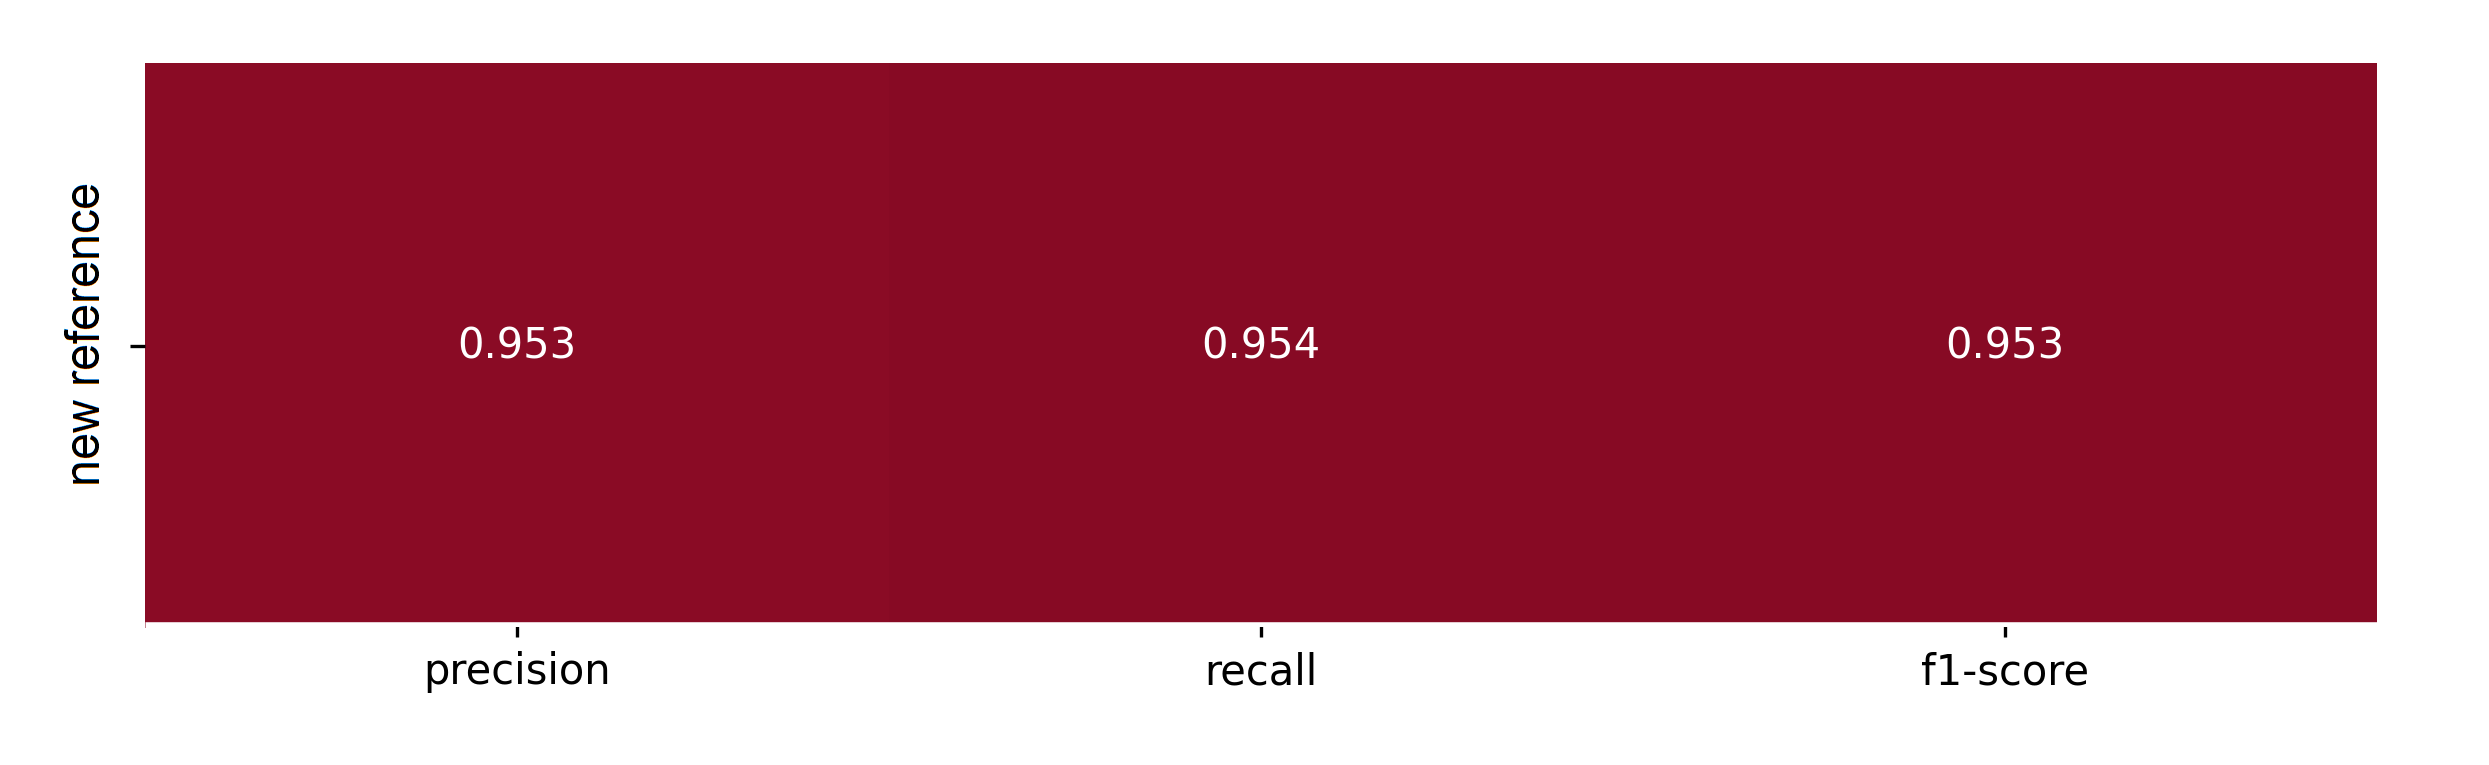
\includegraphics[width=0.8\linewidth]{images/results/reference_parser/ref_seg_croped.png}
    \caption{The resulting precision, recall, and F1-score of the connected layer, predicting a new reference of our Reference Parser Model utilized in BiBEx.}
    \label{fig:results_final_refseg_ref}
\end{figure}

\FloatBarrier

\subsection{Author Parser Model}
Equivalent to our our previous models in Section~\ref{sec:eval_docseg} and \ref{sec:eval_refseg}, we searched for the best hyperparameters utilizing a grid search with 5-fold crossvalidation. The selected hyperparameters are: learning rate = 5e-5, batch size = 16, and epochs = 2.\\
After optimizing our hyperparameters, we trained the Author Parser Model using our whole training set and evaluated its performance by comparing its results against a XLM-RoBERTa~\cite{hug_xlmr} and CRF model, as visualized in Table~\ref{tab:results_author_comp}. We further depict the performance of our final Author Parser Model in Figure~\ref{fig:results_author_cls} and visualize its results on various languages in Table~\ref{tab:results_author_lang}.

\begin{table}[!ht]
\centering
\begin{tabular}{l|
>{\columncolor[HTML]{DAE8FC}}l |
>{\columncolor[HTML]{EFEFEF}}l |
>{\columncolor[HTML]{DAE8FC}}l |}
%l|l|l|}
\hline
\multicolumn{1}{|l|}{\textbf{label}}                          & \textbf{CRF} & \textbf{mBERT} & \textbf{XLM-RoBERTa} \\ \hline\hline
\multicolumn{1}{|l|}{location}     & 0.777        & \textbf{0.905}          & 0.864                    \\ \hline
\multicolumn{1}{|l|}{organisation} & 0.701        & \textbf{0.823}          & 0.795                    \\ \hline
\multicolumn{1}{|l|}{person}       & 0.849        & \textbf{0.919}          & 0.909                    \\ \hline\hline
\multicolumn{1}{|l|}{micro avg}    & 0.816        & \textbf{0.882}          & 0.858                    \\ \hline
\multicolumn{1}{|l|}{macro avg}    & 0.783        & \textbf{0.869}          & 0.856                    \\ \hline
\end{tabular}
\caption{The resulting F1-scores of the Author Parser Model compared with a CRF and XLM-RoBERTa model.}
\label{tab:results_author_comp}
\end{table}

\begin{table}[!ht]
\centering
\begin{tabular}{|c|
>{\columncolor[HTML]{DAE8FC}}l |
>{\columncolor[HTML]{EFEFEF}}l |
>{\columncolor[HTML]{DAE8FC}}l |}
\hline
\multicolumn{1}{|l|}{\textbf{language}} & \textbf{location} & \textbf{organisation} & \textbf{person} \\ \hline\hline
German                                  & 0.899             & 0.809                                      & 0.912           \\ \hline
English                                 & 0.876             & 0.766                                      & 0.888           \\ \hline
French                                  & 0.921             & 0.849                                      & 0.940           \\ \hline
Spanish                                 & 0.922             & 0.870                                      & 0.937           \\ \hline
\end{tabular}
\caption{The resulting F1-scores by language of the Author Parser Model utilized by BiBEx.}
\label{tab:results_author_lang}
\end{table}

\begin{figure}[bp!]
    \centering
    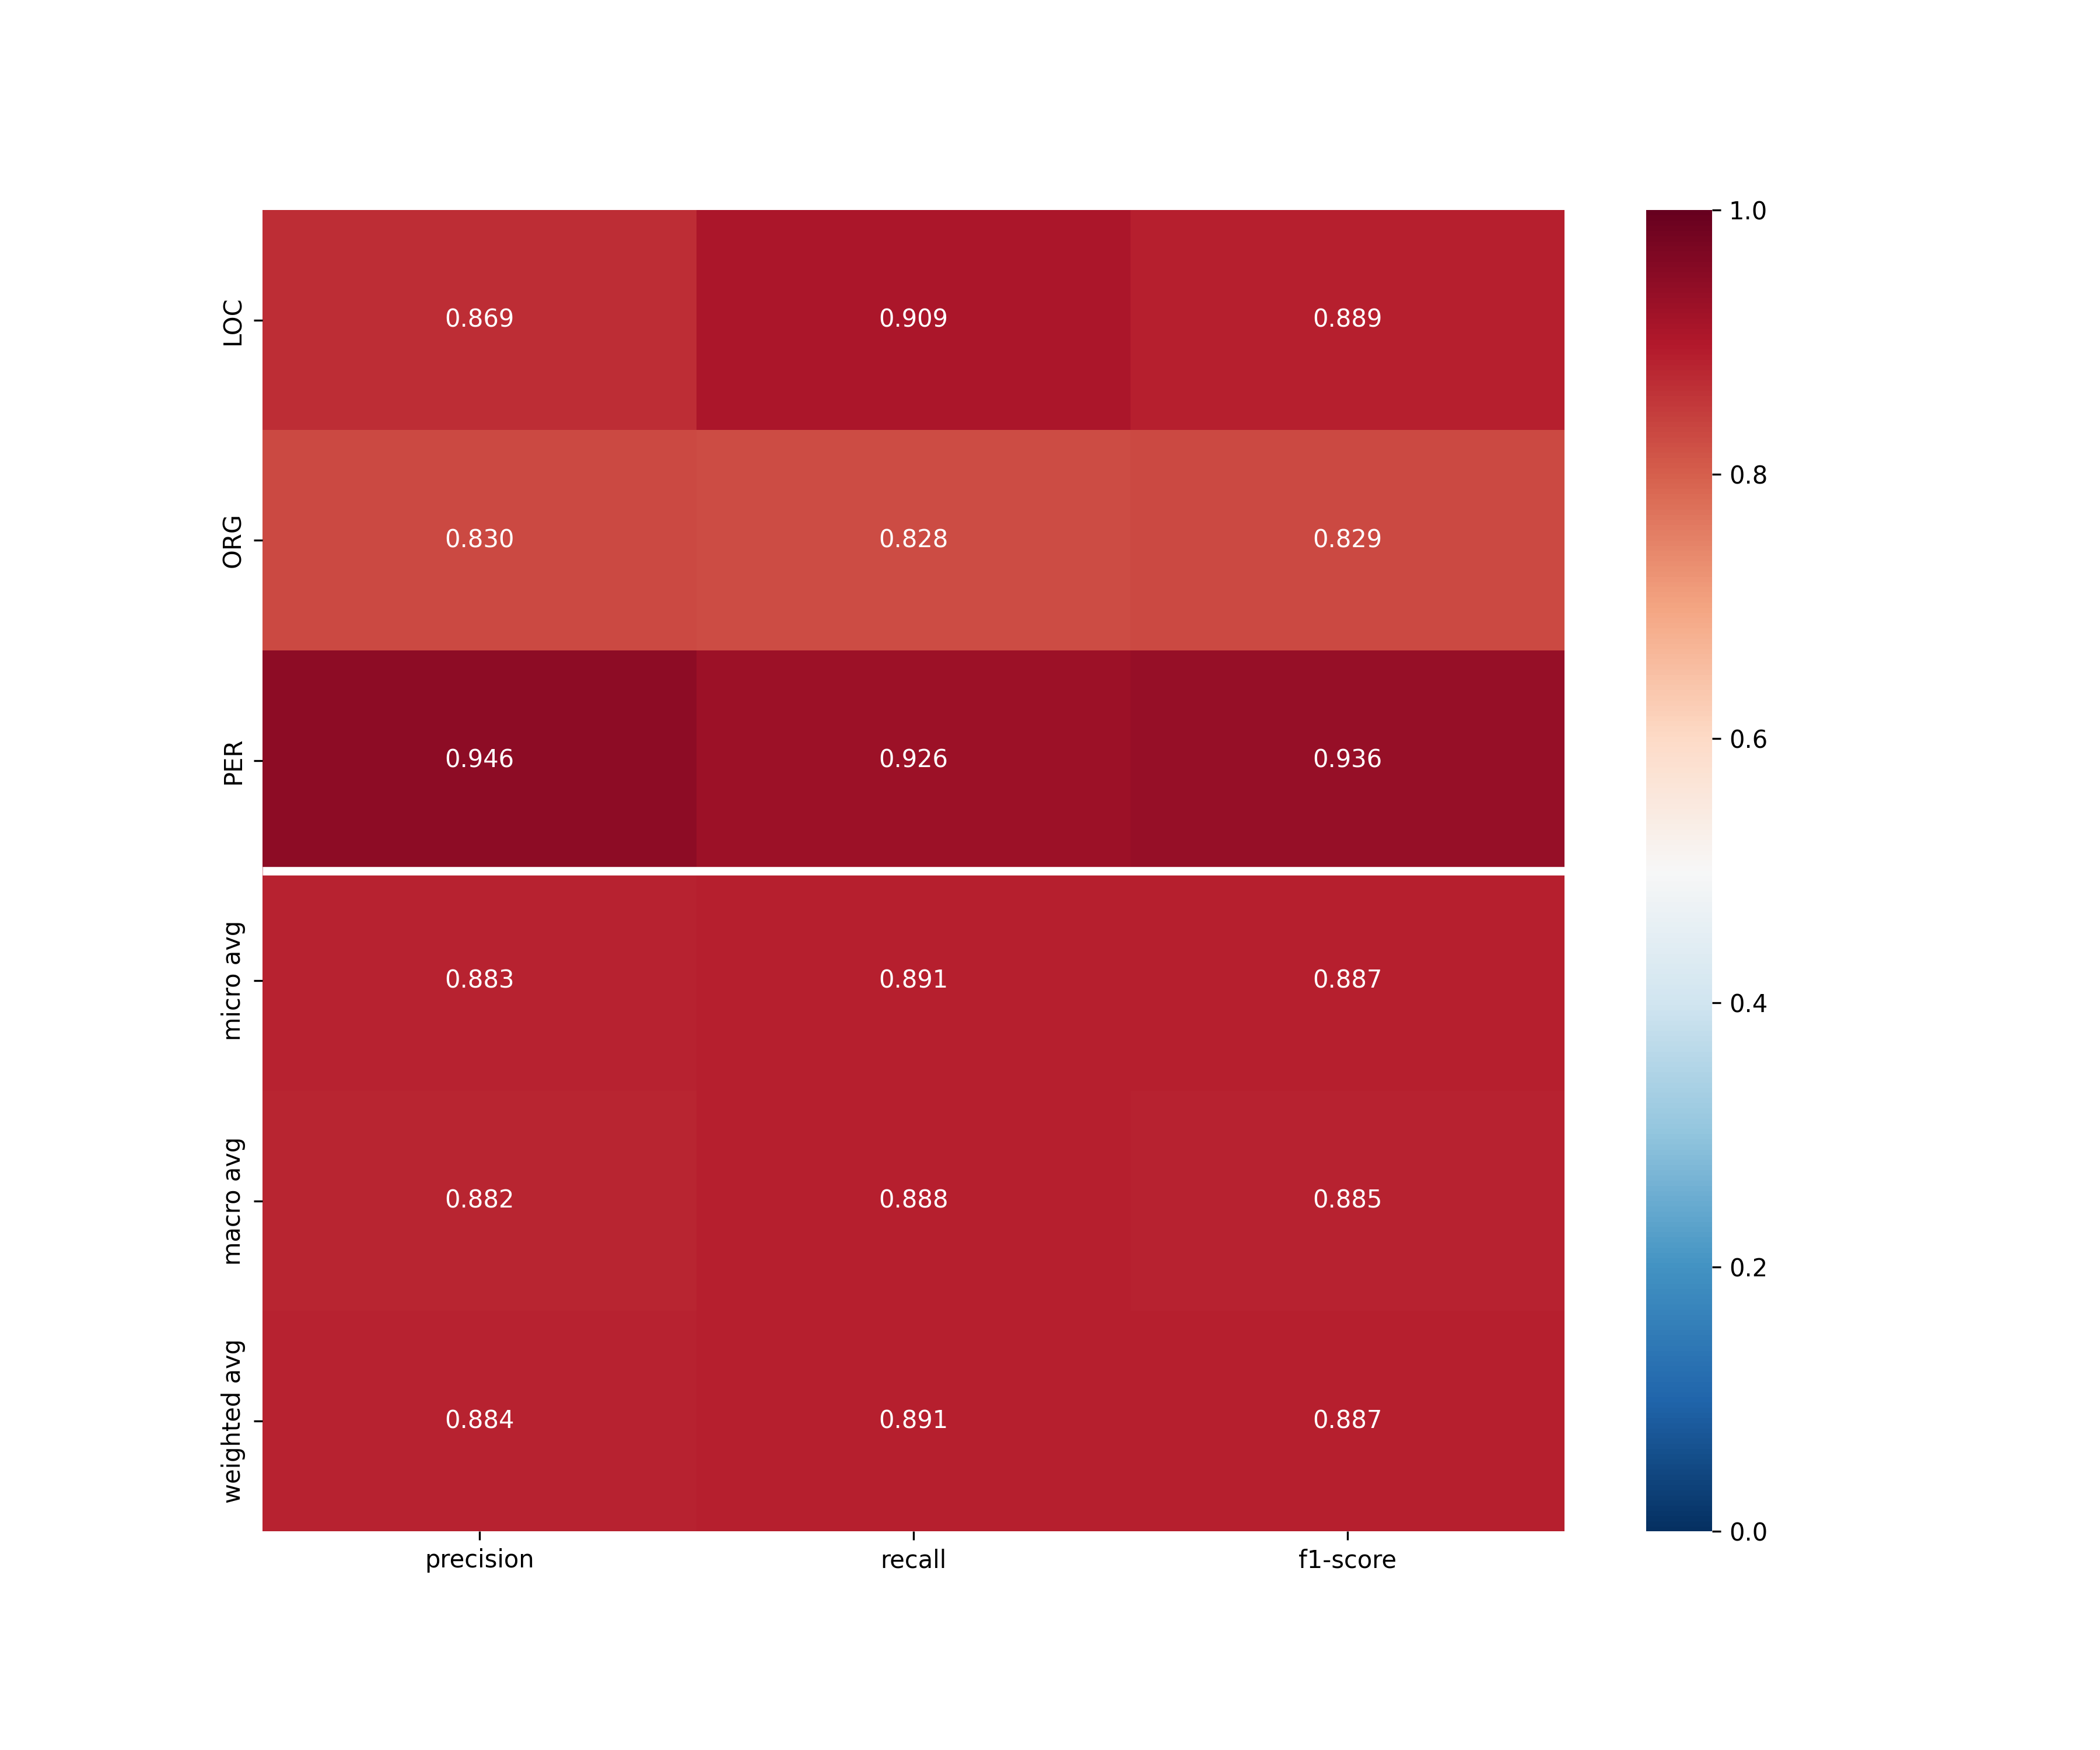
\includegraphics[trim=2cm 0 4cm 0, width=1.0\linewidth]{images/results/author_parser/ner_bert_de_cls_report.png}
    \caption{The resulting precision, recall, and F1-scores of our Author Parser Model used in BiBEx.}
    \label{fig:results_author_cls}
\end{figure}

\FloatBarrier

\section{Extrinsic Evaluation}\label{sec:results_extrinsic}
In this section, we will explain the methods and strategies we employed to evaluate the performance of our overall system. We will discuss the challenges we encountered and the solutions we devised. Our general aim is to assess how effectively our various models and techniques work together.\\
Evaluating the entire system poses a challenge as it requires both visual information, such as images or PDFs, and structured metadata to compare our predictions against. Additionally, to conduct an evaluation of our system, we need metadata containing the authors of an article, as well as segmented and parsed reference entities.\\
However, datasets that fulfill all of these requirements are rare. To address this, we decided to evaluate our system using two distinct datasets. One dataset was used to assess the quality of author extraction, while the other was utilized to evaluate the reference extraction process.

\subsection{Author Extraction}
For the document author evaluation, we curated a corpus by gathering literature from the Social Science Open Access Repository~\cite{noauthor_ssoar_nodate}. The SSOAR provides full-text literature as PDF files, specifically scholarly publications from the domain of social sciences, as well as corresponding metadata.\\
To assemble our corpus, we specifically queried for open access documents related to the field of Geography, ensuring that the file sizes were below 10 MByte to accommodate bandwidth and computational constraints. We processed articles with no more than 30 pages and disregarded those documents, which caused errors during the extraction. This yielded a diverse collection of 2,032 historical and modern-day documents from 2,501 authors, consisting of scientific articles written in various languages, with German and English being the predominant ones. These documents served as the foundation for evaluating the performance of our document author extraction.\\
In our evaluation, we compared our models against the GROBID BiLSTM-CRF and CRF backend as reference models. During the analysis of our corpus, we observed instances where the authors extracted from metadata files did not perfectly align with the corresponding text in the OCR layers. This discrepancy was most likely caused by errors during the OCR process of these articles, like mix-ups between lowercase \enquote{i} and lowercase \enquote{l}.\\
To address this issue and improve the matching criteria, we adopted a two-fold approach. Firstly, we utilized an exact matching criterion where each character of the predicted author and the true author had to coincide for a strict comparison.\\
Secondly, we incorporated the Levenshtein distance~\cite{levenshtein1966binary}, which allowed for a more relaxed matching criteria, enabling us to handle cases with slight differences between the extracted and true authors. The results are shown in Table~\ref{tab:results_overall_author}.

\begin{table}[!ht]
\centering
\begin{tabular}{l|ll|ll|ll|}
\cline{2-7}
                                & \multicolumn{2}{c|}{\textbf{BiBEx}}                                                & \multicolumn{2}{c|}{\textbf{GROBID$^{DL}$}}                                    & \multicolumn{2}{c|}{\textbf{GROBID$^{CRF}$}}                                           \\ \cline{2-7} 
\textbf{}                       & \multicolumn{1}{l|}{exact}                   & loose                   & \multicolumn{1}{l|}{exact}                   & loose                   & \multicolumn{1}{l|}{exact}                   & loose                   \\ \hline
\multicolumn{1}{|l|}{precision} & \multicolumn{1}{l|}{\cellcolor[HTML]{DAE8FC}0.716} & \cellcolor[HTML]{EFEFEF}0.747 & \multicolumn{1}{l|}{\cellcolor[HTML]{DAE8FC}0.377} & \cellcolor[HTML]{EFEFEF}0.389 & \multicolumn{1}{l|}{\cellcolor[HTML]{DAE8FC}0.511} & \cellcolor[HTML]{EFEFEF}0.528 \\ \hline
\multicolumn{1}{|l|}{recall}    & \multicolumn{1}{l|}{\cellcolor[HTML]{DAE8FC}0.703} & \cellcolor[HTML]{EFEFEF}0.734 & \multicolumn{1}{l|}{\cellcolor[HTML]{DAE8FC}0.526} & \cellcolor[HTML]{EFEFEF}0.543 & \multicolumn{1}{l|}{\cellcolor[HTML]{DAE8FC}0.511} & \cellcolor[HTML]{EFEFEF}0.529 \\ \hline
\multicolumn{1}{|l|}{F1-score}  & \multicolumn{1}{l|}{\cellcolor[HTML]{DAE8FC}0.710} & \cellcolor[HTML]{EFEFEF}0.741  & \multicolumn{1}{l|}{\cellcolor[HTML]{DAE8FC}0.439} & \cellcolor[HTML]{EFEFEF}0.453 & \multicolumn{1}{l|}{\cellcolor[HTML]{DAE8FC}0.511} & \cellcolor[HTML]{EFEFEF}0.529 \\ \hline
\end{tabular}
\caption{The resulting precision, recall, and F1-scores of the article author extraction process. We compare BiBEx and GROBID with the BiLSTM-CRF (DL) and CRF backend. The loose matching utilizes a Levenshtein distance of 1, for matching predicted and true authors.}
\label{tab:results_overall_author}
\end{table}

\subsection{Reference Extraction}
To evaluate the quality of our citation metadata extraction process, we utilized the dataset provided by Cioffi et al.~\cite{cioffi2022structured} as a gold standard. This dataset consists of 56 documents, comprising 2,538 reference strings, and encompasses articles from various domains. The authors of this dataset offer open-access articles in the form of PDF files, along with corresponding bibliographic metadata. The dataset is designed as a benchmark for assessing the efficacy of metadata extraction tools of scientific publications.
In their evaluation, the authors propose a 3-fold evaluation methodology, which distinguishes between three metrics:
\newpage

\begin{itemize}
    \item The first evaluation metric focuses on correctly identified references, assessing a tool's capability to distinguish each reference from the surrounding text and other references.
    \item The second evaluation aspect measures the number of correctly tagged metadata entities per reference, irrespective of the correctness of the content itself.
    \item The third evaluation feature measures the number of correctly parsed and tagged contents within each bibliographic reference.
\end{itemize}

After extracting bibliographic references from this dataset, we transformed our outputs from a JSON format to a TEI format to enable a comparison with other systems. Our evaluation involved comparing our results against those obtained from GROBID, CERMINE, ParsCit, and Anystyle, which was found to yield the best overall performance in the evaluation conducted by Cioffi et al. The results are visualized in Table~\ref{tab:results_reference_extraction}.

\begin{table}[!ht]
\begin{tabular}{cl|
>{\columncolor[HTML]{DAE8FC}}l |
>{\columncolor[HTML]{EFEFEF}}l |
>{\columncolor[HTML]{DAE8FC}}l |
>{\columncolor[HTML]{EFEFEF}}l |
>{\columncolor[HTML]{DAE8FC}}l |}
%l|l|l|l|l|}
% >{\columncolor[HTML]{EFEFEF}}l |l|
% >{\columncolor[HTML]{EFEFEF}}l |l|
% >{\columncolor[HTML]{EFEFEF}}l |}
\cline{3-7}
\multicolumn{1}{l}{}                                        & \textbf{} & \textbf{CERMINE} & \textbf{GROBID}        & \textbf{EXCITE} & \textbf{Anystyle}      & \textbf{BiBEx}         \\ \hline
\multicolumn{1}{|c|}{}                                      & precision & 0.75    & 0.54          & 0.59   & 0.81          & \textbf{0.83} \\ \cline{2-7} 
\multicolumn{1}{|c|}{}                                      & recall    & 0.67    & 0.55          & 0.53   & 0.74          & \textbf{0.86} \\ \cline{2-7} 
\multicolumn{1}{|c|}{\multirow{-3}{*}{\textbf{references}}} & F1-score  & 0.71    & 0.54          & 0.56   & 0.77          & \textbf{0.84} \\ \hline\hline
\multicolumn{1}{|c|}{}                                      & precision & 0.94    & 0.86          & 0.93   & 0.93          & \textbf{0.95} \\ \cline{2-7} 
\multicolumn{1}{|c|}{}                                      & recall    & 0.94    & \textbf{0.97} & 0.93   & \textbf{0.97} & \textbf{0.97} \\ \cline{2-7} 
\multicolumn{1}{|c|}{\multirow{-3}{*}{\textbf{metadata}}}   & F1-score  & 0.94    & 0.91          & 0.93   & 0.95          & \textbf{0.96} \\ \hline\hline
\multicolumn{1}{|c|}{}                                      & precision & 0.86    & 0.81          & 0.8    & 0.87          & \textbf{0.88} \\ \cline{2-7} 
\multicolumn{1}{|c|}{}                                      & recall    & 0.87    & \textbf{0.91} & 0.8    & \textbf{0.91} & 0.9           \\ \cline{2-7} 
\multicolumn{1}{|c|}{\multirow{-3}{*}{\textbf{content}}}    & F1-score  & 0.86    & 0.86          & 0.8    & \textbf{0.89} & \textbf{0.89} \\ \hline\hline
\end{tabular}
\caption{The resulting precision, recall, and F1 scores of the BiBEx reference extraction process compared to various other extraction tools.}
\label{tab:results_reference_extraction}
\end{table}
\chapter{Discussion}\label{chap:discussion}
In this chapter, we will discuss the results obtained from our intrinsic (Section~\ref{sec:discussion_intrinsic}) and extrinsic (Section~\ref{sec:discussion_extrinsic}) evaluations. We will discuss the performance of our models and the overall system. Additionally, we aim to address the limitations and challenges encountered during the evaluation process (Section~\ref{sec:discussion_limitations}).\\
We will assess whether the models we employed and the overall BiBEx system can effectively address our research questions. We aim to determine if the system we developed is robust and unified, capable of accurately extracting metadata from document headers and references, irrespective of the language in which they are written, be it English or German.

\section{Intrinsic Evaluation}\label{sec:discussion_intrinsic}
% document segmentation
As evident in Table~\ref{tab:results_document_segment_compare}, our experiments show that our fine-tuned LayoutXLM model achieved the best results in almost all categories, except in the figure class. This may seem counterintuitive, since the LayoutXLM architecture explicitly envelops visual information and figures should be one of the most striking features in a document.\\
We believe that this is the result of the different creation processes of our self-annotated dataset and the DocBank dataset. Figures in the DocBank dataset are assigned the token '\textit{\#\#LTFigure\#\#}' and '\textit{\#\#LTLine\#\#}' with bounding boxes enclosing the entire figure. As we can see in Table~\ref{tab:results_docseg_lang}, the LayoutXLM model is capable to nearly perfectly predict figure labels of the DocBank portion of the dataset.\\
OCR systems on the other hand usually do not extract illustrations as a whole and instead try to distil text from these images. This can result in artefacts, where the OCR system detects non-existing text or text fragments in figures. Due to our premise to create a robust dataset, we decided to keep these artefacts and label them as figures. We believe that these artefacts can stand out in a coherent text, which is why text-based classifiers can accurately predict them.\par
We observed also fairly high F1-scores for the '\textit{reference}' class of all employed models with only the CRF model performing worse than the rest. However, our results suggest that visual information might not be the predominant feature to detect reference sections in articles, since both mBERT and XLM-RoBERTa show good results, relying only on textual information.\\
On the other hand show classes we are predominately interested in, namely author, abstract, and title considerable improvements against their reference models. These classes typically protrude in articles, for example are title often written in a bigger font or abstracts highlighted in bold. This suggests, that the visual information fed into LayoutXLM indeed seems to facilitate the models ability to correctly predict its classes.\\

\begin{figure}[!ht]
    \centering
    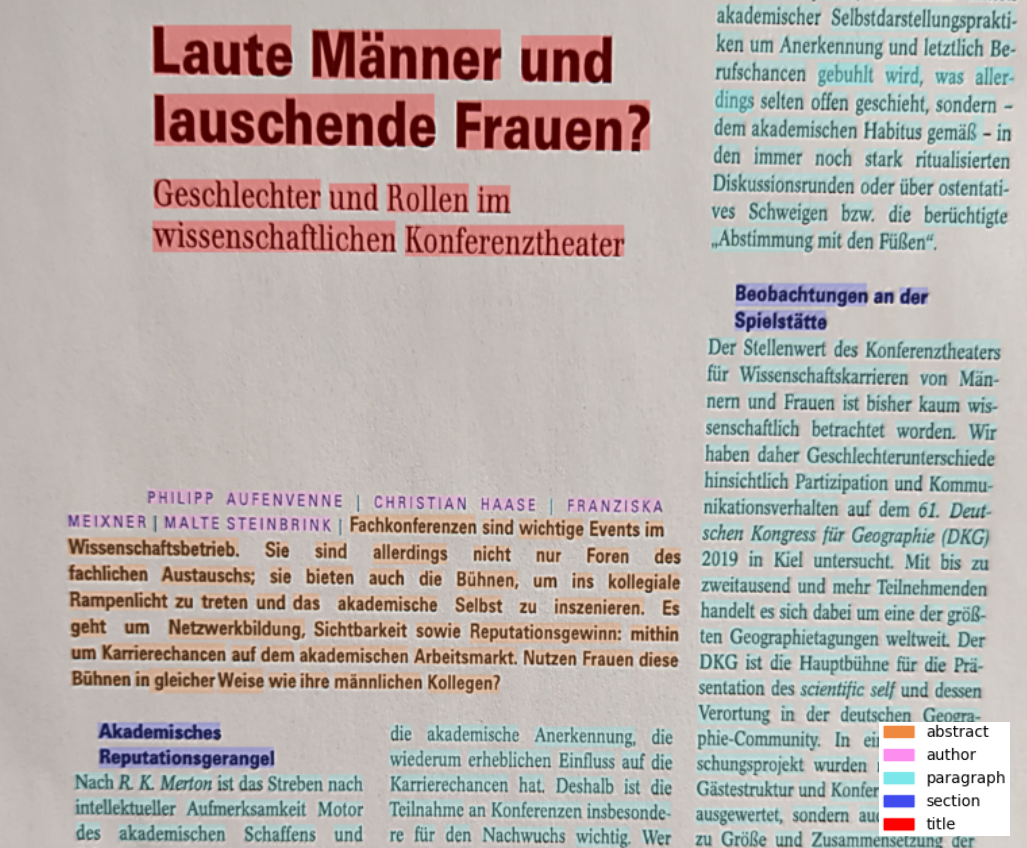
\includegraphics[width=0.85\linewidth]{images/layoutxlm.png}
    \caption{The detected classes of an article by our fine-tuned LayoutXLM model. Despite the faulty layout caused by the OCR process, as depicted in Figure~\ref{fig:layout_error}, we are able to extract all authors.}
    \label{fig:layoutxlm_result}
\end{figure}

The confusion matrix depicted in Figure~\ref{fig:results_final_docseg_conf} shows a slight bias for some labels towards the majority class '\textit{paragraph}'. In many cases these errors occurred in articles, where text segments of a certain class are unusually long, for example long abstracts or footer sections. LayoutXLM is further constricted by the amount of maximum token it can predict, which can remove contextual information surrounding long sections. All of this hinders the correct classification of long text sections for certain classes.\\
Furthermore, we noticed that documents with less discriminating visual features, as shown for example in Figure~\ref{fig:no_seperation}, where we have no clear separation between abstract and the following text section, are prone to have higher error rates.\\
\begin{figure}[!t]
    \centering
    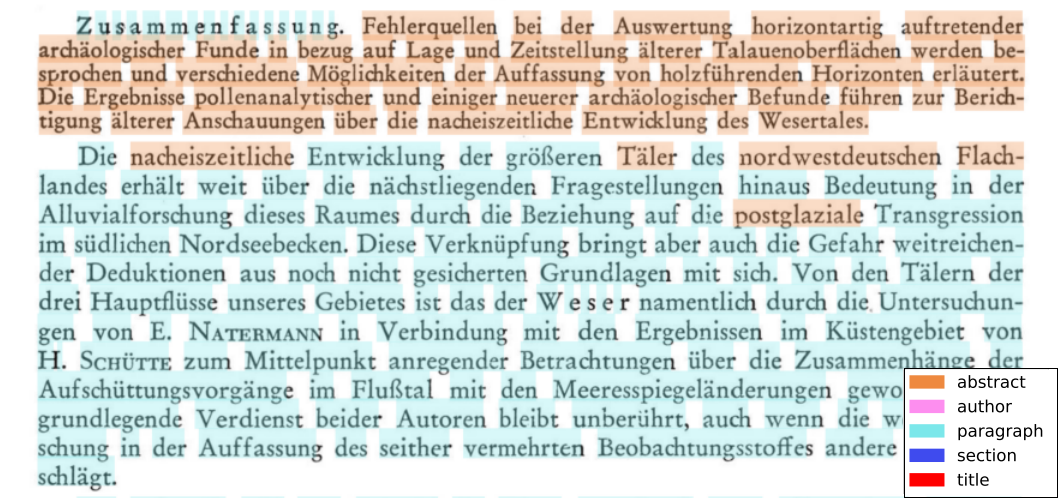
\includegraphics[width=0.8\linewidth]{images/no_seperation.png}
    \caption{An article with a less salient layout. Our model has a hard time predicting the end of the abstract section.}
    \label{fig:no_seperation}
\end{figure}
We also noticed better results on the DocBank portion of our created Document Segmentation dataset, as evident in Table~\ref{tab:results_docseg_lang}. We mainly attribute this to the overall homogeneity of the articles comprising the DocBank dataset, as these modern documents are created through the \LaTeX~typesetting system and mostly employ "streamlined" layouts and structure.\\
On the other hand, we have historic articles, which are far more diverse regarding structure and layout, for example articles beginning with an abstract followed by author and title, complicating the segmentation process.\\
References were even better detected by our model in the GEOcite portion of the dataset, suggesting that the internal text structure of reference strings might contribute more towards identification of references than visual information.\par
% reference parser
For the Reference Parser Model, we can also see a clear improvement of both transformer models against the CRF baseline model, as depicted in Table~\ref{tab:results_refseg_compare}. XLM-RoBERTa outperformed the fine-tuned mBERT model by a slight margin.\\
However, we encountered challenges while replicating the reported results for CRF models as documented by Boukhers et al.~\cite{excite_methods}. This discrepancy may indicate that the CRF model struggles with long-term dependencies in our reference segments, given that our dataset comprises reference segments instead of individual reference strings.\\
Despite facing a minor decrease in overall results following the implementation of our custom classification header and fine-tuning our model, both outputs still demonstrate favorable performance, as indicated in Figures~\ref{fig:results_final_refseg_cls} and~\ref{fig:results_final_refseg_ref}.\\
We further observed a difficulty in correctly classifying long URLs using our Reference Parser Model. Despite the expectation that the model would perform well on this class due to the fixed structure of URLs, we encountered challenges. We attribute this issue to the preprocessing of several special characters, which leads to the tokenization of URL sequences into long input sequences for our model. As a result, predicting them as a whole coherent class becomes challenging as showcased in Figure~\ref{fig:url_error}.

\begin{figure}[!t]
    \centering
    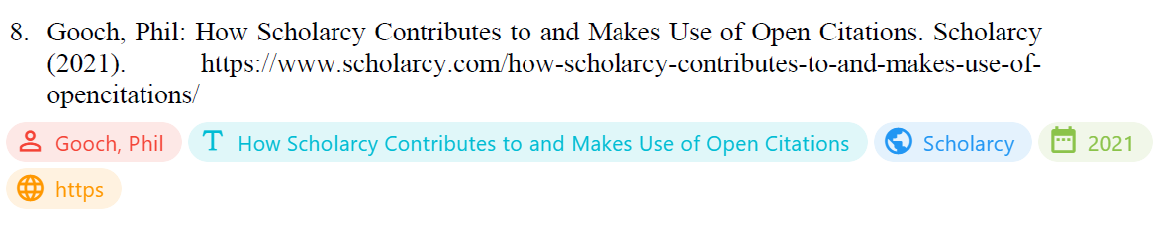
\includegraphics[width=1.0\linewidth]{images/url.png}
    \caption{An exemplary citation, where BiBEx was not able to extract the URL.}
    \label{fig:url_error}
\end{figure}

% author parser
The Author Parser Model showed similar results as the Document Segmentation Model and Reference Parser Model, where the CRF baseline model was outperformed by both transformer models, as indicated in Table~\ref{tab:results_author_comp}.\\
In our experiments, we used a cased version of XLM-RoBERTa since an uncased version, pretrained on a suitable corpus was not available at the time. Despite the expectation that the cased model might perform better, considering that upper case letters are strong indicators of a person's name, the fine-tuned mBERT model displayed better results than the XLM-RoBERTa model.\\
In general, we observed good results for all languages in our test set, with slightly lower performance for the English corpus compared to other languages, as shown in Table~\ref{tab:results_author_lang}.

\section{Extrinsic Evaluation}\label{sec:discussion_extrinsic}
As shown in Table~\ref{tab:results_overall_author}, the BiLSTM-CRF backend of GROBID performs worse than the CRF backend on our test corpus. This discrepancy might be due to various reasons such as differences in training data or an altered tokenization process. Further investigation and experimentation would be needed to determine the exact cause of this difference.\\
We observed that GROBID tends to extract tokens surrounding the title, leading to misclassifications such as labeling parts of the affiliation as authors. Additionally, it encounters difficulties when an article starts not directly at the top of a document page, especially if another article is present on the same page. These challenges may affect the overall performance of GROBID in our context, since the GEOcite corpus consists of various journals, where the end of an article and the start of another essay can be located on the same page.\\
In the case of BiBEx, we observed that the application often extracted correct author names, but faced challenges in accurately matching the actual author due to the limitations of our heuristics. These limitations can lead to wrongly split names, particularly in cases where the surname consists of multiple words, such as the nobiliary particles \enquote{af}, \enquote{von}, and \enquote{de}.\\
\begin{figure}[!ht]
    \centering
    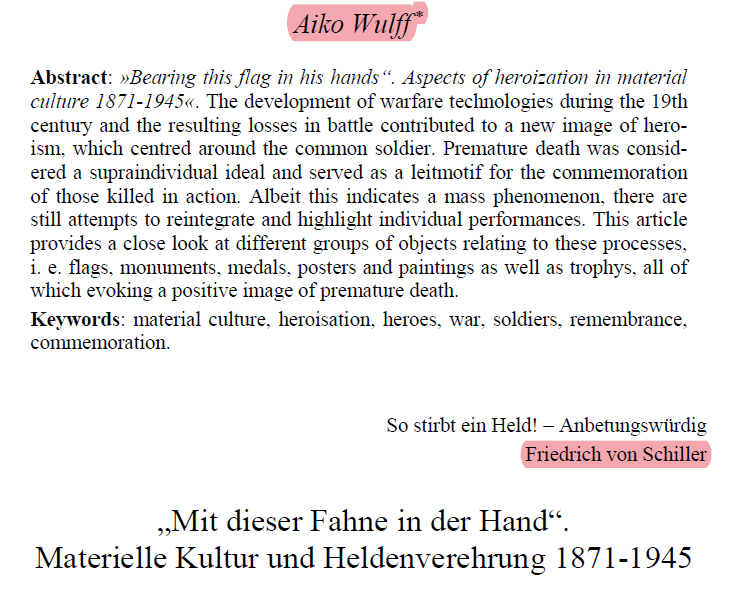
\includegraphics[width=0.6\linewidth]{images/bibex_author_wrong.png}
    \caption{BiBEx correctly predicts \enquote{Aiko Wulff}, but wrongly classifies \enquote{Friedrich von Schiller} as one of the authors of this article.}
    \label{fig:author_error}
\end{figure}
Furthermore, BiBEx occasionally misclassifies a person's name as an author, especially when they are in close proximity to the title. For instance, this can occur when an article is dedicated to a specific person, mentions editors, or displays a quote near the title, as seen in Figure~\ref{fig:author_error}.\\
During the reference extraction, as discussed in Section~\ref{sec:discussion_intrinsic}, BiBEx faces challenges when identifying URLs. Additionally, we observed that entities with long hyphenated sequences, such as titles, can occasionally be split into two or more entities of the same class.\\
On the positive side, our proposed system demonstrates effectiveness in distinguishing header sections of articles from citations, as illustrated in Figure~\ref{fig:ref_header}. This distinction is crucial, as it prevents falsely identified self-citations, a common occurrence with other tools.\\
As indicated in Table~\ref{tab:results_overall_author}, the BiBEx extraction application outperforms or achieves comparable results in most metrics for reference extraction. This is a promising outcome, indicating the effectiveness and robustness of our reference extraction approach.

\begin{figure}[!t]
    \centering
    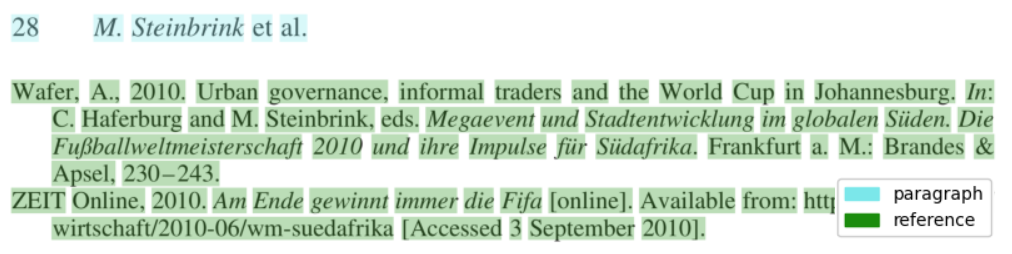
\includegraphics[width=0.9\linewidth]{images/header.png}
    \caption{BiBEx correctly classifies the header section of a page as paragraph, which could lead to false self-citations in a citation network, in case of a failure.}
    \label{fig:ref_header}
\end{figure}

\section{Limitations}\label{sec:discussion_limitations}

As described in our conceptual framework (Section~\ref{sec:conceptual_framework}), we intentionally limited the complexity of our BiBEx system to reduce potential errors stemming from upstream models. However, our findings indicate that the heuristics we employ to extract all parts of a name, may not comprehensively handle all possible name variations. To ensure accurate parsing of all author names, one option is to consider using a dedicated ML model instead of relying solely on heuristics. This would involve incorporating an additional layer of sequential models within our application. Alternatively, we could explore the use of diverse or adapted datasets, where names are already pre-segmented, allowing our current models to learn the correct name separation.\\
Additionally, we would like to emphasize the limited quantity of samples in datasets we utilized. Although more data is generally beneficial for machine learning models to enhance generalization and mitigate the impact of outliers, the availability of refined data tailored to our specific problem domain is sparse. Instead of prioritizing sheer quantity, our focus has been on annotating and utilizing datasets of the highest quality, meticulously tailored to address our specific challenges. This approach is evident in all datasets used for model training, intrinsic and extrinsic evaluation. For the extrinsic evaluation, it might be advantageous to have a slightly increased number of extracted authors and reference strings for testing purposes, providing a more definitive validation of our results.\\
However, another important aspect to consider is the composition of our Document Segmentation dataset. One part comprises mainly English, modern, machine-generated articles predominantly in STEM subjects, while the other part includes German, historical, scanned documents in the domain of Geography. To improve the generalization of our ML model, it would be beneficial to have a more homogenized dataset composition. This could involve augmenting the dataset with modern German articles or scanned historical documents written in English. By incorporating such variations, we believe our model would achieve an even better performance and adaptability across different types of publications.\\
Furthermore, we must highlight the limitations arising from our computational resources. Our usage of a Pro account for the cloud-based ML environment Google Colaboratory imposed constraints on the monthly GPU utilization. Large transformer models demand significant computational resources, even during the fine-tuning process. For instance, fine-tuning the LayoutXLM model on our training set for 2 epochs, using a v100 GPU, took approximately one hour, accounting for roughly 5\% of our monthly quota. Consequently, this limitation impacted the number of hyperparameters we could explore and the maximum number of transformer models we could test, leading to some constraints in our experimental setup.
\chapter{Conclusion}\label{chap:conclusion}
In this thesis, we have explored the domain of metadata extraction from scientific publications, with a particular focus on historic articles in the field of Geography written in German. Through extensive research and analysis, we explored various novel approaches, existing literature, and software solutions to gain a comprehensive understanding of how researchers have addressed this challenging problem.\\
The central objective of our work was to develop a robust and unified system capable of accurately extracting metadata from document headers and references, regardless of the language in which they are written, be it English or German. To achieve this goal, we collected and annotated scientific articles, culminating in the creation of two essential datasets.\\
The first dataset, geared towards document segmentation, comprises 1,365 self-annotated pages sourced from historical literature in Geography, supplemented with a reviewed sample of 1,500 pages from the DocBank dataset. The second dataset was created for reference segmentation and parsing, encompassing 5,073 self-annotated reference strings alongside an additional 12,496 reference strings procured from the EXCITE project.\\
To accomplish our task, we propose our unified system BiBEx, a cascading system that utilizes three fine-tuned transformer models to extract both header metadata and reference metadata from scientific articles. This approach enables us to obtain accurate and reliable results, showcasing the system's versatility and effectiveness across various different articles.\\
Furthermore, we designed and implemented two applications, BiBEx-UI and BiBEx-Model. These applications facilitate fast and user-friendly metadata extraction for a large number of documents, streamlining the process and making it accessible to a broader audience.\\
We evaluated multiple fine-tuned transformer models, in conjunction with baseline models, to assess their individual performances. Additionally, we conducted an overall evaluation of the system's ability to extract authors and references, demonstrating the capabilities of BiBEx compared to commonly used tools like GROBID, with equal or better performance observed in most metrics.\\
While our work presents a novel approach with good results in metadata extraction from scientific publications, we acknowledge that there are certain limitations, like the overall quantity of samples in our datasets. \\
In conclusion, our research contributes to the field of metadata extraction in scientific publications by providing a robust and unified system, BiBEx, capable of efficiently handling document headers and references in multiple languages. We hope that the insights gained from this thesis will inspire future research and development in this domain.

\section{Future Work}
For our Future Work, we propose several quality-of-life improvements that will enhance the overall user experience of BiBEx. Firstly, we plan small enhancements such as the implementation of an alive check for the BiBEx-Model. Additionally, we aim to enable users to upload multiple PDFs simultaneously in the BiBEx-UI, simplifying the process for batch metadata extraction.\\
To address limitations we encountered with the extraction of authors, we intend to replace the currently employed heuristics with a more sophisticated ML model. This change could enable a more accurate and reliable extraction of author names, especially in cases where complex name constellations are present.\\
Another future step is exploring the possibility of annotating the document segmentation dataset using an IOB-tag approach. This approach will allow the document segmentation model to segment references at an earlier stage of our model cascade, streamlining the entire process and enabling the Reference Parser model to focus solely on parsing the segmented references.\\
Expanding our model collection is another key aspect of our future work. We plan to explore the effectiveness of additional models such as distilBERT~\cite{sanh2019distilbert}, a BERT-like transformer that is faster and lighter, and sciBERT~\cite{beltagy2019scibert}, specifically trained on a large corpus of scientific publications. This exploration will provide insights into the potential performance increases that different models may offer.\\
Hyperparameter tuning is an important aspect of ML model development, and we plan to conduct more extensive hyperparameter tuning for our models.\\
Finally, we recognize the importance of increasing the quantity of both our training and evaluation sets. By expanding the datasets, we can provide a more definitive validation of our results, increasing the confidence in our proposed application, BiBEx.



% -- Appendix (optional)
\begin{appendices}
    % !TeX spellcheck = en_US
% !TeX encoding = UTF-8
% \chapter{Code}
% \subsection*{BiBEx OpenAPI Schema}
% \begin{minted}[fontsize=\scriptsize,
%                linenos,
%                xleftmargin=7pt,
%                breaklines,
%                tabsize=4]{json}
% {
%    "openapi":"3.0.2",
%    "info":{
%       "title":"BiBEx API",
%       "description":"\nThe BiBEx API helps you to extract metadata from scientific publications.\n",
%       "contact":{
%          "name":"Geographische Netzwerkstatt",
%          "url":"https://geographische-netzwerkstatt.uni-passau.de/",
%          "email":"geographische-netzwerkstatt@uni-passau.de"
%       },
%       "license":{
%          "name":"Apache 2.0",
%          "url":"https://www.apache.org/licenses/LICENSE-2.0.html"
%       },
%       "version":"1.0.0"
%    },
%    "servers":[
%       {
%          "url":"/api"
%       }
%    ],
%    "paths":{
%       "/process/pdf/":{
%          "post":{
%             "summary":"Segment Document",
%             "description":"Extracts metadata from scientific publication, provided as a PDF file.<br/>\nAttempts to extract authors, title, abstract, and references from the document.<br/>\nThe following query parameters are available:\n\n- **ocr**: Apply OCR on your PDF file.\n- **ocr_lang**: The language of your document.\n- **title_page**: Select the title page of your document.",
%             "operationId":"segment_document_process_pdf__post",
%             "parameters":[
%                {
%                   "required":false,
%                   "schema":{
%                      "title":"Ocr",
%                      "type":"boolean",
%                      "default":false
%                   },
%                   "name":"ocr",
%                   "in":"query"
%                },
%                {
%                   "required":false,
%                   "schema":{
%                      "title":"Ocr Lang",
%                      "type":"string",
%                      "default":"deu"
%                   },
%                   "name":"ocr_lang",
%                   "in":"query"
%                },
%                {
%                   "required":false,
%                   "schema":{
%                      "title":"Title Page",
%                      "type":"integer",
%                      "default":0
%                   },
%                   "name":"title_page",
%                   "in":"query"
%                }
%             ],
%             "requestBody":{
%                "content":{
%                   "multipart/form-data":{
%                      "schema":{
%                         "$ref":"#/components/schemas/Body_segment_document_process_pdf__post"
%                      }
%                   }
%                },
%                "required":true
%             },
%             "responses":{
%                "200":{
%                   "description":"Successful Response",
%                   "content":{
%                      "application/json":{
%                         "schema":{
%                            "$ref":"#/components/schemas/ExtractedSegments"
%                         }
%                      }
%                   }
%                },
%                "422":{
%                   "description":"Validation Error",
%                   "content":{
%                      "application/json":{
%                         "schema":{
%                            "$ref":"#/components/schemas/HTTPValidationError"
%                         }
%                      }
%                   }
%                }
%             }
%          }
%       },
%       "/process/images/":{
%          "post":{
%             "summary":"Segment Images",
%             "description":"Extracts metadata from scientific publication, provided as image files.<br/>\nAttempts to extract authors, title, abstract, and references from the document.<br/>\nThe following query parameters are available:\n\n- **ocr_lang**: The language of your document.\n- **title_page**: Select the title page of your document.",
%             "operationId":"segment_images_process_images__post",
%             "parameters":[
%                {
%                   "required":false,
%                   "schema":{
%                      "title":"Ocr Lang",
%                      "type":"string",
%                      "default":"deu"
%                   },
%                   "name":"ocr_lang",
%                   "in":"query"
%                },
%                {
%                   "required":false,
%                   "schema":{
%                      "title":"Title Page",
%                      "type":"integer",
%                      "default":0
%                   },
%                   "name":"title_page",
%                   "in":"query"
%                }
%             ],
%             "requestBody":{
%                "content":{
%                   "multipart/form-data":{
%                      "schema":{
%                         "$ref":"#/components/schemas/Body_segment_images_process_images__post"
%                      }
%                   }
%                },
%                "required":true
%             },
%             "responses":{
%                "200":{
%                   "description":"Successful Response",
%                   "content":{
%                      "application/json":{
%                         "schema":{
%                            "$ref":"#/components/schemas/ExtractedSegments"
%                         }
%                      }
%                   }
%                },
%                "422":{
%                   "description":"Validation Error",
%                   "content":{
%                      "application/json":{
%                         "schema":{
%                            "$ref":"#/components/schemas/HTTPValidationError"
%                         }
%                      }
%                   }
%                }
%             }
%          }
%       },
%       "/process/references/":{
%          "post":{
%             "summary":"Segment References",
%             "description":"Extracts metadata from a reference string.<br/>\nMultiple references can be pasted. The model tries to segment your input data.",
%             "operationId":"segment_references_process_references__post",
%             "requestBody":{
%                "content":{
%                   "application/json":{
%                      "schema":{
%                         "$ref":"#/components/schemas/Reference"
%                      }
%                   }
%                },
%                "required":true
%             },
%             "responses":{
%                "200":{
%                   "description":"Successful Response",
%                   "content":{
%                      "application/json":{
%                         "schema":{
%                            "$ref":"#/components/schemas/SegmentedReference"
%                         }
%                      }
%                   }
%                },
%                "422":{
%                   "description":"Validation Error",
%                   "content":{
%                      "application/json":{
%                         "schema":{
%                            "$ref":"#/components/schemas/HTTPValidationError"
%                         }
%                      }
%                   }
%                }
%             }
%          }
%       }
%    },
%    "components":{
%       "schemas":{
%          "Author":{
%             "title":"Author",
%             "type":"object",
%             "properties":{
%                "first_name":{
%                   "title":"First Name",
%                   "type":"string"
%                },
%                "middle_name":{
%                   "title":"Middle Name",
%                   "type":"string"
%                },
%                "surname":{
%                   "title":"Surname",
%                   "type":"string"
%                }
%             }
%          },
%          "Body_segment_document_process_pdf__post":{
%             "title":"Body_segment_document_process_pdf__post",
%             "required":[
%                "file"
%             ],
%             "type":"object",
%             "properties":{
%                "file":{
%                   "title":"File",
%                   "type":"string",
%                   "description":"Extract metadata from a publication.",
%                   "format":"binary",
%                   "content_type":"application/pdf"
%                }
%             }
%          },
%          "Body_segment_images_process_images__post":{
%             "title":"Body_segment_images_process_images__post",
%             "required":[
%                "file"
%             ],
%             "type":"object",
%             "properties":{
%                "file":{
%                   "title":"File",
%                   "type":"array",
%                   "items":{
%                      "type":"string",
%                      "format":"binary"
%                   },
%                   "description":"Extract metadata from a publication."
%                }
%             }
%          },
%          "BoundingBox":{
%             "title":"BoundingBox",
%             "required":[
%                "x0",
%                "y0",
%                "x1",
%                "y1"
%             ],
%             "type":"object",
%             "properties":{
%                "x0":{
%                   "title":"X0",
%                   "type":"integer"
%                },
%                "y0":{
%                   "title":"Y0",
%                   "type":"integer"
%                },
%                "x1":{
%                   "title":"X1",
%                   "type":"integer"
%                },
%                "y1":{
%                   "title":"Y1",
%                   "type":"integer"
%                }
%             }
%          },
%          "ExtractedChunk":{
%             "title":"ExtractedChunk",
%             "required":[
%                "segment"
%             ],
%             "type":"object",
%             "properties":{
%                "segment":{
%                   "title":"Segment",
%                   "type":"array",
%                   "items":{
%                      "anyOf":[
%                         {
%                            "$ref":"#/components/schemas/TokenBox"
%                         },
%                         {
%                            "$ref":"#/components/schemas/Token"
%                         },
%                         {
%                            "$ref":"#/components/schemas/SegmentedWord"
%                         }
%                      ]
%                   }
%                }
%             }
%          },
%          "ExtractedSegments":{
%             "title":"ExtractedSegments",
%             "required":[
%                "authors",
%                "titles",
%                "abstracts",
%                "fallback_authors",
%                "fallback_titles",
%                "fallback_abstracts",
%                "segmented_references"
%             ],
%             "type":"object",
%             "properties":{
%                "authors":{
%                   "title":"Authors",
%                   "type":"array",
%                   "items":{
%                      "$ref":"#/components/schemas/ExtractedChunk"
%                   }
%                },
%                "titles":{
%                   "title":"Titles",
%                   "type":"array",
%                   "items":{
%                      "$ref":"#/components/schemas/ExtractedChunk"
%                   }
%                },
%                "abstracts":{
%                   "title":"Abstracts",
%                   "type":"array",
%                   "items":{
%                      "$ref":"#/components/schemas/ExtractedChunk"
%                   }
%                },
%                "fallback_authors":{
%                   "title":"Fallback Authors",
%                   "type":"array",
%                   "items":{
%                      "$ref":"#/components/schemas/ExtractedChunk"
%                   }
%                },
%                "fallback_titles":{
%                   "title":"Fallback Titles",
%                   "type":"array",
%                   "items":{
%                      "$ref":"#/components/schemas/ExtractedChunk"
%                   }
%                },
%                "fallback_abstracts":{
%                   "title":"Fallback Abstracts",
%                   "type":"array",
%                   "items":{
%                      "$ref":"#/components/schemas/ExtractedChunk"
%                   }
%                },
%                "segmented_references":{
%                   "$ref":"#/components/schemas/SegmentedReference"
%                }
%             }
%          },
%          "HTTPValidationError":{
%             "title":"HTTPValidationError",
%             "type":"object",
%             "properties":{
%                "detail":{
%                   "title":"Detail",
%                   "type":"array",
%                   "items":{
%                      "$ref":"#/components/schemas/ValidationError"
%                   }
%                }
%             }
%          },
%          "Reference":{
%             "title":"Reference",
%             "required":[
%                "text"
%             ],
%             "type":"object",
%             "properties":{
%                "text":{
%                   "title":"Text",
%                   "type":"string"
%                }
%             }
%          },
%          "ReferenceBoxEntity":{
%             "title":"ReferenceBoxEntity",
%             "required":[
%                "entity_id",
%                "entity_group",
%                "score",
%                "word",
%                "boxes"
%             ],
%             "type":"object",
%             "properties":{
%                "entity_id":{
%                   "title":"Entity Id",
%                   "type":"integer"
%                },
%                "entity_group":{
%                   "title":"Entity Group",
%                   "type":"string"
%                },
%                "score":{
%                   "title":"Score",
%                   "type":"number"
%                },
%                "word":{
%                   "title":"Word",
%                   "type":"string"
%                },
%                "boxes":{
%                   "title":"Boxes",
%                   "type":"array",
%                   "items":{
%                      "$ref":"#/components/schemas/BoundingBox"
%                   }
%                }
%             }
%          },
%          "ReferenceEntity":{
%             "title":"ReferenceEntity",
%             "required":[
%                "entity_id",
%                "entity_group",
%                "score",
%                "word"
%             ],
%             "type":"object",
%             "properties":{
%                "entity_id":{
%                   "title":"Entity Id",
%                   "type":"integer"
%                },
%                "entity_group":{
%                   "title":"Entity Group",
%                   "type":"string"
%                },
%                "score":{
%                   "title":"Score",
%                   "type":"number"
%                },
%                "word":{
%                   "$ref":"#/components/schemas/SegmentedWord"
%                }
%             }
%          },
%          "ReferenceEntityGroup":{
%             "title":"ReferenceEntityGroup",
%             "required":[
%                "reference_id",
%                "reference"
%             ],
%             "type":"object",
%             "properties":{
%                "reference_id":{
%                   "title":"Reference Id",
%                   "type":"integer"
%                },
%                "reference":{
%                   "title":"Reference",
%                   "type":"array",
%                   "items":{
%                      "anyOf":[
%                         {
%                            "$ref":"#/components/schemas/ReferenceEntity"
%                         },
%                         {
%                            "$ref":"#/components/schemas/ReferenceBoxEntity"
%                         }
%                      ]
%                   }
%                }
%             }
%          },
%          "SegmentedReference":{
%             "title":"SegmentedReference",
%             "required":[
%                "number_of_references",
%                "references"
%             ],
%             "type":"object",
%             "properties":{
%                "number_of_references":{
%                   "title":"Number Of References",
%                   "type":"integer"
%                },
%                "references":{
%                   "title":"References",
%                   "type":"array",
%                   "items":{
%                      "$ref":"#/components/schemas/ReferenceEntityGroup"
%                   }
%                }
%             }
%          },
%          "SegmentedWord":{
%             "title":"SegmentedWord",
%             "type":"object",
%             "properties":{
%                "raw":{
%                   "title":"Raw",
%                   "type":"string"
%                },
%                "segmented":{
%                   "$ref":"#/components/schemas/Author"
%                }
%             }
%          },
%          "Token":{
%             "title":"Token",
%             "required":[
%                "token"
%             ],
%             "type":"object",
%             "properties":{
%                "token":{
%                   "title":"Token",
%                   "type":"string"
%                }
%             }
%          },
%          "TokenBox":{
%             "title":"TokenBox",
%             "required":[
%                "token"
%             ],
%             "type":"object",
%             "properties":{
%                "token":{
%                   "title":"Token",
%                   "type":"string"
%                },
%                "box":{
%                   "$ref":"#/components/schemas/BoundingBox"
%                }
%             }
%          },
%          "ValidationError":{
%             "title":"ValidationError",
%             "required":[
%                "loc",
%                "msg",
%                "type"
%             ],
%             "type":"object",
%             "properties":{
%                "loc":{
%                   "title":"Location",
%                   "type":"array",
%                   "items":{
%                      "anyOf":[
%                         {
%                            "type":"string"
%                         },
%                         {
%                            "type":"integer"
%                         }
%                      ]
%                   }
%                },
%                "msg":{
%                   "title":"Message",
%                   "type":"string"
%                },
%                "type":{
%                   "title":"Error Type",
%                   "type":"string"
%                }
%             }
%          }
%       }
%    }
% }
% \end{minted}
% \label{openapi-schema}

% \chapter{Math}

%\chapter{Dataset}

\chapter{Annotation Guide}\label{chap:appendix_annotation}
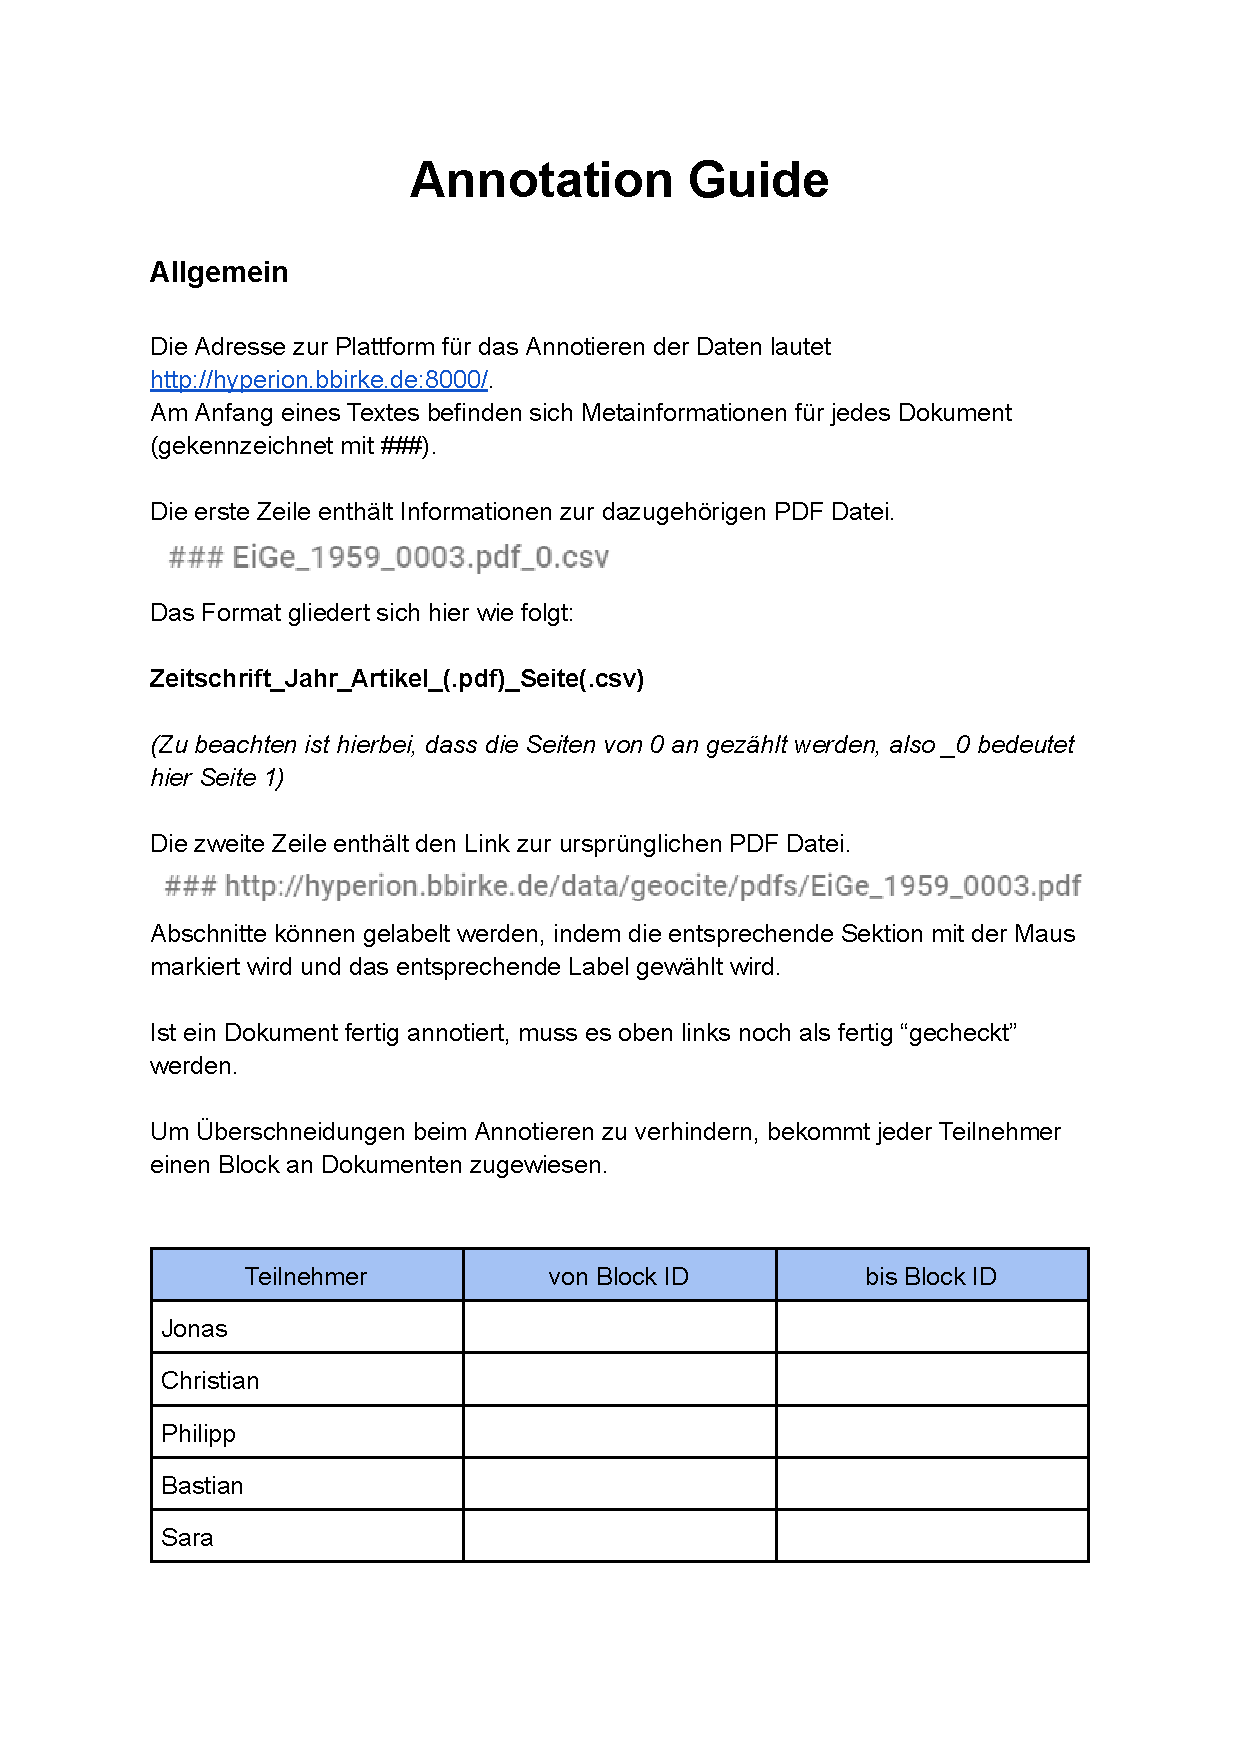
\includepdf[pages={1-}, scale=1]{includes/annotation_guide.pdf}
\end{appendices}
\newpage


%%%%%%%%%%%%%%%%%%%%%%%%%%%%%%%%%%%%%%%%%%%%%%%%%%%%%%%%%%%%%%%%%%%%%%%%%%%%%%%%%%%%%%%%%
\backmatter

% -- Bibliography
\printbibliography

%\printglossary[type=\acronymtype]

%\printglossary

\glsaddallunused[\acronymtype]

% -- Eidesstattliche Erklärung (= Affadavit)
% !TeX spellcheck = de_DE
% !TeX encoding = UTF-8

\chapter{Eidesstattliche Erkl\"arung}

	Hiermit versichere ich, dass ich diese \thesisType{} selbstst\"andig und ohne Benutzung anderer als der angegebenen Quellen und Hilfsmittel angefertigt habe und alle Ausf\"uhrungen, die w\"ortlich oder sinngem\"a\ss{} übernommen wurden, als solche gekennzeichnet sind, sowie, dass ich die \thesisType ~in gleicher oder \"ahnlicher Form noch keiner anderen Pr\"ufungsbeh\"orde vorgelegt habe.

	\vspace{3cm}

	Passau, \thedate

	\vspace{2cm}

	\parbox{8cm}{
		\hrule \strut \theauthor
	}




\end{document}